\documentclass[journal,compsoc]{IEEEtran}

\usepackage{cite}
%\usepackage{natbib}
\usepackage[font=footnotesize, labelfont=bf, skip=0pt]{caption}
\captionsetup{compatibility=false} % Prevents the warning
% Adjust the spacing
\captionsetup[figure]{skip=0pt}    % Adjust the value as needed
\captionsetup[table]{skip=0pt}    % Adjust the value as needed

\usepackage{comment}
\usepackage{amsmath,amssymb,amsfonts}
\usepackage{algorithm}
\usepackage{algpseudocode}
\usepackage{graphicx}
\usepackage{textcomp}
\usepackage[dvipsnames]{xcolor}
\usepackage[hidelinks]{hyperref}
\usepackage{pgfplots}
\pgfplotsset{compat=newest}
\usepackage{enumitem}
\DeclareMathOperator*{\argmax}{arg\,max}

\allowdisplaybreaks[3]


\usepackage{amsthm} % allows example and proof environment to be defined/used
\usepackage{mathtools}
\DeclarePairedDelimiter\ceil{\lceil}{\rceil}
\DeclarePairedDelimiter\floor{\lfloor}{\rfloor}
\newtheorem{example}{Example}[section]
\newtheorem{theorem}{Theorem}
\newtheorem{lemma}[theorem]{Lemma}
\newtheorem{problem}[theorem]{Problem}
\newtheorem{conj}[theorem]{Conjecture}
\newtheorem{defn}[theorem]{Definition}
\newtheorem{prop}[theorem]{Property}
\newtheorem{IP}[theorem]{Integer Linear Program}
\newtheorem{LP}[theorem]{Linear Program}
\newtheorem{proced}[theorem]{Procedure}
\newtheorem{algo}[theorem]{Algorithm}
\newtheorem{assum}[theorem]{Assumption}
\newtheorem{case}[theorem]{Case}
\newtheorem{remark}[theorem]{Remark}
%%% END Article customizations

%%% Document Parameters 
\setlength{\tabcolsep}{5pt}

\begin{document}


\title{Submodular Optimization with Predictions}
%
%
% author names and IEEE memberships
% note positions of commas and nonbreaking spaces ( ~ ) LaTeX will not break
% a structure at a ~ so this keeps an author's name from being broken across
% two lines.
% use \thanks{} to gain access to the first footnote area
% a separate \thanks must be used for each paragraph as LaTeX2e's \thanks
% was not built to handle multiple paragraphs
%
%
%\IEEEcompsocitemizethanks is a special \thanks that produces the bulleted
% lists the Computer Society journals use for "first footnote" author
% affiliations. Use \IEEEcompsocthanksitem which works much like \item
% for each affiliation group. When not in compsoc mode,
% \IEEEcompsocitemizethanks becomes like \thanks and
% \IEEEcompsocthanksitem becomes a line break with idention. This
% facilitates dual compilation, although admittedly the differences in the
% desired content of \author between the different types of papers makes a
% one-size-fits-all approach a daunting prospect. For instance, compsoc 
% journal papers have the author affiliations above the "Manuscript
% received ..."  text while in non-compsoc journals this is reversed. Sigh.

\author{Tianming~Zhao,~\IEEEmembership{Member,~IEEE,}
        Zhiyun~Jiang, 
        Chunqiu~Xia,
        Xinwei~Ji,
        Wei~Li,~\IEEEmembership{Senior Member,~IEEE,}
        and~Albert~Y.~Zomaya,~\IEEEmembership{Fellow,~IEEE}% <-this % stops a space
%\IEEEcompsocitemizethanks{\IEEEcompsocthanksitem M. Shell was with the Department
%of Electrical and Computer Engineering, Georgia Institute of Technology, Atlanta,
%GA, 30332.\protect\\
% note need leading \protect in front of \\ to get a newline within \thanks as
% \\ is fragile and will error, could use \hfil\break instead.
%E-mail: see http://www.michaelshell.org/contact.html
%\IEEEcompsocthanksitem J. Doe and J. Doe are with Anonymous University.}% <-this % stops an unwanted space
%\thanks{Manuscript received April 19, 2005; revised August 26, 2015.}

\thanks{T. Zhao, Z. Jiang, C. Xia, X. Ji, W. Li, and A. Y. Zomaya are with School of Computer Science, The University of Sydney, NSW 2006, Australia (e-mails: tzha2101@uni.sydney.edu.au, zjia5638@uni.sydney.edu.au, chunqiu.xia@sydney.edu.au, xiji3593@uni.sydney.edu.au, weiwilson.li@sydney.edu.au, and albert.zomaya@sydney.edu.au).}

}


% note the % following the last \IEEEmembership and also \thanks - 
% these prevent an unwanted space from occurring between the last author name
% and the end of the author line. i.e., if you had this:
% 
% \author{....lastname \thanks{...} \thanks{...} }
%                     ^------------^------------^----Do not want these spaces!
%
% a space would be appended to the last name and could cause every name on that
% line to be shifted left slightly. This is one of those "LaTeX things". For
% instance, "\textbf{A} \textbf{B}" will typeset as "A B" not "AB". To get
% "AB" then you have to do: "\textbf{A}\textbf{B}"
% \thanks is no different in this regard, so shield the last } of each \thanks
% that ends a line with a % and do not let a space in before the next \thanks.
% Spaces after \IEEEmembership other than the last one are OK (and needed) as
% you are supposed to have spaces between the names. For what it is worth,
% this is a minor point as most people would not even notice if the said evil
% space somehow managed to creep in.



% The paper headers
\markboth{IEEE Transactions on Pattern Analysis and Machine Intelligence}%
{}
% The only time the second header will appear is for the odd numbered pages
% after the title page when using the twoside option.
% 
% *** Note that you probably will NOT want to include the author's ***
% *** name in the headers of peer review papers.                   ***
% You can use \ifCLASSOPTIONpeerreview for conditional compilation here if
% you desire.



% The publisher's ID mark at the bottom of the page is less important with
% Computer Society journal papers as those publications place the marks
% outside of the main text columns and, therefore, unlike regular IEEE
% journals, the available text space is not reduced by their presence.
% If you want to put a publisher's ID mark on the page you can do it like
% this:
%\IEEEpubid{0000--0000/00\$00.00~\copyright~2015 IEEE}
% or like this to get the Computer Society new two part style.
%\IEEEpubid{\makebox[\columnwidth]{\hfill 0000--0000/00/\$00.00~\copyright~2015 IEEE}%
%\hspace{\columnsep}\makebox[\columnwidth]{Published by the IEEE Computer Society\hfill}}
% Remember, if you use this you must call \IEEEpubidadjcol in the second
% column for its text to clear the IEEEpubid mark (Computer Society jorunal
% papers don't need this extra clearance.)



% use for special paper notices
%\IEEEspecialpapernotice{(Invited Paper)}



% for Computer Society papers, we must declare the abstract and index terms
% PRIOR to the title within the \IEEEtitleabstractindextext IEEEtran
% command as these need to go into the title area created by \maketitle.
% As a general rule, do not put math, special symbols or citations
% in the abstract or keywords.
\IEEEtitleabstractindextext{%
\begin{abstract}
Submodular optimization is fundamental to artificial intelligence, underpinning tasks in data-driven decision-making and information summarization. In practice, however, the submodular objective often remains unknown or partially known due to limited data access or inherent complexities in its measurement. To address this, we consider the novel problem of maximizing an unknown submodular function under the cardinality constraint within a learning-augmented framework. We introduce a new and effective prediction error metric defined in the marginal gain space to address the limitations of existing metrics that operate in the raw function space. We show that the R-step predictive greedy algorithm achieves an approximation ratio $1 - (1 - \frac{1}{\eta {\lceil \frac{K}{R} \rceil}})^{\lceil \frac{K}{R} \rceil}$, where $K$ is the cardinality constraint and $\eta$ is the proposed error metric. This ratio is bounded by $1 - e^{-1/\eta}$, ensuring optimal consistency. The effectiveness of our approach is evaluated across three applications: machine learning feature selection, influence maximization, and text summarization, using real-world datasets. Experimental results highlight the robustness of the R-step predictive greedy algorithm to prediction quality, maintaining near-optimal performance even with significant errors. 
\end{abstract}

% Note that keywords are not normally used for peerreview papers.
\begin{IEEEkeywords}
Learning-augmented algorithms, submodular functions, optimization, predictions
\end{IEEEkeywords}
}


% make the title area
\maketitle
\IEEEdisplaynontitleabstractindextext
% \IEEEdisplaynontitleabstractindextext has no effect when using
% compsoc or transmag under a non-conference mode.

\IEEEpeerreviewmaketitle


\section{Introduction}

Submodular optimization has pervasive applications in machine learning and pattern recognition. The diminishing returns property of submodular functions naturally captures the redundancy and diversity trade-offs common in real-world optimization scenarios, such as image summarization~\cite{submodularOptNoisetoImageCollection}, influence maximization~\cite{mossel2010submodularity}, and feature selection~\cite{feature-selection}. Advancing algorithmic solutions for submodular optimization can significantly impact a broad range of problems~\cite{Krause_Golovin_2014}. 

A critical yet frequently overlooked issue in practical submodular optimization is the inaccessibility or inherent uncertainty of the target submodular function. Unlike theoretical settings where the objective function is assumed to be known and directly queryable, real-world applications involve scenarios where the function cannot be directly evaluated. The causes include unseen out-of-sample data, expensive query of the function, and no universally agreed functional form of the objective. Hence, the design and analysis of algorithms capable of handling submodular optimization for uncertain or unknown functions are needed. 

In this work, we address this practical challenge by introducing a learning-augmented framework where predictions, rather than the exact values, of the submodular function guide the optimization process. The study of submodular optimization for uncertain functions is not new. See, for example,~\cite{submodularOptNoisetoImageCollection,submodularOptNoise,horel2016maximization}. However, our work departs from previous pessimistic findings by proposing an intuitive, effective error metric defined in the marginal gain space. This novel metric enables theoretical guarantees of simple algorithms that smoothly degrade with prediction errors, leading to a practical and effective optimization validated through extensive experiments. 


%The study of submodular optimization is an interesting subject from both a theoretical and a practical point of view. Applications in artificial intelligence include active learning \cite{golovin2011adaptive}, text summarization \cite{lin2011class}, and information diffusion in networks \cite{kempe2003maximizing}. 

To formalize our problem, we consider the task of maximizing an \textit{unknown} submodular function within a learning-augmented framework. A real-valued function $f: 2^N \rightarrow \mathbb{R}$ defined over subsets of a finite ground set $N$ is submodular if it satisfies the following inequality for all $S, T \subseteq N$:
\[ f(S) + f(T) \geq f(S \cup T) + f(S \cap T) \]

It is equivalent to defining submodularity via a diminishing gains property. Let $d_B(A) = f(A \cup B) - f(A)$ denote the \textit{marginal gain} of set $B$ to $A$, for any $A, B \subseteq N$. Then, function $f$ is submodular if for all $A \subseteq B \subseteq N, C \subseteq N \backslash B$: 
\[ d_{C}(A) \geq d_{C}(B) \]

We consider the problem of maximizing a submodular function $f$ under a \textit{cardinality constraint}: 
\begin{equation} \label{problem}
\max_{S \subseteq N}\{ f(S): |S| \leq K, f ~\text{submodular} \}
\end{equation}

For simplicity, we assume a \textit{normalized} submodular function, i.e., $f(\emptyset) = 0$. 
A classic assumption is that $f$ is accessible via a \textit{value oracle}, which may require a representation exponential in $|N|$. However, $f$ is often inaccessible due to (1) lack of data or (2) an unknown functional form. Consider the ML feature selection task that aims to find a set of features from some feature space $N$ to train a model to optimize out-of-sample performance $f$. Out-of-sample performance $f$ cannot be measured as the data are unknown. Consider the text summarization task that aims to find a set of tokens from the text $N$ to maximize the summarization quality. Summarization quality cannot be measured as the functional form to measure the quality is unknown. Therefore, we assume that the function $f$ is \textit{unknown} to the algorithm. However, a \textit{predictor} $\tilde{f}$ for $f$ is visible, which returns $\tilde{f}(S)$ for any set $S$ but may introduce errors. Specifically, we are not allowed to query the target submodular function $f$ to get values $f(S)$ for any set $S$. Instead, we could query a learned oracle that gives us predicted values $\tilde{f}(S)$ for $f(S)$. 
This setting overcomes the issue with the exponential representation of $f$, as the Machine Learning (ML) model can learn functions with compact representation, often with just $O(\text{poly}(N))$ space. Recent works have further shown the learnability of submodular functions \cite{approxSubmodularFunctions,learnValueFunctions,representationApproxLearnSubmodularFunctions,submodularFunctionsLearn}, which supports the practicality of our framework.



Submodular optimization under an unknown submodular function has been studied by~\cite{submodularOptNoisetoImageCollection,submodularOptNoise,horel2016maximization}. The predictor $\tilde{f}$ may be imperfect and comes with errors. The existing work defines the prediction error as $\max_{S \subseteq N}{\frac{|\tilde{f}(S) - f(S)|}{f(S)}}$, which penalizes the absolute percentage gap between predictions and exact values \cite{submodularOptNoise}. A pessimistic result has been shown: the celebrated greedy algorithm \cite{greedySubmodularFunctions} fails to obtain an approximation strictly better than $O(\frac{1}{K})$ for any constant error, and no algorithm is robust to a small error. We argue that this pessimism is because the error metric penalizes the predictions in the raw submodular function space rather than the marginal gain space. Take the greedy algorithm as an example. The algorithm starts with an empty set and iteratively adds the element from $N$ with the maximum positive marginal gain until the set reaches size $K$. Decisions are purely based on marginal gains, not the raw function values. This motivates an alternative, perhaps a more proper error metric that penalizes the errors in the marginal gain space. It is natural to consider the following question:
\begin{center}
\textit{What is a proper error metric for predictions in submodular optimization, and what is the performance of the greedy algorithm under this error metric in theory and practice?}
\end{center}


\subsection{Performance metrics}

% Define approximation ratio
%We analyze the performance of an algorithm by its approximation ratio. 
An \textit{$\alpha$-approximation algorithm} $A$ for a maximization problem is an algorithm with $\text{OPT}(I) \leq \alpha \cdot A (I)$, for any problem instance $I$, where $\text{OPT}(I)$ and $A(I)$ are the optimal value and the value obtained by algorithm $A$ on $I$. The ratio $\alpha$, which is allowed to be a function in the problem input and the prediction error, is called the approximation ratio. %\textcolor{purple}{We obtained the predicted optimal submodular values demonstrated visually instead of the sole optimal values in the experimental part. Indeed, the predicted values, satisfying the proposed approximation ratio, are compared with empirical baselines.}

% Consistency, Smoothness, Robustness
The literature on algorithms with predictions analyzes performance by \textit{consistency}, \textit{smoothness}, and \textit{robustness}. Consistency is defined to be the approximation ratio under perfect predictions, smoothness under any prediction, and robustness under worst-case predictions with large errors. If the error is $\eta$, an algorithm is said to have consistency $\tau$ (or be $\tau$-consistent) if it is $\tau$-approximation when the predictions coincide the exact values, have smoothness $\rho$ ($\rho$-smooth) if it is $\rho$-approximation where $\rho$ is a function in $\eta$, and have robustness $\upsilon$ ($\upsilon$-robust) if it is $\upsilon$-approximation under any $\eta$ where $\upsilon$ is independent of $\eta$. 


\subsection{Related work}

% Submodular Optimization dimension
\noindent \textbf{Submodular optimization.} Maximizing submodular functions has been extensively studied. The work \cite{greedySubmodularFunctions} shows the greedy heuristic is a $(1 - e^{-1})$-approximation for monotone submodular functions under the cardinality constraint and $\frac{1}{2}$ under the matroid constraint. No polynomial-time algorithm can obtain an approximation ratio better than $1 - e^{-1}$ under the cardinality constraint unless $\text{P}=\text{NP}$, representing a theoretical upper bound \cite{setCoverisHard}. For non-monotone submodular optimization, \cite{maximizingNonMonotoneSubmodularFunctions} gives a deterministic local search $\frac{1}{3}$-approximation and a randomized $\frac{2}{5}$-approximation for non-negative functions. For unconstrained maximization, \cite{linearTimeApproximationForUnconstrainedSubmodular} gives a randomized linear time $\frac{1}{2}$-approximation. 


% Learning Submodular Functions dimension
\noindent \textbf{Learning submodular functions.} Learnability is crucial for optimization with predictions. Prior works have shown that submodular functions are learnable from a few observations. %, enabling optimization with predictions for the applications where accessing the function is costly or impossible. 
There exists an algorithm that requires $\text{poly}(|N|)$ oracle queries to output a submodular function $\tilde{f}$ approximating the exact function within a factor $O(\sqrt{|N|}\log |N|)$ for monotone submodular functions \cite{approxSubmodularFunctions}. 
%\cite{approxSubmodularFunctions} gives a deterministic algorithm that makes $\text{poly}(|N|)$ oracle queries and derives a submodular function $\tilde{f}$ approximating the ground truth function within a factor $O(\sqrt{|N|}\log |N|)$ for general monotone submodular functions. 
The work \cite{representationApproxLearnSubmodularFunctions} shows that a low-rank decision tree can approximate every submodular function, enabling an efficient learning scheme. 
Furthermore, the work \cite{submodularFunctionsLearn} considers the learnability of submodular functions in a distributional PAC-style setting. 


% Learning-augmented Algorithms dimension
\noindent \textbf{Optimization with predictions.} Recent works have shown the potential of using predictions to improve optimization with proven guarantees. Applications span the fields of scheduling, caching, secretary, matching, and graphs \cite{ImproveOnlineAlgorithmsViaML,cachingWithPredictions,secretaryWithPredictions,matchingWithPredictions,errorMetricsForGraphs}. To our knowledge, no prior work on submodular optimization with predictions under errors designed for the worst-case performance analysis exists. A relevant work is by \cite{learningAugmentedSubmodularUpdates} on dynamic submodular maximization, where predictions are used to reduce the dynamic update time. %In contrast to their focus on predictions aiding in pre-processing, our work is on using predictions for approximation ratio.

Prior works on submodular optimization under noise assume the queries to the submodular function have small additive errors independently drawn from an identical distribution (i.i.d). Then, efficient algorithms exist with an approximation ratio arbitrarily close to $1 - e^{-1}$ \cite{submodularOptNoise}. 
Other related works include maximizing approximately submodular functions \cite{maximizingApproximatelySubmodularFunctions}, minimizing submodular functions under noise \cite{minimizingSubmodularFunctionsUnderNoise}, and the application to image summarization \cite{submodularOptNoisetoImageCollection}.

\subsection{Our results}

\noindent \textbf{Prediction error metric in the marginal gain space.} 
We propose a simple prediction error metric $\eta$ in the marginal gain space. It penalizes the multiplicative gap between the marginal gain prediction and the true value, i.e., $\tilde{f}(A \cup B) - \tilde{f}(A)$ versus ${f}(A \cup B) - {f}(A)$, for $A, B \subseteq N$. We discuss the key differences between this metric and the existing one. %Subsequently, we show that with this error metric, the celebrated greedy algorithms achieve an optimal consistency and a smoothness as a function of $\eta$. 
%We show that with this error metric, the celebrated greedy algorithms achieve optimal consistency and smoothness as a function of $\eta$. 

\noindent \textbf{Performance analysis for the greedy algorithms.}
We analyze the performance of the single-step and $R$-step predictive greedy algorithms. The former is a straightforward application of the greedy algorithm \cite{greedySubmodularFunctions}; the latter is an extension of it. The results we obtain include: (1) the single-step predictive greedy achieves, for any non-decreasing $f$, an approximation ratio of $1 - (1 - \frac{1}{\eta K})^K$, bounded by $1 - e^{-1/{\eta}}$ degrading smoothly with $\eta$, (2) the $R$-step predictive greedy achieves, for any non-decreasing $f$, an approximation ratio of $1 - (1 - \frac{1}{\eta {\lceil \frac{K}{R} \rceil}})^{\lceil \frac{K}{R} \rceil}$, also bounded by $1 - e^{-1/{\eta}}$, and (3) the algorithm achieves an approximation ratio of $\frac{1}{\lambda} \cdot (1 - (1 - \frac{1}{K})^K)$ if the predictor $\tilde{f}$ is submodular and non-decreasing, where $\lambda$ is the prediction error defined in the raw function space. 
%The results apply to general submodular function $f$.%, not limited to non-decreasing ones. 
%The results are more general than those mentioned above, which 


\noindent \textbf{Experimental evaluations for the greedy algorithms.}
We consider three applications of submodular optimization with predictions: ML feature selection, influence maximization, and text summarization. We evaluate the greedy algorithms on these applications with real-world data and compare them against the existing baselines. The predictive greedy is robust to prediction errors, observing a near-optimal performance on many tasks even under large errors. 


 

\subsection{Technical contributions}

The prediction error metric $\eta$ proposed by this paper is new in submodular optimization, which accounts for predictions that are under or over-estimating the exact values. It applies to non-monotone, non-positive functions. Defining the error as the product of under- and over-estimation factors follows the spirit of \cite{FlowTimeScheduling} with the same construct for the prediction error in scheduling with predictions.

The algorithm considered in this paper is an extension of work by \cite{greedySubmodularFunctions}. The previous analysis results are for monotone functions. We give a simple and direct proof for any function and establish a unified bound for the single-step and R-step greedy. Setting $R = 1$ or restricting to monotone functions, our results match the existing bounds, showing the tightness of the analysis. If the predictor is submodular, we show that the bounds can be derived as a function in the error metric defined in the raw function space. This will leverage works of \cite{approxSubmodularFunctions} that produce submodular predictors. 

The submodular optimization framework with predictions is practical, as demonstrated through three applications: ML feature selection, influence maximization, and text summarization. We observe that the predictive greedy algorithm performs well on many tasks, even if the prediction errors are unreasonably large. These promising results show the framework's practicality and demonstrate its reliability in complex real-world tasks.



\section{Prediction error metric} \label{sec:prediction error metric}

Let $\tilde{d}_B(A) = \tilde{f}(A \cup B) - \tilde{f}(A)$ denote the marginal gain prediction. Define:
\[\eta_u = \max_{A,B \subseteq N}{\frac{d_B(A)}{\tilde{d}_B(A)}}, \eta_o = \max_{A,B \subseteq N}{\frac{\tilde{d}_B(A)}{d_B(A)}}\] 
as the maximum underestimation/overestimation factors. Therefore, for any two sets $A, B \subseteq N$, we have:
\[ \frac{d_B(A)}{\eta_u} \leq \tilde{d}_B(A) \leq \eta_o \cdot d_B(A), ~\forall A, B \subseteq N \]
Define the total prediction error $\eta = \eta_u \cdot \eta_o$. 
With the complete set of predictions and exact values, one may compute the prediction error $\eta$ of the predictor $\tilde{f}$ with respect to a problem instance. Ideally, the algorithm does not require $\eta$ a priori (a property our algorithm achieves); we desire the algorithm's performance tied to $\eta$. Note that the error measurement uses the maximum multiplicative gap to capture the notion of distance, but this is not binding. As long as the error is in the marginal gain space, other forms like $L_1$ distance also work, which may result in the approximation ratio having a different dependency on the error. In line with the error metrics defined for other recent leaning-augmented algorithms \cite{SchedulingViaWeights, FlowTimeScheduling, RealTimeSchedulingwithPredictions}, we focus on the maximum multiplicative gap in this work.


We first show that, for any deterministic algorithm to achieve an approximation ratio, the prediction error must be \textit{finite}, meaning that the marginal gain prediction is zero if and only if the actual gain is zero, and \textit{directionally consistent}, meaning that the marginal gain prediction and the actual gain have the same sign. 
\begin{lemma} [Necessity of finite and directionally consistent error] \label{lem:necessity-of-error-properties}
A deterministic $c$-approximation ($c > 0$) algorithm exists for problem (\ref{problem}), only if (1) the prediction error is finite, i.e., $\tilde{d}_B(A) = 0 \iff {d}_B(A) = 0, \forall A, B \subseteq N$ and (2) the error is directional consistent, i.e., $\tilde{d}_B(A) \cdot {d}_B(A) \geq 0, \forall A, B \subseteq N$.
\end{lemma} 
\begin{proof}
We first show that the error must be finite. Construct two simple instances of problem (\ref{problem}) denoted by $I_1$ and $I_2$ as follows. Both instances have $N = \{ a, b \}$ and $K = 1$. Instance $I_1$ has $f(\{a\}) = 1, f(\{b\}) = 0$; instance $I_2$ has $f(\{ a \}) = 0$, $f(\{ b \}) = 1$. The optimal value for both instances is $1$. Suppose the algorithm can access a predictor $\tilde{f}$ with $\tilde{f}(\emptyset) = 0, \tilde{f}(\{a\}) = 1, \tilde{f}(\{b\}) = 1$. Any deterministic algorithm returns either set $\{ a \}$ or $\{ b \}$ or $\emptyset$, which produces a value of $0$ for $I_2$ if returning set $\{ a \}$ or $0$ for $I_1$ if returning set $\{ b \}$ or $0$ for both. This is, at best, a $0$-approximate algorithm. The argument also holds with $\tilde{f}(\emptyset) = \tilde{f}(\{a\}) = \tilde{f}(\{b\}) = 0$. Therefore, we must have $\tilde{d}_B(A) = 0 \iff {d}_B(A) = 0, \forall A, B \subseteq N$ to have $c$-approximation ($c > 0$). 

We then show that the error must be directionally consistent using a similar construction. This time, instance $I_1$ has $f(\{a\}) = 1, f(\{b\}) = -1$; instance $I_2$ has $f(\{ a \}) = -1$, $f(\{ b \}) = 1$. The optimal value for both instances is still $1$. Suppose that $\tilde{f}(\emptyset) = 0, \tilde{f}(\{a\}) = 1, \tilde{f}(\{b\}) = 1$. Any deterministic algorithm returns either set $\{ a \}$ or $\{ b \}$ or $\emptyset$, which produces a value of $-1$ for $I_2$ if returning set $\{ a \}$ or $-1$ for $I_1$ if returning set $\{ b \}$ or $0$ for both. Again, this is, at best, $0$-approximation. 
\end{proof}


%\subsection*{Difference with the previous error metrics}
Lemma \ref{lem:necessity-of-error-properties} indicates that no algorithm is robust to prediction errors, i.e., no $c$-approximation algorithm exists with $c$ independent of $\eta$. This is intuitive, as the worst predictions provide no information for $f(S), \forall S \subseteq N$, so any algorithm can do no better than randomly selecting a subset. 

The proposed error metric $\eta$ is new and fundamentally different from the existing one: $\epsilon \coloneqq \max_{S \subseteq N}{\frac{|\tilde{f}(S) - f(S)|}{f(S)}}$, or predictor $\tilde{f}$ is $\epsilon$-erroneous if $(1 - \epsilon) f(S) \leq \tilde{f}(S) \leq (1 + \epsilon) f(S), \forall S \subseteq N$ \cite{submodularOptNoise}. Note that $\epsilon$-error is defined for non-negative functions, but $\eta$-error has no such limit. For any non-negative function $f$, the $\eta$-error is more restrictive than $\epsilon$-error: any $\epsilon$-erroneous predictor, even with an arbitrarily small $0 < \epsilon < 1$, may have an infinite $\eta$-error, while any predictor with an $\eta$-error has an $\epsilon$-error bounded by $\max \{ 1 - \frac{1}{\eta_u}, \eta_o - 1 \}$.

\begin{lemma} \label{lem:any-epsilon-error-can-be-infite-eta}
For any fixed $0 < \epsilon < 1$, there exists a $\epsilon$-erroneous predictor $\tilde{f}$ with an infinite $\eta$. 
\end{lemma}
\begin{proof}
Let $N = \{a, b\}, f(\emptyset) = 0, f(\{a\}) = 1, f(\{ b \}) = \frac{2\epsilon}{1 - \epsilon}, f(\{ a, b \}) = \frac{1 + \epsilon}{1 - \epsilon}, \tilde{f}(\emptyset) = 0, \tilde{f}(\{ a \}) = 1 + \epsilon, \tilde{f}(\{ b \}) = \frac{2 \epsilon}{1 - \epsilon}, \tilde{f}(\{ a, b \}) = 1 + \epsilon$. This yields a $\epsilon$-erroneous predictor $\tilde{f}$ with an infinite $\eta$, as $d_{\{ b \}}(\{ a \}) = \frac{2 \epsilon}{1 - \epsilon}$ and $\tilde{d}_{\{ b \}}(\{ a \}) = 0$. 
\end{proof}

\begin{lemma} \label{lem:any-eta-error-has-bounded-epsilon-error}
Any predictor $\tilde{f}$ for a non-negative function $f$ with error $\eta = \eta_u \cdot \eta_o$ is $\epsilon$-erroneous with $\epsilon \leq \max \{ 1 - \frac{1}{\eta_u}, \eta_o - 1 \}$. 
\end{lemma}
\begin{proof}
For any $S \subseteq N$, we have $\frac{d_{\emptyset}(S)}{\eta_u} \leq \tilde{d}_{\emptyset}(S) \leq \eta_o \cdot d_{\emptyset}(S) \Rightarrow \frac{f(S)}{\eta_u} \leq \tilde{f}(S) \leq \eta_o \cdot f(S) \Rightarrow \frac{1}{\eta_u} - 1 \leq \frac{\tilde{f}(S) - f(S)}{f(S)} \leq \eta_o - 1 \Rightarrow \frac{|\tilde{f}(S) - f(S)|}{f(S)} \leq \max \{ 1 - \frac{1}{\eta_u}, \eta_o - 1 \}$.  
\end{proof}

In the following section, we will assume that the prediction errors are finite and directionally consistent. Under such conditions, we show that algorithms with quality scaled smoothly with prediction errors exist. 



\section{Optimization with predictions} \label{sec:optimization-with-predictions}


A natural extension of the classic greedy algorithms is to start from an empty set and iteratively add elements: at each step, the chosen set of elements $I$ (which could have more than one element) maximize $\tilde{d}_{I}(S)$ constrained by the size of $I$, where $S$ is the set obtained in the previous step. We name this procedure \textit{R-step predictive greedy heuristic}, if we constrain $|I| \leq R$. If $R$ is set to one, the algorithm simplifies to \textit{single-step predictive greedy}. We will first analyze the performance of the single-step greedy and then generalize the analysis to the $R$-step greedy. 

\subsection{The single-step predictive greedy heuristic}

\begin{algorithm} [tb]
\caption{Single-step Predictive Greedy} \label{algo:single-step-greedy}
\begin{algorithmic}[1]
\State \textbf{Input:} finite set $N$, marginal gain predictions $\tilde{d}$, and the cardinality constraint $K$
\State \textbf{Output:} set $S$ with $|S| \leq K$
\State initialize $S^0 \gets \emptyset$, $t \gets 0$

\While{$|S^{t}| < K$}
    \State $e_t \gets \argmax_{e \in {N - S^t}}{\tilde{d}_{\{e\}}(S^{t})}$
    %\State let $e_t \in N - S^t$ such that $\tilde{d}_{\{e_t\}}(S^{t}) = \max_{e \in {N - S^t}}{\tilde{d}_{\{e\}}(S^{t})}$, with ties break arbitrarily
    \State $\tilde{d}_{t} \gets \tilde{d}_{\{e_t\}}(S^{t})$%, ${d}_{t} \gets {d}_{\{e_t\}}(S^{t})$
    \If{$\tilde{d}_{t} > 0$}
        \State $S^{t+1} \gets S^{t} \cup \{ e_t \}$, $t \gets t + 1$ \Comment{add $e_t$ to set $S^{t}$}
    \Else 
        \State \textbf{break} \Comment{stop with set $S^{t}$}
    \EndIf 
\EndWhile
\State $K^* \gets |S^{t}|$ \Comment{$K^*$ is the size of the output set}
\State \textbf{return} \( S^{t} \)
\end{algorithmic}
\end{algorithm}

The single-step greedy, at iteration $t$, chooses one element $e_t$ that maximizes $\tilde{d}_{\{e_t\}}(S^{t})$, where $S^t$ is the set obtained in the previous step. Algorithm \ref{algo:single-step-greedy} gives the pseudo-code. Let $F^{\textsf{OPT}}$ be the value of an optimal solution to problem (\ref{problem}) and $F^{\textsf{PG}}$ the value of a particular solution constructed by Algorithm \ref{algo:single-step-greedy}. We assume $K^* \geq 1$ to exclude trivial problems where $F^{\textsf{OPT}} = 0$ and $\tilde{d}_{0} \leq 0 \Rightarrow d_{\{e\}}(\emptyset) \leq 0, \forall e \in N$ and $F^{\textsf{PG}} = f(\emptyset) = 0$ due to directional consistency of the errors. We begin with the following property for general submodular set functions.

\begin{lemma} [\cite{greedySubmodularFunctions}] \label{lem:bound-property}
If $f$ is a submodular set function on $N$ with $\theta(f) = - \min_{S \subseteq N, e \in N - S}{d_{\{e\}}{(S)}}$, then:
\[ f(T) \leq f(S) + \sum_{e \in T - S}{d_{\{e\}}(S)} + |S-T| \theta(f), ~~~ \forall S, T \subseteq N \]
\end{lemma}

We introduce the $\theta$ function, where $-\theta(f)$ denotes the minimum value of any single element's marginal gain, i.e.,  
$\theta(f) = - \min_{S \subseteq N, e \in N - S}{d_{\{e\}}{(S)}}$.
The function $f$ is non-decreasing if and only if $\theta(f) \leq 0$. The bound on $F^{\textsf{PG}}$ is a function in the value $\theta(f)$. In the following analysis, we use $d_t$ to denote the actual marginal gain of adding $e_t$ at the $t$-th iteration, i.e., $d_t = {d}_{\{e_t\}}(S^{t})$. 


\begin{lemma} \label{lem:bounds on f(S^t)}
$F^{\textsf{OPT}} \leq f(S^t) + K \cdot \eta \cdot d_{t} + t \cdot \max \{ 0, \theta(f) \}, ~~~ t = 0, ..., K^*-1 ~(\textit{including } K^* \textit{ if } K^* < K)$.
\end{lemma}
\begin{proof}
Fix any $t = 0, ..., K^* - 1 ~(\textit{including } K^* \textit{ if } K^* < K)$. 
For any $e \in N - S^t$, we have $\tilde{d}_{\{e\}}(S^{t}) \leq \tilde{d}_{\{e_t\}}(S^{t})$, by the selection of $e_t$. Therefore, it holds that:
\[ d_{\{e\}}(S^t) \leq \eta_u \cdot \tilde{d}_{\{e\}}(S^{t}) \leq \eta_u \cdot \tilde{d}_{\{e_t\}}(S^{t}) \leq \eta_u \cdot \eta_o \cdot {d}_{\{e_t\}}(S^{t}) \]
which means $d_{\{e\}}(S^t) \leq \eta \cdot d_t$. 
Let $T$ be the optimal set to problem (\ref{problem}). We have $\tilde{d}_t > 0 \Rightarrow d_t > 0$ and $\sum_{e \in T - S^t}{d_{\{e\}}(S^t)} \leq \sum_{e \in T - S^t}{\eta \cdot d_t} \leq |T - S^t| \cdot \eta \cdot d_t \leq K \cdot \eta \cdot d_t$.
We have $|S^t-T| \theta(f) \leq |S^t-T| \cdot \max \{ 0, \theta(f) \} \leq t \cdot \max \{ 0, \theta(f) \}$. 
By Lemma \ref{lem:bound-property}, we have:
\begin{align*}
    F^{\textsf{OPT}} &\leq f(S^t) + \sum_{e \in T - S^t}{d_{\{e\}}(S^t)} + |S^t-T| \theta(f) \\
    &\leq f(S^t) + K \cdot \eta \cdot d_{t} + t \cdot \max \{ 0, \theta(f) \} \qedhere
\end{align*}
\end{proof}

\begin{theorem} [Bounds on Single-step Predictive Greedy] \label{thm:bounds-on-SPG}
If the single-step predictive greedy is applied and stops after $K^* \leq K$ steps, we have:
\begin{align*}
& \frac{F^{\textsf{PG}} + K^* \cdot \max \{ 0, \theta(f) \}}{F^{\textsf{OPT}}} \geq 1,           & K^* < K\\
& \frac{F^{\textsf{PG}} + K \cdot \max \{ 0, \theta(f) \}}{F^{\textsf{OPT}}} \geq 1 - (1 - \frac{1}{\eta K})^K,  & K^* = K
\end{align*}
\end{theorem}
\begin{proof}
\textbf{Case 1 ($K^* < K$).} Let $T$ be the optimal set to problem (\ref{problem}). We have $\tilde{d}_{K^*} \leq 0 \Rightarrow {d}_{K^*} \leq 0$. By Lemma \ref{lem:bounds on f(S^t)}, $F^{\textsf{OPT}} \leq f(S^{K^*}) + K \cdot \eta \cdot d_{K^*} + K^* \cdot \max \{ 0, \theta(f) \} \leq F^{\textsf{PG}} + K^* \cdot \max \{ 0, \theta(f) \}$.

\textbf{Case 2 ($K^* = K$).} Let $\alpha = 1 - \frac{1}{\eta K}$. By Lemma \ref{lem:bounds on f(S^t)}:
\[ F^{\textsf{OPT}} \leq f(S^t) + K \cdot \eta \cdot d_{t} + t \cdot \max \{ 0, \theta(f) \}, ~~~ t = 0, ..., K-1 \]
Substituting $\alpha = 1 - \frac{1}{\eta K}$ and $d_t = f(S^{t+1}) - f(S^t)$, multiplying by $\alpha^{K-t-1}$ for the $t$-th inequality, and re-arranging gives:
\begin{align*}
\alpha^{K-t-1} f(S^{t+1}) &\geq - {\max \{ 0, \theta(f) \}} \cdot (1 - \alpha) \cdot \alpha^{K-t-1} \cdot t  \\ &~~~~~~ + \alpha^{K-t} f(S^t) + {F^{\textsf{OPT}}} \cdot (1 - \alpha) \alpha^{K-t-1}
\end{align*}
for $t = 0, ..., K-1$. Summing all the inequalities (with $f(S^0) = f(\emptyset) = 0$), we have:
\begin{align*}
    &F^{\textsf{PG}} = f(S^K) \\
    \geq& - {\max \{ 0, \theta(f) \}} \cdot (1 - \alpha) \cdot \sum_{t=0}^{K-1}{\alpha^{K-t-1} \cdot t}  \\ 
    &~~~~~~+ {F^{\textsf{OPT}}} \cdot (1 - \alpha) \cdot \sum_{t=0}^{K-1}{\alpha^{K-t-1}} \\
    =& - {\max \{ 0, \theta(f) \}} \cdot (-\sum_{t=0}^{K-1}{\alpha^t} + K) + F^{\textsf{OPT}} \cdot (1 - \alpha^K) \\
    \geq& - {\max \{ 0, \theta(f) \}} \cdot K + F^{\textsf{OPT}} \cdot (1 - \alpha^K) \qedhere
\end{align*}
\end{proof}


Theorem \ref{thm:bounds-on-SPG} implies that, for any non-decreasing $f$, $F^{\textsf{PG}} = F^{\textsf{OPT}}$, meaning the single-step predictive greedy gives an optimal solution when the output has cardinality less than $K$. 
If the predictions are perfect, i.e., $\eta = 1$, the approximation ratio matches that of the single-step greedy heuristic with perfect information \cite{greedySubmodularFunctions}. Therefore, the single-step predictive greedy achieves optimal consistency. Observe that $1 - (1 - \frac{1}{\eta K})^K > 1 - \lim_{K \rightarrow \infty}{(1 - \frac{1}{\eta K})^K} \geq 1 - e^{-1/\eta}$. Therefore, Theorem \ref{thm:bounds-on-SPG} shows that, for any non-decreasing $f$: 
\[ \frac{F^{\textsf{PG}}}{F^{\textsf{OPT}}} \geq 1 - (1 - \frac{1}{\eta K})^K > 1 - e^{-1/\eta} \]
The analysis hold if we re-define the prediction error to be the maximum multiplicative gap between any single-element's marginal gain and its prediction, i.e., Theorem \ref{thm:bounds-on-SPG} holds if we let $\eta_u = \max_{A \subseteq N, e \in N}{\frac{d_{\{e\}}(A)}{\tilde{d}_{\{e\}}(A)}}, \eta_o = \max_{A \subseteq N, e \in N}{\frac{\tilde{d}_{\{ e \}}(A)}{d_{\{e\}}(A)}}$, and $\eta = \eta_u \cdot \eta_o$.

\subsection{The R-step predictive greedy heuristic}

\begin{algorithm}[tb]
\caption{R-step Predictive Greedy}
\label{alg:R-step-greedy}
\textbf{Input:} finite set \( N \), marginal gain predictions \( \tilde{d} \), step \( R \), and the cardinality constraint \( K \)\\
\textbf{Output:} set \( S \) with \( |S| \leq K \)
\begin{algorithmic}[1]  %[1] enables line numbers
\State Initialize \( S^0 \gets \emptyset \), \( t \gets 0 \), \( q \gets \lceil \frac{K}{R} \rceil \), \( r \gets qR - K \)
\While{\( |S^t| < K \)}
    \State $I^t \gets \argmax_{I \subseteq N - S^t, |I| \leq \min \{ R, K - |S^t| \}} {\tilde{d}_{I}(S^{t})}$
    %\State let $I^t \subseteq N - S^t$ s.t. $\tilde{d}_{I^t}(S^{t}) = \max_{I \subseteq N - S^t, |I| \leq \min \{ R, K - |S^t| \}}{\tilde{d}_{I}(S^{t})}$, ties break arbitrarily
    \State \( \tilde{d}_t \gets \tilde{d}_{I^t}(S^t) \) %, \( d_t \gets d_{I^t}(S^t) \)
    \If{\( \tilde{d}_t > 0 \)}
        \State \( S^{t+1} \gets S^t \cup I^t \), \( t \gets t + 1 \) \Comment{add \( I^t \) to set \( S^t \)}
    \Else
        \State \textbf{break} \Comment{stop with set \( S^t \)}
    \EndIf
\EndWhile
\State \( K^* \gets |S^t| \) \Comment{\( K^* \) is the size of the output set}
\State \textbf{return} \( S^t \)
\end{algorithmic}
\end{algorithm}

Suppose $K = q R - r$, where $q$ is a positive integer and $0 \leq r < R$. Then, at iteration $t$, the R-step greedy chooses at most $R$ elements (without violating the cardinality constraint) $I^t$ that maximize $\tilde{d}_{I^t}(S^t)$ constrained by $|I^t| \leq R$, where $S^t$ is the set obtained in the previous step. Algorithm \ref{alg:R-step-greedy} gives the pseudo-code. 
Let $F^{\textsf{RPG}}$ be the value of a particular solution constructed by the R-step predictive greedy. 


\begin{lemma} \label{lem:general-bound-property}
For any $S, T \subseteq N$, if $\{ J_1, ..., J_p \}$ is a partition of $T - S$, we have 
%If $f$ is a submodular set function on $N$ with $\theta(f) = - \min_{S \subseteq N, e \in N - S}{d_{\{e\}}{(S)}}$ and $\{ J_1, ..., J_p \}$ is a partition of $T - S$, then
$f(T) \leq f(S) + \sum_{i = 1}^{p}{d_{J_i}(S)} + |S-T| \theta(f)$.
\end{lemma}
\begin{proof}
Let $J_0 = \emptyset$ for the convention. We have:
\begin{align*}
&f(T) - f(S) \leq f(T \cup S) + |S-T| \theta(f) - f(S) \quad \textit{(\cite{greedySubmodularFunctions})} \\
&= \sum_{i=1}^{p}{f(S \cup \bigcup_{j=0}^{i}{J_j}) - f(S \cup \bigcup_{j=0}^{i-1}{J_j})} + |S-T| \theta(f) \\
%&=\sum_{i=1}^{p}{d_{J_i}{(S \cup \bigcup_{j=0}^{i-1}{J_j})}} + |S-T| \theta(f) 
&\leq \sum_{i = 1}^{p}{d_{J_i}(S)} + |S-T| \theta(f) \qedhere
\end{align*}
\end{proof}



\begin{comment}
\begin{lemma} \label{lem:d_t is bounded in R-step}
\[ d_{I}(S^t) \leq \eta \cdot d_t, ~~~ \forall I \in N - S^t, |I| \leq \min \{ R, K - |S^t| \}, t = 0, ..., \lceil \frac{K^*}{R} \rceil - 1 \]
\end{lemma}
\begin{proof}
Fix any $t = 0, ...,  \lceil \frac{K^*}{R} \rceil - 1$ and $I \in N - S^t, |I| \leq \min \{ R, K - |S^t| \}$. 
We have: $\tilde{d}_{I}(S^{t}) \leq \tilde{d}_{I^t}(S^{t})$, by the selection of $I^t$. Therefore, it holds that:
\[ d_{I}(S^t) \leq \eta_u \cdot \tilde{d}_{I}(S^{t}) \leq \eta_u \cdot \tilde{d}_{I^t}(S^{t}) \leq \eta_u \cdot \eta_o \cdot {d}_{I^t}(S^{t}) = \eta \cdot d_t \qedhere \]
\end{proof}
\end{comment}

We use $d_t$ to denote the actual marginal gain of adding $I^t$ at the $t$-th iteration, i.e., $d_t = {d}_{\{I^t\}}(S^{t})$. 


\begin{lemma} \label{lem:bounds on f(S^t) in R-step}
$F^{\textsf{OPT}} \leq f(S^t) + q \cdot \eta \cdot d_{t} + R \cdot t \cdot \max \{ 0, \theta(f) \}, ~~~ t = 0, ..., {\lceil \frac{K^*}{R} \rceil} - 1$.
\end{lemma}
\begin{proof}
Fix any $t = 0, ...,  \lceil \frac{K^*}{R} \rceil - 1$. For any $I \in N - S^t, |I| \leq \min \{ R, K - |S^t| \}$, we have $\tilde{d}_{I}(S^{t}) \leq \tilde{d}_{I^t}(S^{t})$, by the selection of $I^t$. Therefore, it holds that:
\[ d_{I}(S^t) \leq \eta_u \cdot \tilde{d}_{I}(S^{t}) \leq \eta_u \cdot \tilde{d}_{I^t}(S^{t}) \leq \eta_u \cdot \eta_o \cdot {d}_{I^t}(S^{t}) = \eta \cdot d_t \]
Let $T$ be the optimal set. Let $\{ J_1, ..., J_p \}$ be a partition of $T - S^t$ with $|J_j| = R$ for $1 \leq j \leq p-1$ and $1 \leq |J_p| = |T| - (p-1) \cdot R \leq R$. Clearly, $|T| \leq K$ and $p \leq q$. 
We have $\tilde{d}_t > 0 \Rightarrow d_t > 0$ and $\sum_{I \in \{ J_1, ..., J_p \}}{d_{I}(S^t)} \leq \sum_{I \in \{ J_1, ..., J_p \}}{\eta \cdot d_t} \leq p \cdot \eta \cdot d_t \leq q \cdot \eta \cdot d_t$. By Lemma \ref{lem:general-bound-property}, we have:
\begin{align*}
    F^{\textsf{OPT}} &\leq f(S^t) + \sum_{I \in \{ J_1, \ldots, J_p \}}{d_{I}(S^t)} + |S^t-T| \theta(f) \\
    &\leq f(S^t) + q \cdot \eta \cdot d_{t} + R \cdot t \cdot \max \{ 0, \theta(f) \} \qedhere
\end{align*}
\end{proof}

\begin{comment}
\begin{lemma} \label{lem:early stop in R-step} 
If the R-step predictive greedy is applied and stops with $K^* < K$, we have: 
\[ \frac{F^{\textsf{RPG}} + K^* \cdot \max \{ 0, \theta(f) \}}{F^{\textsf{OPT}}} \geq 1 \]
\end{lemma}
\begin{proof}
Let $T$ be the optimal set to problem (\ref{problem}). Let $S^{q^*}$ be the set outputted by Algorithm \ref{R-step-greedy-algo} ($q^* \leq q$). By Lemma \ref{lem:bound-property}, we have:
\begin{align*}
F^{\textsf{OPT}} 
&= f(T) \leq f(S^{q^*}) + \sum_{e \in T - S^{q^*}}{d_{\{e\}}(S^{q^*})} + |S^{q^*} - T|\theta(f) \\
&\leq F^{\textsf{RPG}} + \sum_{e \in T - S^{q^*}}{d_{\{e\}}(S^{q^*})} + K^* \cdot \max \{ 0, \theta(f) \}
\end{align*}
We show that ${d}_{\{e\}}(S^{q^*}) \leq 0, \forall e \in N - S^{q^*}$. It follows $\tilde{d}_{q^*} \leq 0 \Rightarrow {d}_{\{e\}}(S^{q^*}) \leq 0, \forall e \in N - S^{q^*}$ if $q^* < q$. Thus, we only need to consider the case $q^* = q$.
Suppose, for the proof by contradiction, that there exists an element $e' \in N - S^{q^*}$ with ${d}_{\{e'\}}(S^{q^*}) > 0$. We must have $\tilde{d}_{\{e'\}}(S^{q^*}) > 0$ by directional consistency of the errors. Then, with $S^{q^*} = S^{q^*-1} \cup I^{q^*-1}$, we have:
\[ \tilde{d}_{I^{q^*-1} \cup \{ e' \}}(S^{q^*-1}) = \tilde{d}_{I^{q^*-1}}(S^{q^*-1}) + \tilde{d}_{\{e'\}}(S^{q^*}) > \tilde{d}_{I^{q^*-1}}(S^{q^*-1}) \]
Observe that $K* < K$ and $q^* = q$ implies $|I^{q^*-1}| < R - r = \min \{ R, K - |S^{q^*-1}| \}$ and $|I^{q^*-1} \cup \{ e' \}| \leq \{ R, K - |S^{q^*-1}| \}$. However, $\tilde{d}_{I^{q^*-1} \cup \{ e' \}}(S^{q^*-1}) > \tilde{d}_{I^{q^*-1}}(S^{q^*-1})$ contradicts $\tilde{d}_{I^{q^*-1}}(S^{q^*-1}) = \max_{I \subseteq N-S^{q^*-1}, |I| \leq R - r} {\tilde{d}_I(S^{q^*-1})}$. Thus, ${d}_{\{e\}}(S^{q^*}) \leq 0, \forall e \in N - S^{q^*}$, and: 
\[ F^{\textsf{OPT}} \leq F^{\textsf{RPG}} + \sum_{e \in T - S^{q^*}}{d_{\{e\}}(S^{q^*})} + K^* \cdot \max \{ 0, \theta(f) \} \leq F^{\textsf{RPG}} + K^* \cdot \max \{ 0, \theta(f) \} \qedhere \]
\end{proof}

%Lemma \ref{lem:early stop in R-step} implies that the R-step predictive greedy gives an optimal solution when the output has cardinality less than $K$, for any non-decreasing $f$. %Now, we consider the most general case. %Let $\alpha = 1 - \frac{1}{\eta q}$.


\begin{lemma} \label{lem:bond after K steps in R-step} 
If the R-step predictive greedy is applied and stops with $K^* = K$, we have:
\[ \frac{F^{\textsf{RPG}} + K \cdot \max \{ 0, \theta(f) \}}{F^{\textsf{OPT}}} \geq 1 - (1 - \frac{1}{\eta {\lceil \frac{K}{R} \rceil}})^{\lceil \frac{K}{R} \rceil} \]
\end{lemma}
\begin{proof}
Let $\alpha = 1 - \frac{1}{\eta q}$. By Lemma \ref{lem:bounds on f(S^t) in R-step}, we have:
\[ F^{\textsf{OPT}} \leq f(S^t) + q \cdot \eta \cdot d_{t} + R \cdot t \cdot \max \{ 0, \theta(f) \}, ~~~ t = 0, ..., q - 1 \]
Multiplying by $\alpha^{q-t-1}$ for the $t$-th inequality, and organizing gives: 
\[ \alpha^{q-t-1} f(S^{t+1}) \geq \alpha^{q-t} \cdot f(S^t) - {\max \{ 0, \theta(f) \}} \cdot (1 - \alpha) \cdot \alpha^{q-t-1} \cdot R \cdot t + {F^{\textsf{OPT}}} \cdot (1 - \alpha) \cdot \alpha^{q-t-1} \]
for $t = 0, ..., q - 1$. Summing all the inequalities (with $f(S^0) = f(\emptyset) = 0$), we have:
\begin{align*}
    F^{\textsf{RPG}} = f(S^{q}) &\geq - {\max \{ 0, \theta(f) \}} \cdot R \cdot (1 - \alpha) \cdot \sum_{t=0}^{q-1}{\alpha^{q-t-1} \cdot t} + {F^{\textsf{OPT}}} \cdot (1 - \alpha) \cdot \sum_{t=0}^{q-1}{\alpha^{q-t-1}} \\
    &= - {\max \{ 0, \theta(f) \}} \cdot R \cdot (-\sum_{t=1}^{q-1}{\alpha^t} + q - 1) + F^{\textsf{OPT}} \cdot (1 - \alpha^q) \\
    &\geq - {\max \{ 0, \theta(f) \}} \cdot K + F^{\textsf{OPT}} \cdot (1 - \alpha^q) ~~~  \textit{(by $K = qR - r, 0 \leq r < R$)}\qedhere
\end{align*}
\end{proof}
\end{comment}


We derive the approximation ratio of the R-step predictive greedy. The ratio is a function in $K^*$, $K$, $R$, and $\eta$, showing the algorithm's smoothness to the prediction error. 

\begin{theorem} [Bounds on R-step Predictive Greedy] \label{thm:bounds-on-RPG}
If the R-step predictive greedy returns a set of cardinality $K^* \leq K$.
%\begin{align*}
%& \frac{F^{\textsf{RPG}} + K^* \cdot \max \{ 0, \theta(f) \}}{F^{\textsf{OPT}}} \geq 1,           & K^* < K\\
%& \frac{F^{\textsf{RPG}} + K \cdot \max \{ 0, \theta(f) \}}{F^{\textsf{OPT}}} \geq 1 - (1 - \frac{1}{\eta {\lceil \frac{K}{R} \rceil}})^{\lceil \frac{K}{R} \rceil},  & K^* = K
%\end{align*}
For $K^* < K$, we have:
\[
\frac{F^{\textsf{RPG}} + K^* \cdot \max \{ 0, \theta(f) \}}{F^{\textsf{OPT}}} \geq 1,
\]
and for $K^* = K$, we have: 
\[
\frac{F^{\textsf{RPG}} + K^* \cdot \max \{ 0, \theta(f) \}}{F^{\textsf{OPT}}} \geq 1 - \left(1 - \frac{1}{\eta \lceil \frac{K}{R} \rceil}\right)^{\lceil \frac{K}{R} \rceil}.
\]
\end{theorem}
\begin{proof}
\textbf{Case 1 ($K^* < K$).} Let $T$ be the optimal set and $S^{q^*}$ the output of Algorithm \ref{alg:R-step-greedy} ($q^* \leq q$).
\begin{equation*}
\begin{aligned}
    F^{\textsf{OPT}} &= f(T)   \\
    &\leq f(S^{q^*}) + \sum_{e \in T - S^{q^*}}{d_{\{e\}}(S^{q^*})}  + |S^{q^*} - T|\theta(f) \\ 
    &\leq F^{\textsf{RPG}} + \sum_{e \in T - S^{q^*}}{d_{\{e\}}(S^{q^*})} + K^* \cdot \max \{ 0, \theta(f) \}
\end{aligned}
\end{equation*}
where the first inequality is due to Lemma \ref{lem:general-bound-property}. We show that ${d}_{\{e\}}(S^{q^*}) \leq 0, \forall e \in N - S^{q^*}$. It follows $\tilde{d}_{q^*} \leq 0 \Rightarrow {d}_{\{e\}}(S^{q^*}) \leq 0, \forall e \in N - S^{q^*}$ if $q^* < q$. Thus, we only need to consider the case $q^* = q$.
Suppose, for the proof by contradiction, that there exists an element $e' \in N - S^{q^*}$ with ${d}_{\{e'\}}(S^{q^*}) > 0$. We must have $\tilde{d}_{\{e'\}}(S^{q^*}) > 0$ by directional consistency of the errors. Then, with $S^{q^*} = S^{q^*-1} \cup I^{q^*-1}$:
\begin{align*}
\tilde{d}_{I^{q^*-1} \cup \{ e' \}}(S^{q^*-1}) &= \tilde{d}_{I^{q^*-1}}(S^{q^*-1}) + \tilde{d}_{\{e'\}}(S^{q^*}) \\
&> \tilde{d}_{I^{q^*-1}}(S^{q^*-1})
\end{align*}
Observe that $K^* < K$ and $q^* = q$ implies $|I^{q^*-1}| < R - r = \min \{ R, K - |S^{q^*-1}| \}$ and $|I^{q^*-1} \cup \{ e' \}| \leq \{ R, K - |S^{q^*-1}| \}$. However, $\tilde{d}_{I^{q^*-1} \cup \{ e' \}}(S^{q^*-1}) > \tilde{d}_{I^{q^*-1}}(S^{q^*-1})$ contradicts $\tilde{d}_{I^{q^*-1}}(S^{q^*-1}) = \max_{I \subseteq N-S^{q^*-1}, |I| \leq R - r} {\tilde{d}_I(S^{q^*-1})}$. Thus, ${d}_{\{e\}}(S^{q^*}) \leq 0, \forall e \in N - S^{q^*}$, and: 
\begin{align*}
F^{\textsf{OPT}} &\leq F^{\textsf{RPG}} + \sum_{e \in T - S^{q^*}} d_{\{e\}}(S^{q^*}) + K^* \cdot \max \{0, \theta(f)\} \\
&\leq F^{\textsf{RPG}} + K^* \cdot \max \{0, \theta(f)\}
\end{align*}
\textbf{Case 2 ($K^* = K$).} Let $\alpha = 1 - \frac{1}{\eta q}$. By Lemma \ref{lem:bounds on f(S^t) in R-step}, we have:
\[ F^{\textsf{OPT}} \leq f(S^t) + q  \eta  d_{t} + R \cdot t \cdot \max \{ 0, \theta(f) \}, ~~~ t = 0, ..., q - 1 \]
Multiplying by $\alpha^{q-t-1}$ for the $t$-th inequality and organizing gives: 
\begin{align*}
&\quad \alpha^{q-t-1} f(S^{t+1}) \geq \alpha^{q-t} \cdot f(S^t) - \max \{ 0, \theta(f) \} \\
&\quad \cdot (1 - \alpha) \cdot \alpha^{q-t-1} \cdot R \cdot t + F^{\textsf{OPT}} \cdot (1 - \alpha) \cdot \alpha^{q-t-1}
\end{align*}
Summing all the inequalities (with \( f(S^0) = 0 \)), we have:
% \begin{align*}
% F^{\textsf{RPG}} = f(S^{q}) \\
% &\geq - \max \{ 0, \theta(f) \} \cdot R \cdot (1 - \alpha) \cdot \sum_{t=0}^{q-1} \alpha^{q-t-1} \cdot t \\
% &\quad + F^{\textsf{OPT}} \cdot (1 - \alpha) \cdot \sum_{t=0}^{q-1} \alpha^{q-t-1} \\
% &= - \max \{ 0, \theta(f) \} \cdot R \cdot \left(-\sum_{t=1}^{q-1} \alpha^t + q - 1\right) \\
% &\quad + F^{\textsf{OPT}} \cdot (1 - \alpha^q) \\
% &\geq - \max \{ 0, \theta(f) \} \cdot K \\
% &+ F^{\textsf{OPT}} \cdot (1 - \alpha^q) \\
% &\quad \textit{(by \( K = qR - r, 0 \leq r < R \))}\qedhere
% \end{align*}
\begin{align*}
&F^{\textsf{RPG}} = f(S^{q}) \\
\geq& - \max \{ 0, \theta(f) \} \cdot R \cdot (1 - \alpha) \cdot \sum_{t=0}^{q-1} \alpha^{q-t-1} \cdot t \\
&\quad + F^{\textsf{OPT}} \cdot (1 - \alpha) \cdot \sum_{t=0}^{q-1} \alpha^{q-t-1} \\
=& - \max \{ 0, \theta(f) \}  R \left(-\sum_{t=1}^{q-1} \alpha^t + q - 1\right) + F^{\textsf{OPT}} (1 - \alpha^q) \\
\geq& - \max \{ 0, \theta(f) \} \cdot K  + F^{\textsf{OPT}} \cdot (1 - \alpha^q)
%&\quad \textit{(by \( K = qR - r, 0 \leq r < R \))} ~\qedhere 
\end{align*}
where the last inequity is due to $K = qR - r, 0 \leq r < R$. 
\end{proof}

Theorem \ref{thm:bounds-on-RPG} implies that the R-step predictive greedy gives an optimal solution when $K^* < K$, for any non-decreasing $f$ and any $R$. If the predictions are perfect, the approximation ratio matches that of the R-step greedy heuristic with perfect information for any non-decreasing function when $r = 0$ \cite{greedySubmodularFunctions}, meaning optimal consistency. Theorem \ref{thm:bounds-on-RPG} also indicates that, for any non-decreasing $f$:

\begin{align*}
\frac{F^{\textsf{RPG}}}{F^{\textsf{OPT}}} &\geq 1 - \left(1 - \frac{1}{\eta \lceil \frac{K}{R} \rceil}\right)^{\lceil \frac{K}{R} \rceil} \\
&> 1 - \lim_{{\lceil \frac{K}{R} \rceil} \rightarrow \infty} \left(1 - \frac{1}{\eta \lceil \frac{K}{R} \rceil}\right)^{\lceil \frac{K}{R} \rceil} \geq 1 - e^{-1/\eta}
\end{align*}

The analysis holds if we re-define the prediction error to be the maximum multiplicative gap between the marginal gain $d_B(A)$ and its prediction $\tilde{d}_B(A)$ for any $|B| \leq R$. 
%, i.e., Theorem \ref{thm:bounds-on-RPG} holds if we let $\eta_u = \max_{A, B \subseteq N, |B| \leq R}{\frac{d_{B}(A)}{\tilde{d}_{B}(A)}}, \eta_o = \max_{A, B \subseteq N, |B| \leq R}{\frac{\tilde{d}_{B}(A)}{d_{B}(A)}}$, and $\eta = \eta_u \cdot \eta_o$.


\subsection{The case of submodular predictors}
Bounds can be derived as a function in the prediction error defined in the raw function space if predictor $\tilde{f}$ is submodular. Let $\lambda_u = \max_{A \subseteq N}{\frac{f(A)}{\tilde{f}(A)}}$, $\lambda_o = \max_{A \subseteq N}{\frac{\tilde{f}(A)}{f(A)}}$ as the maximum underestimation/overestimation factor, and $\lambda = \lambda_u \cdot \lambda_o$. For any set $A \subseteq N$, we have: 
\[ \frac{f(A)}{\lambda_u} \leq \tilde{f}(A) \leq \lambda_o \cdot f(A) \]
We assume that the error $\lambda$ is \textit{finite} and \textit{directionally consistent}. It holds that $\lambda \leq \eta$, if $\eta$ denotes the prediction error defined in the marginal gain space. This is because $f(A) = d_{A}(\emptyset), \forall A \subseteq N \Rightarrow \lambda_u \leq \eta_u, \lambda_o \leq \eta_o$. 

\begin{theorem} [Bounds on Predictive Greedy with Submodular Predictors] \label{thm:bounds-on-RPG-submodular-predictors}
If the R-step predictive greedy is applied with a submodular predictor $\tilde{f}$ and returns a set of cardinality $K^* \leq K$: 
%\begin{align*}
%& \frac{F^{\textsf{RPG}} + K^* \cdot \max \{ 0, \frac{\theta(\tilde{f})}{\lambda_o} \}}{F^{\textsf{OPT}}} \geq \frac{1}{\lambda},           & K^* < K\\
%& \frac{F^{\textsf{RPG}} + K \cdot \max \{ 0, \frac{\theta(\tilde{f})}{\lambda_o} \}}{F^{\textsf{OPT}}} \geq \frac{1}{\lambda} \cdot ( 1 - (1 - \frac{1}{{\lceil \frac{K}{R} \rceil}})^{\lceil \frac{K}{R} \rceil}),  & K^* = K
%\end{align*}
% \begin{equation*}
% \frac{F^{\textsf{RPG}} + K^* \cdot \max \{ 0, \frac{\theta(\tilde{f})}{\lambda_o} \}}{F^{\textsf{OPT}}} \geq 
% \begin{cases}
% \frac{1}{\lambda}, & \text{if}~ K^* < K, \\
% ( 1 - (1 - \frac{1}{{\lceil \frac{K}{R} \rceil}})^{\lceil \frac{K}{R} \rceil}), & \text{if}~ K^* = K
% \end{cases}
% \end{equation*}
\begin{align*}
& \frac{F^{\textsf{RPG}} + K^* \cdot \max \left\{ 0, \frac{\theta(\tilde{f})}{\lambda_o} \right\}}{F^{\textsf{OPT}}} \\
\geq&
\begin{cases}
\frac{1}{\lambda}, & \text{if}~ K^* < K, \\
1 - \left( 1 - \frac{1}{\left\lceil \frac{K}{R} \right\rceil} \right)^{\left\lceil \frac{K}{R} \right\rceil}, & \text{if}~ K^* = K
\end{cases}
\end{align*}
\end{theorem}
\begin{proof}
Let $S$, $T$, and $\tilde{T}$ denote the sets returned by the R-step greedy, the optimal set to maximize $f$, and the optimal set to maximize $\tilde{f}$. Let ${{\tilde{F}}^{\textsf{RPG}}} = \tilde{f}(S)$ and ${\tilde{F}^{\textsf{OPT}}} = \tilde{f}(\tilde{T})$. We have:
\begin{align*}
&F^{\textsf{RPG}} = f(S) \geq \lambda_o \cdot \tilde{f}(S) = \lambda_o \cdot {\tilde{F}}^{\textsf{RPG}}, ~\text{and}~ \\ &F^{\textsf{OPT}} = f(T) \leq \frac{1}{\lambda_u} \cdot \tilde{f}(T) \leq \frac{1}{\lambda_u} \cdot \tilde{f}(\tilde{T}) = \frac{1}{\lambda_u} \cdot {\tilde{F}^{\textsf{OPT}}}
\end{align*}
Since $\tilde{f}$ is accessible, Theorem \ref{thm:bounds-on-RPG} with $\eta = 1$ implies: 
\begin{align*}
& \frac{F^{\textsf{RPG}} + K^* \max \{ 0, \frac{\theta(\tilde{f})}{\lambda_o} \}}{F^{\textsf{OPT}}} \geq \frac{\lambda_o {\tilde{F}}^{\textsf{RPG}} + K^* \max \{ 0, \frac{\theta(\tilde{f})}{\lambda_o} \}}{\frac{1}{\lambda_u} \cdot {\tilde{F}^{\textsf{OPT}}}}  \\
=&~ \frac{1}{\lambda} \cdot \frac{{\tilde{F}}^{\textsf{RPG}} + K^* \max \{ 0, {\theta(\tilde{f})} \}}{{\tilde{F}^{\textsf{OPT}}}} \geq \frac{1}{\lambda}, ~~~~~~ (K^* < K), ~\text{and}~ \\
&\frac{F^{\textsf{RPG}} + K \cdot \max \{ 0, \frac{\theta(\tilde{f})}{\lambda_o} \}}{F^{\textsf{OPT}}} \geq \frac{\lambda_o {\tilde{F}}^{\textsf{RPG}} + K \cdot \max \{ 0, \frac{\theta(\tilde{f})}{\lambda_o} \}}{\frac{1}{\lambda_u} \cdot {\tilde{F}^{\textsf{OPT}}}} \\
\geq&~ \frac{1}{\lambda} \cdot ( 1 - (1 - \frac{1}{{\lceil \frac{K}{R} \rceil}})^{\lceil \frac{K}{R} \rceil}), ~~~~~~ (K^* = K) ~~~~~~~~~~~~~~~~~~~~~~ \mbox{\qedhere}
\end{align*}
\end{proof}
The following bounds hold for any non-decreasing $\tilde{f}$:
%, regardless of the monotonicity of $f$: 
% \[ \frac{F^{\textsf{RPG}}}{F^{\textsf{OPT}}} \geq \frac{1}{\lambda}, ~\text{if $K^* < K$, and}~ \frac{F^{\textsf{RPG}}}{F^{\textsf{OPT}}} \geq \frac{1}{\lambda} \cdot (1 - (1 - \frac{1}{K})^K) > \frac{1}{\lambda} \cdot (1 - e^{-1}), ~\text{if $K^* = K$} \] 
\begin{equation*}
\begin{aligned}
\frac{F^{\textsf{RPG}}}{F^{\textsf{OPT}}} &\geq \frac{1}{\lambda}, \quad \text{if } K^* < K, \\
\frac{F^{\textsf{RPG}}}{F^{\textsf{OPT}}} &\geq \frac{1}{\lambda} \left(1 - \left(1 - \frac{1}{K}\right)^K\right) > \frac{1}{\lambda}  (1 - e^{-1}), \quad \text{if } K^* = K
\end{aligned}
\end{equation*}
For non-decreasing $f$, an algorithm that outputs a $\beta$-approximation $\tilde{f}$ exists, i.e., $\frac{f(S)}{\beta} \leq \tilde{f}(S) \leq f(S), \forall S \subseteq N$, where $\beta = O(\sqrt{|N|}\log|N|)$ \cite{approxSubmodularFunctions}. The algorithm requires $\text{ploy}(|N|)$ queries of $f$ and outputs a submodular and non-decreasing $\tilde{f}$. One may construct a predictor $\tilde{f}$ first and optimize with $\tilde{f}$ if querying $f$ is available. 
This approach is preferable when querying $f$ is expensive, given the R-step greedy requires $\Omega(|N|^R)$ queries to the marginal gains per iteration. The approximation ratio of the R-step greedy with such a predictor $\tilde{f}$ is $\Omega(\frac{1}{\sqrt{|N|}\log|N|}) \cdot ( 1 - (1 - \frac{1}{{\lceil \frac{K}{R} \rceil}})^{\lceil \frac{K}{R} \rceil})$. 




\section{Experimental evaluations} \label{sec:experiments}

We assess the predictive greedy algorithms in real-world applications: ML feature selection, influence maximization, and text summarization. Extensive experiments are conducted with real-world datasets to evaluate the algorithms against benchmarks. Code can be found \cite{anonymous2024submodularexperiment}. 

The experiment aims to evaluate the proposed framework of submodular optimization with predictions on real-world applications, where the submodularity of the objective is assumed rather than guaranteed. The objective often empirically captures submodularity but is not strictly submodular. For example, in ML feature selection, information coverage of a set of features is submodular, but the end goal is out-of-sample predictive performance, which relies on information coverage but might not necessarily be submodular. We will compare our algorithm with existing benchmarks and assess its consistency, smoothness, and robustness. Our study will not compute the optimal solution directly, as it is computationally infeasible where no polynomial-time algorithm exists \cite{setCoverisHard}, but we will compare against an upper bound of the optimum to show differences between theoretical and empirical performance ratios. 
%\textcolor{purple}{At the same time, we focus on the predictive algorithm's comparative performance instead of determining the exact approximation ratio.}



\begin{figure*}[ht]
    \centering
    % First figure
    \begin{minipage}{0.24\textwidth}
        \centering
        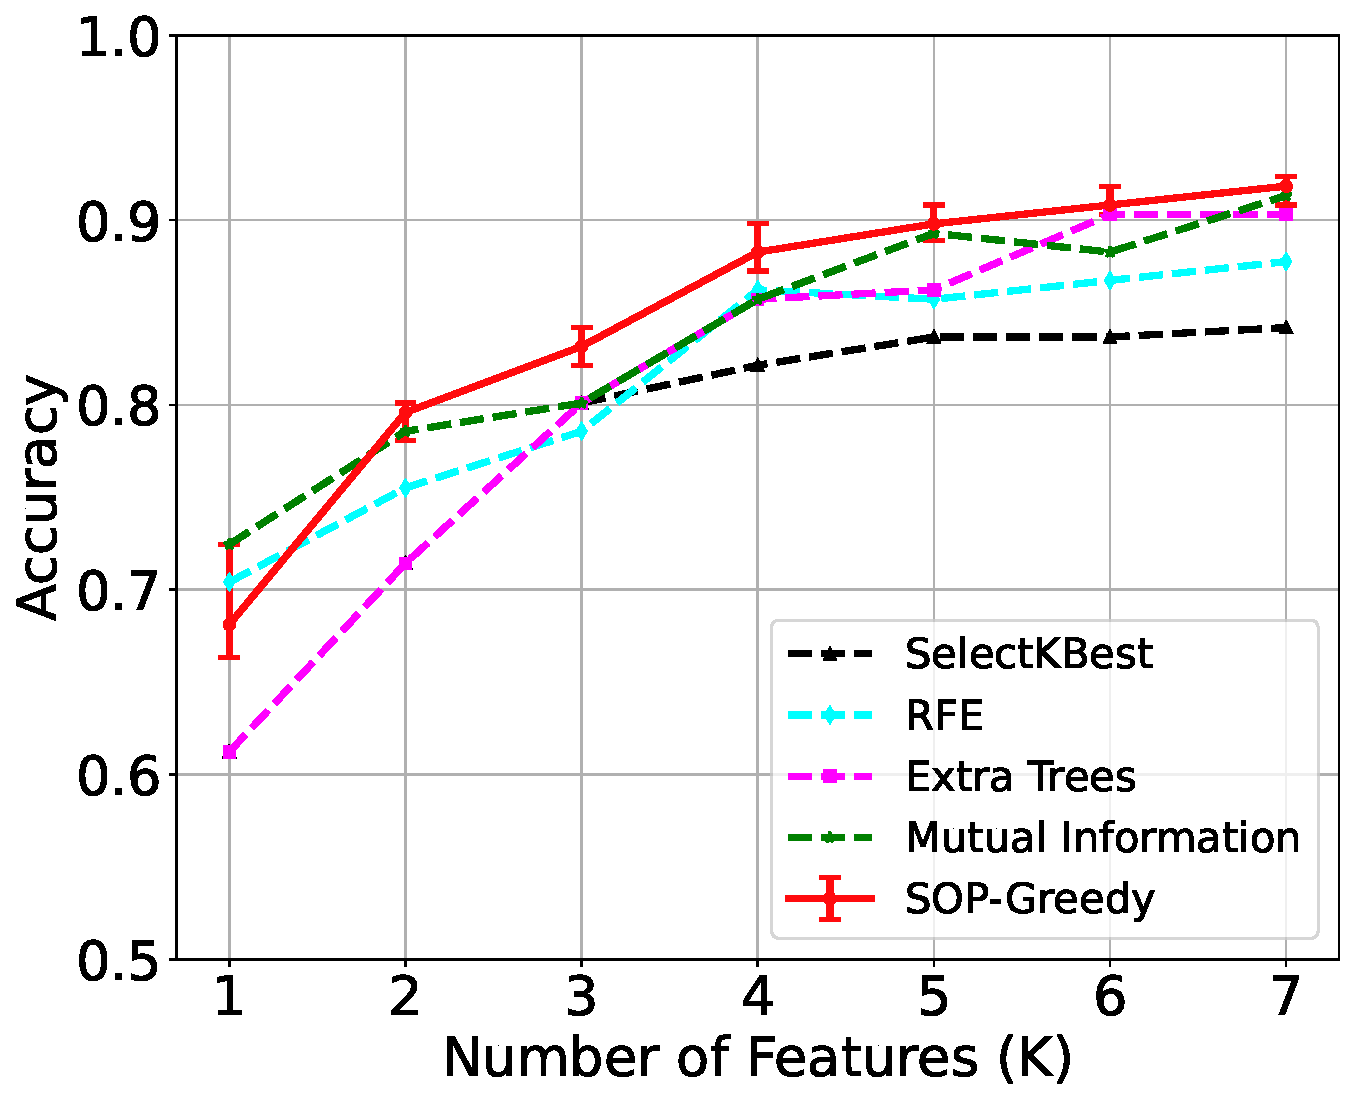
\includegraphics[width=\linewidth]{Figures/experiment 1/predictive_performance_airline3.pdf}
        %\\{\tiny (a)}
        \label{fig:airline_performance}
    \end{minipage}\hfill
    % Second figure
    \begin{minipage}{0.24\textwidth}
        \centering
        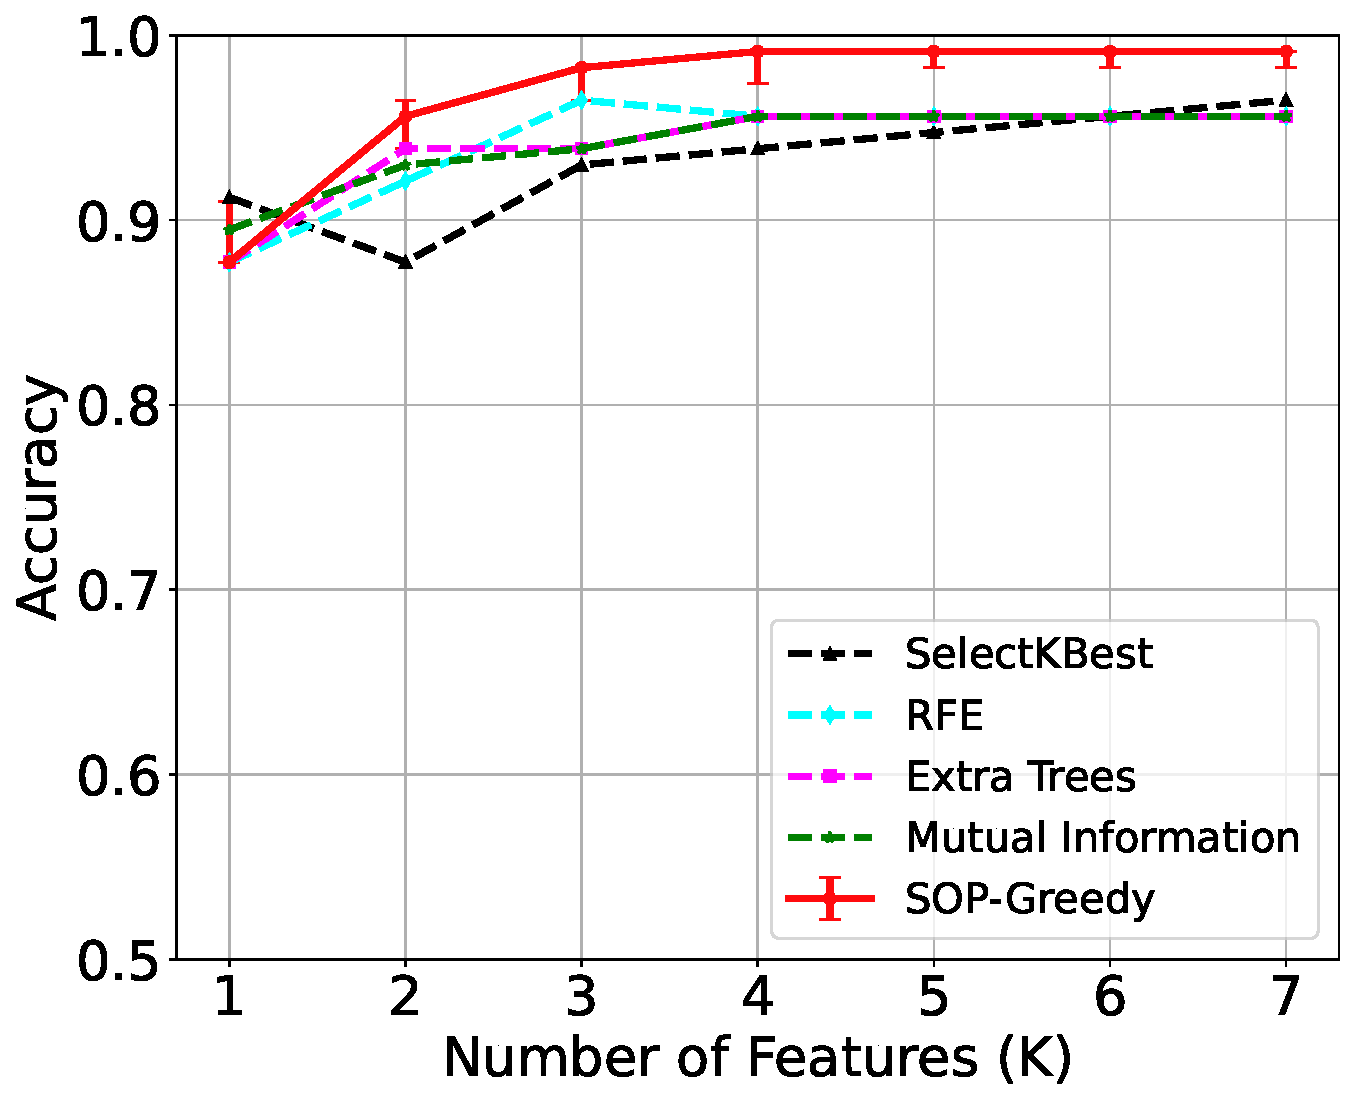
\includegraphics[width=\linewidth]{Figures/experiment 1/predictive_performance3.pdf}
        %\\{\tiny (b)}
        \label{fig:cancer_performance}
    \end{minipage}
    \hfill
    % Third figure
    \begin{minipage}{0.24\textwidth}
        \centering
        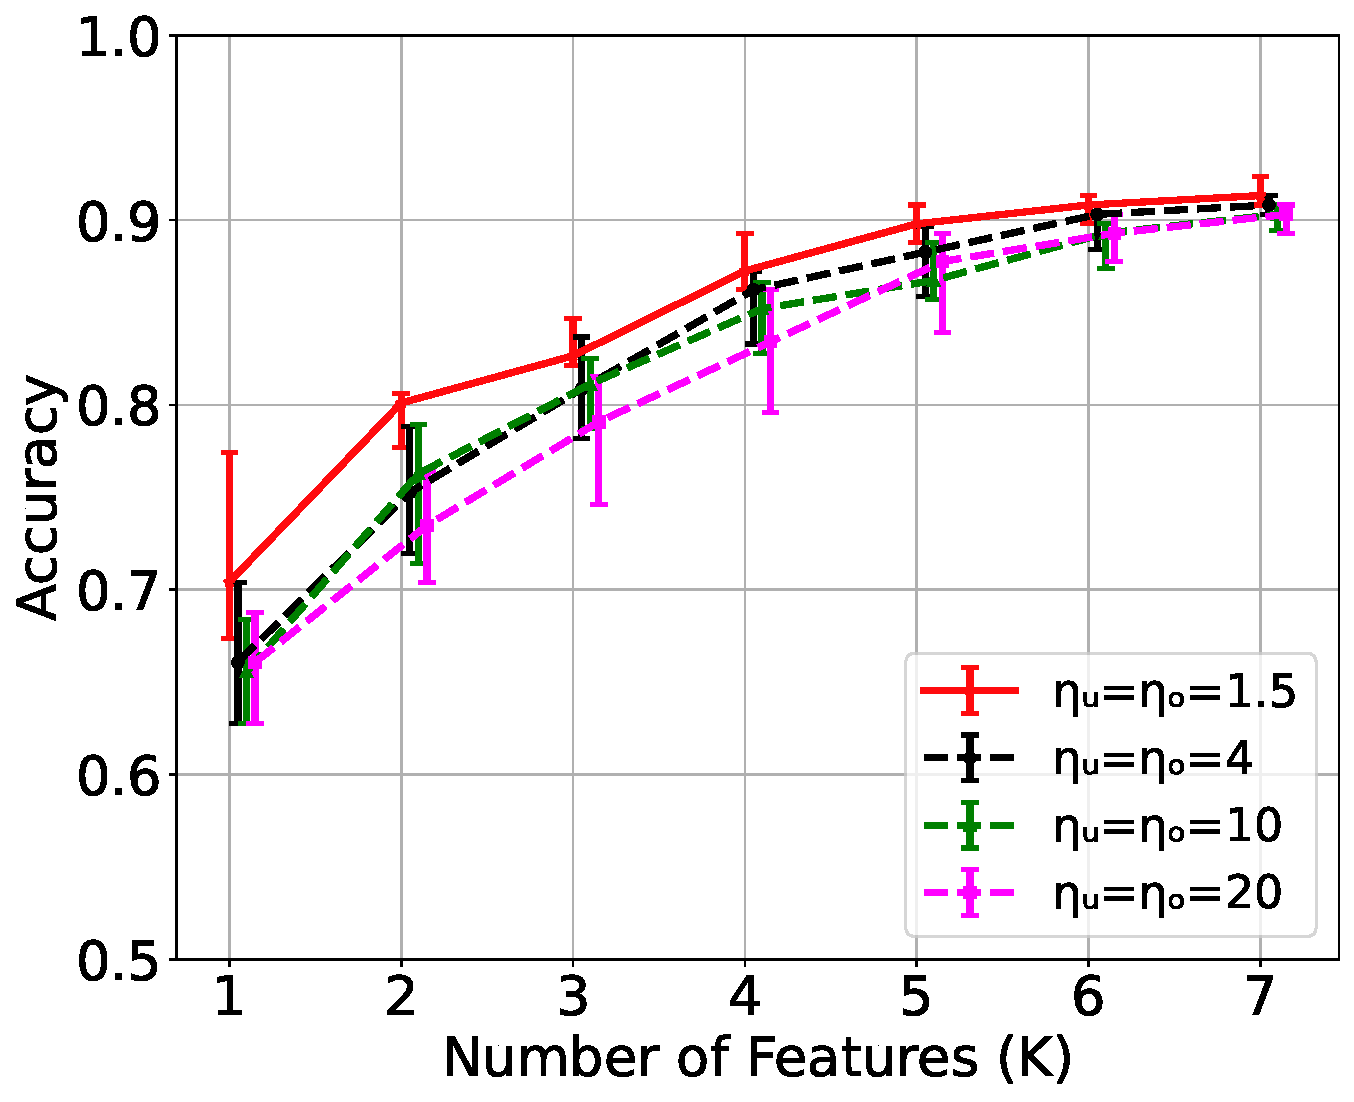
\includegraphics[width=\linewidth]{Figures/experiment 1/eta_airline_performance4.pdf}
        %\\{\tiny (c)}
        \label{fig:eta_airline}
    \end{minipage}
    \hfill
    % Fourth figure
    \begin{minipage}{0.24\textwidth}
        \centering
        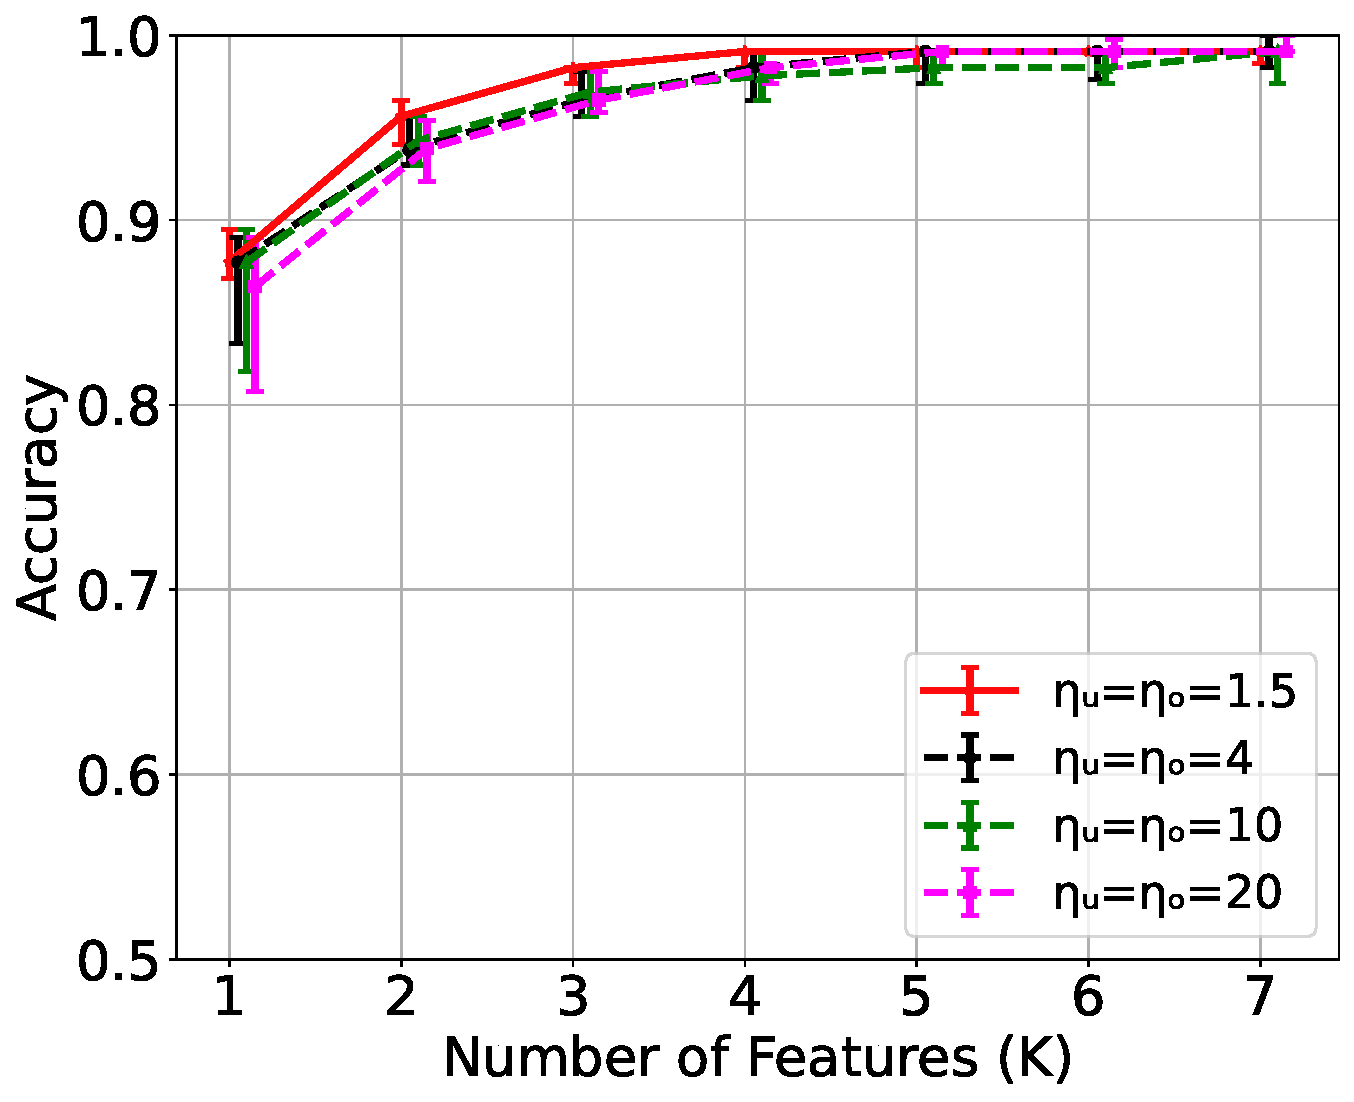
\includegraphics[width=\linewidth]{Figures/experiment 1/eta_cancer_performance2.pdf}
        %\\{\tiny (d)}
        \label{fig:eta_cancer}
    \end{minipage}

    \caption{The oos accuracy of Submodular Optimization Predictive Greedy (SOP-Greedy), with $R = 1$ and $\eta_o = \eta_u = 1.5$, against four benchmarks and under different prediction errors. From left to right, the first two figures are under an increasing $K$ for the airline passenger satisfaction and breast cancer datasets. The last two are the performance of SOP-Greedy under an increasing $\eta$, from 2.25 to 400, for the two tasks.}
    \label{fig:experiment1-performance}
    \vspace{-10pt}
\end{figure*}

% \footnote{https://anonymous.4open.science/r/SubmodularExperiment-DB09/}}
\begin{figure}
    \centering
    % First figure
    \begin{minipage}{0.42\textwidth}
        \centering
        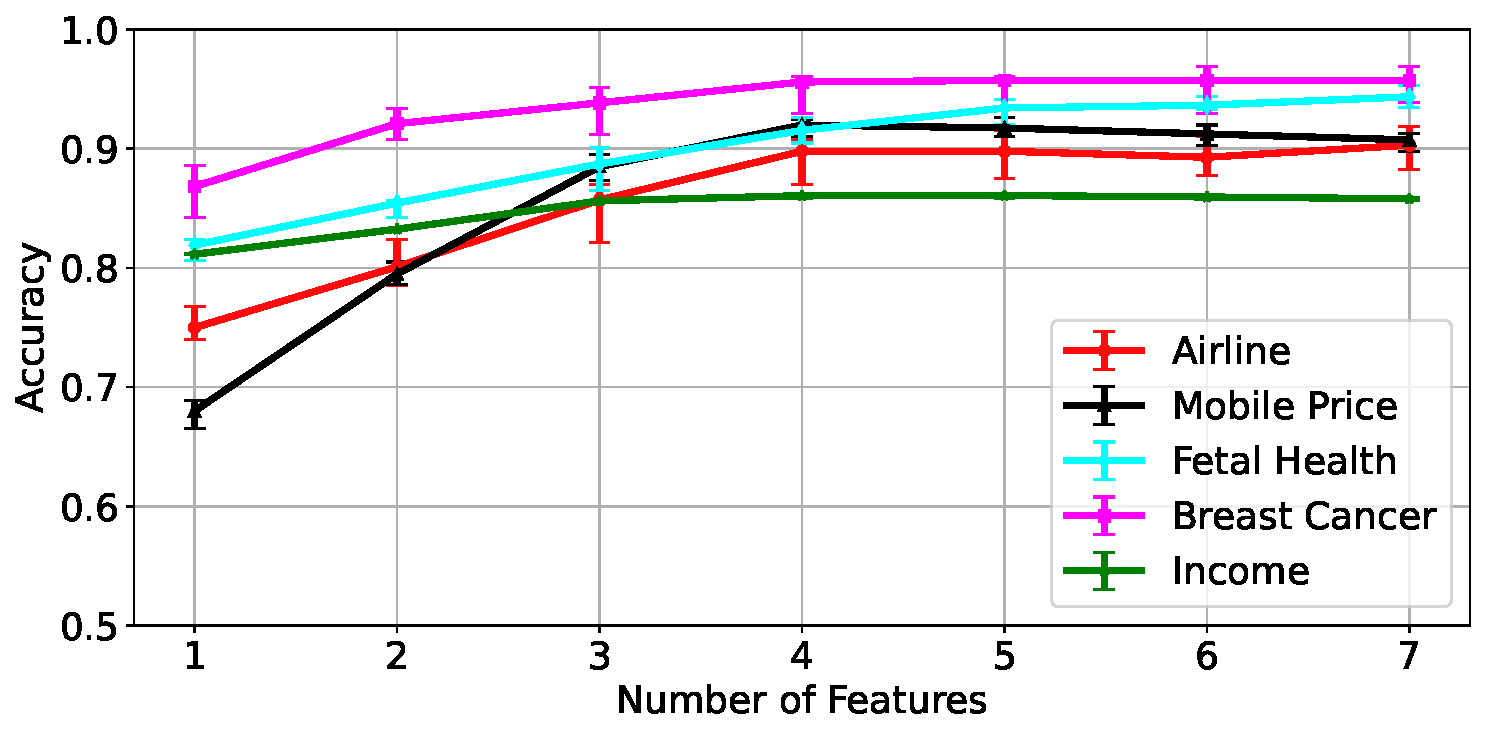
\includegraphics[width=\linewidth]{Figures/experiment 1/combined_submodular_proof (1).pdf}
        %\\{\tiny (a)}
    \end{minipage}\hfill
    
    \caption{Empirical evidence of the approximate submodularity for oos accuracy as a function of the number of features verified on five real-world classification datasets \cite{Salini2024,Kalaivani2021,Chakraborty2020}. We run a greedy feature selection and measure the additivity of each feature. The overall accuracy increases when features are added with clear diminishing returns.}
    \label{fig:submod}
    \vspace{-12pt}
\end{figure}





\begin{figure}[t]
    \centering
    % First figure
    \begin{minipage}{0.45\textwidth}
        \centering
        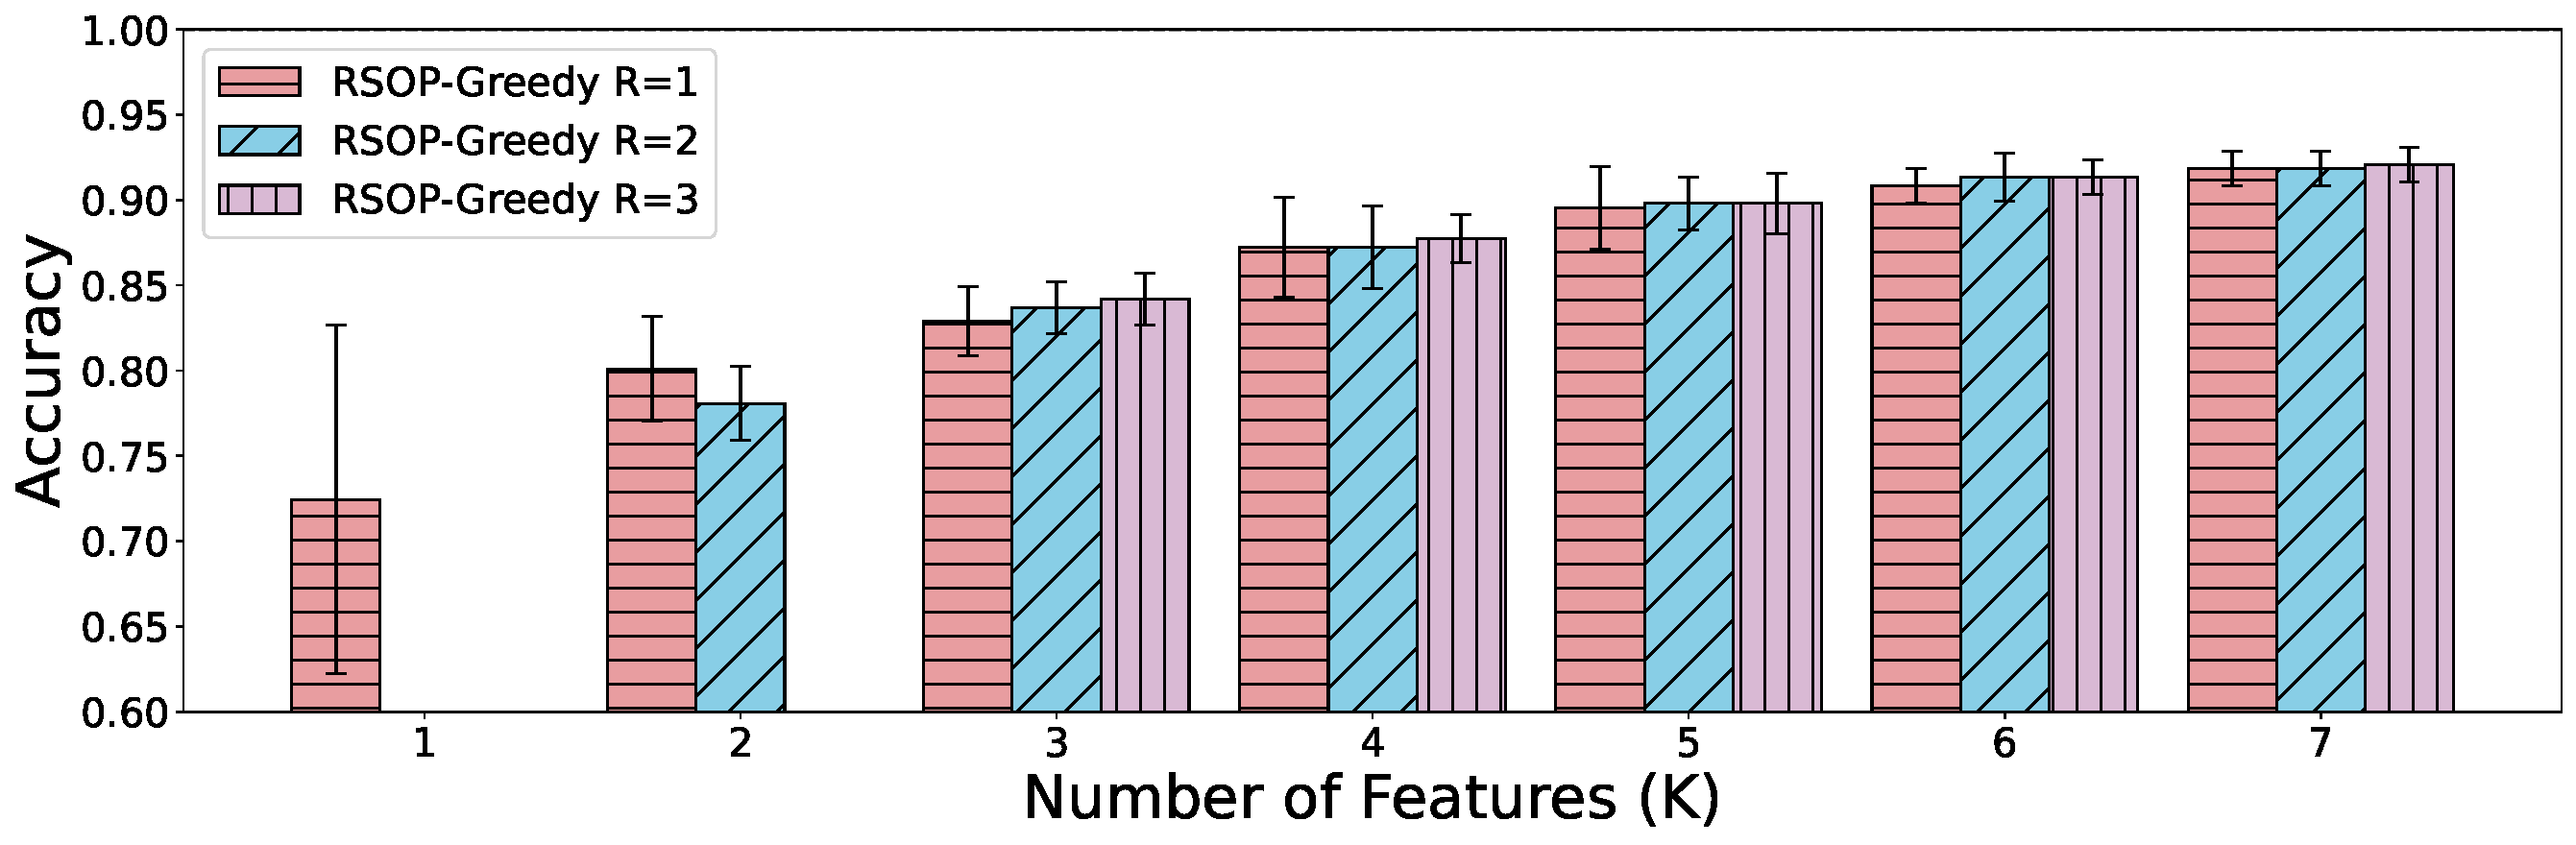
\includegraphics[width=\linewidth]{Figures/experiment 1/r_airline.pdf}
        %\\{\tiny (a)}
        \label{fig:airline_performance_R_step}
    \end{minipage}\hfill
    % Second figure
    \begin{minipage}{0.44\textwidth}
        \centering
        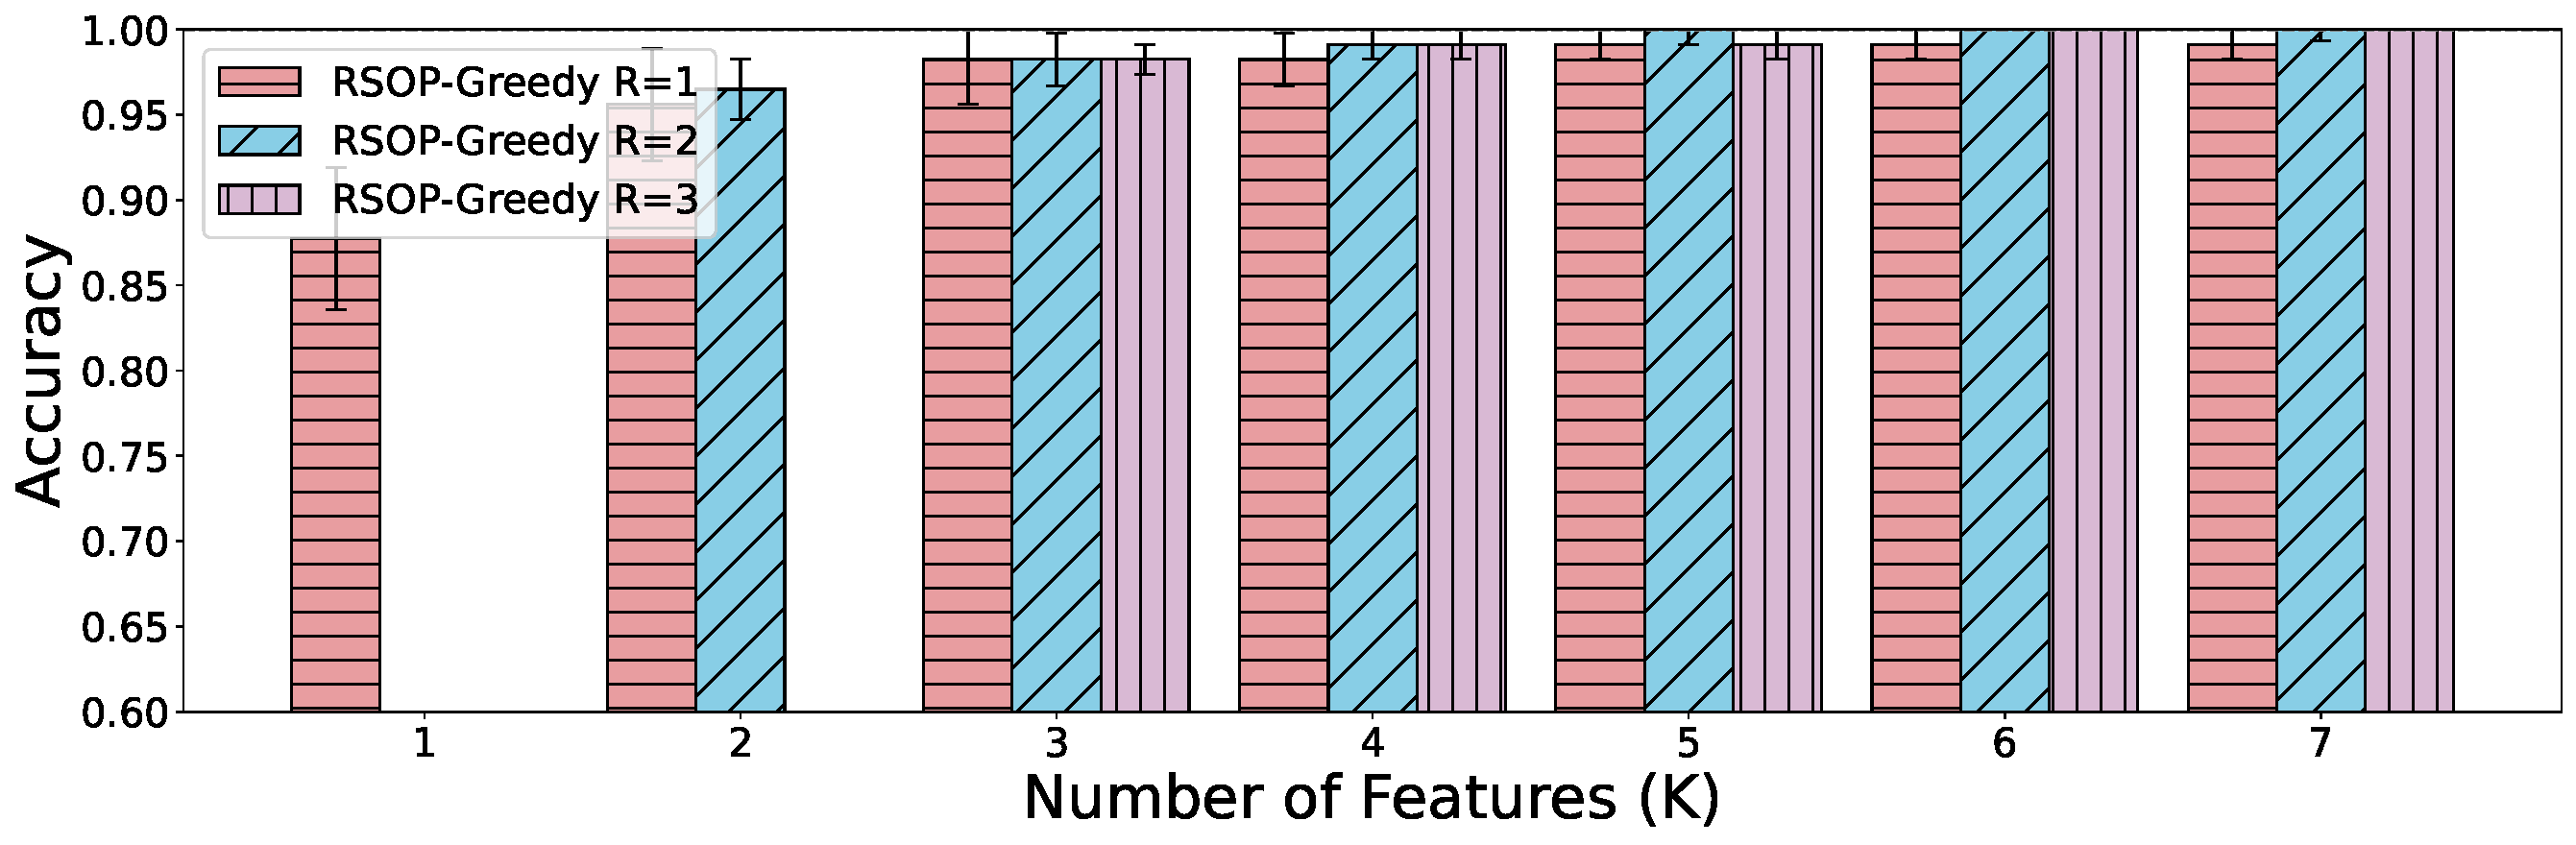
\includegraphics[width=\linewidth]{Figures/experiment 1/r_cancer.pdf}
        %\\{\tiny (b)}
        \label{fig:predictive_performance}
    \end{minipage}

    \caption{The oos accuracy of the R-step Greedy (RSOP-Greedy) with $R = 1, 2, 3$ and $\eta_o = \eta_u = 1.5$. From left to right, the figures present the accuracy with different $K$ for the airline and breast cancer datasets.}
    \label{fig:experiment2-R-step}
    \vspace{-6pt}
\end{figure}

\vspace{-10pt}
\subsection{ML feature selection} \label{subsec:feature-selection}


% Pose the application as submodular optimization
Supervised learning aims at predictive models that perform well on \textit{out-of-sample (oos)} data. Given training data $\boldsymbol{X}$ with $n$ feature columns labeled as $1, ..., n$ and a target vector $y$, our task is to find features $S \subseteq [n]$, subject to $|S| \leq K$ for a given $K$, for model $h(\boldsymbol{Y}[S]; \boldsymbol{\theta})$, where $S \subseteq [n]$, $\boldsymbol{Y}[S]$ denotes data $\boldsymbol{Y}$ with columns $S$, and $\boldsymbol{\theta}$ the model parameters depending on $S$. The model's performance is defined by function $\mathcal{L}$ on some oos data $\boldsymbol{Z}$ and a target vector $w$, denoted by $\mathcal{L}(h(\boldsymbol{Z}[S]; \boldsymbol{\theta}), w)$. We assume a given training process $p$ that determines $\boldsymbol{\theta}$ given $\boldsymbol{X}$, $y$, and $S$. The ML feature selection problem can be cast as: 
\[ \max_{S \subseteq [n]}\{ \mathcal{L}(h(\boldsymbol{Z}[S]; p(\boldsymbol{X}, y, S)), w): |S| \leq K\} \]
where $\mathcal{L}$, $h$, $p$, $\boldsymbol{X}$, $y$, and $K$ are known, $\boldsymbol{Z}$ and $w$ are not, and $S$ is the decision variable. Let $f(S) = \mathcal{L}(h(\boldsymbol{Z}[S]; p(\boldsymbol{X}, y, S)), w)$. Function $f$ may not be strictly submodular, but has observed diminishing gains in adding features due to feature correlation \cite{wei2014submodular}. This empirical observation is verified in various learning tasks shown in Figure \ref{fig:submod}. Thus, $f$ is assumed to be submodular. We cannot access $f$, but we assume a predictor $\tilde{f}$ for $f$ is accessible, allowing us to query $\tilde{d}_B(A)$ for any $A, B \subseteq [n]$.
% Give experimental set-up: how our algorithm is implemented, what are the benchmarks

\begin{table}[ht!]
\centering
\caption{Empirical ratios of RSOP-Greedy with different $R$ (estimated assuming $\mathrm{OPT}=1$) in the airline dataset and their theoretical bounds ($\eta=2.25$).}
\label{tab:airline-r-steps-theo}
\begin{tabular}{c|ccccccc}
\hline\hline
\textbf{R} 
& \textbf{K=1} & \textbf{K=2} & \textbf{K=3} & \textbf{K=4} & \textbf{K=5} & \textbf{K=6} & \textbf{K=7}\\
\hline
{\textbf{1}} 
  & 0.725 & 0.801 & 0.829 & 0.872 & 0.895 & 0.908 & 0.918 \\[-3pt]
  & (0.444) & (0.395) & (0.382) & (0.376) & (0.371) & (0.369) & (0.366) \\
{\textbf{2}}
  & ---   & 0.781 & 0.837 & 0.872 & 0.898 & 0.913 & 0.918 \\[-3pt]
  & (0.444) & (0.444) & (0.395) & (0.395) & (0.382) & (0.382) & (0.376) \\
{\textbf{3}}
  & ---   & ---   & 0.842 & 0.878 & 0.898 & 0.913 & 0.921 \\[-3pt]
  & (0.444) & (0.444) & (0.444) & (0.395) & (0.395) & (0.395) & (0.382) \\
\hline\hline
\end{tabular}
\vspace{-5pt}
\end{table}

\begin{table}[ht!]
\centering
\caption{Empirical ratios of RSOP-Greedy in the breast cancer dataset and their theoretical bounds ($\eta=2.25$).}
\label{tab:breast-r-steps-theo}
\begin{tabular}{c|ccccccc}
\hline\hline
\textbf{R} 
& \textbf{K=1} & \textbf{K=2} & \textbf{K=3} & \textbf{K=4} & \textbf{K=5} & \textbf{K=6} & \textbf{K=7}\\
\hline
{\textbf{1}} 
  & 0.877 & 0.965 & 0.983 & 0.991 & 0.991 & 0.991 & 0.991 \\[-3pt]
  & (0.444) & (0.395) & (0.382) & (0.376) & (0.371) & (0.369) & (0.366) \\
{\textbf{2}}
  & ---    & 0.956 & 0.991 & 0.991 & 0.983 & 1.000 & 1.000 \\[-3pt]
  & (0.444) & (0.444) & (0.395) & (0.395) & (0.382) & (0.382) & (0.376) \\
{\textbf{3}}
  & ---    & ---    & 0.974 & 0.991 & 1.000 & 1.000 & 1.000 \\[-3pt]
  & (0.444) & (0.444) & (0.444) & (0.395) & (0.395) & (0.395) & (0.382) \\
\hline\hline
\end{tabular}
%\vspace{-12pt}
\end{table}

\begin{figure*}[t!]
    \centering
    % First figure
    \begin{minipage}{0.245\textwidth}
        \centering
        
\includegraphics[width=\linewidth]{Figures/experiment 2/new/n_twt.pdf}
        \label{fig:2stp_twt}
    \end{minipage}\hfill
    % Second figure
    \begin{minipage}{0.245\textwidth}
        \centering
        
\includegraphics[width=\linewidth]{Figures/experiment 2/new/n_rdt.pdf}
        \label{fig:2stp_rdt}
    \end{minipage}
    \hfill
    % Third figure
    \begin{minipage}{0.245\textwidth}
        \centering
        
\includegraphics[width=\linewidth]{Figures/experiment 2/new/n_fb1.pdf}
        \label{fig:2stp_fb1}
    \end{minipage}
    \hfill
    % Fourth figure
    \begin{minipage}{0.245\textwidth}
        \centering
        
\includegraphics[width=\linewidth]{Figures/experiment 2/new/n_fb2.pdf}
        \label{fig:2stp_fb2}
    \end{minipage}

    \caption{Performance ratio with an increasing $K$. We retain 1000 nodes for each dataset for reasonable run-time of RSOP-Greedy. 
    % Results on the full networks (excluding RSOP-Greedy) are in the Appendix E.
    %\ref{appendix:large-scale}.
    }
    \label{fig:2stp}
\end{figure*}






\begin{figure*}[t!]
    \centering
    % First figure
    \begin{minipage}{0.19\textwidth}
        \centering
        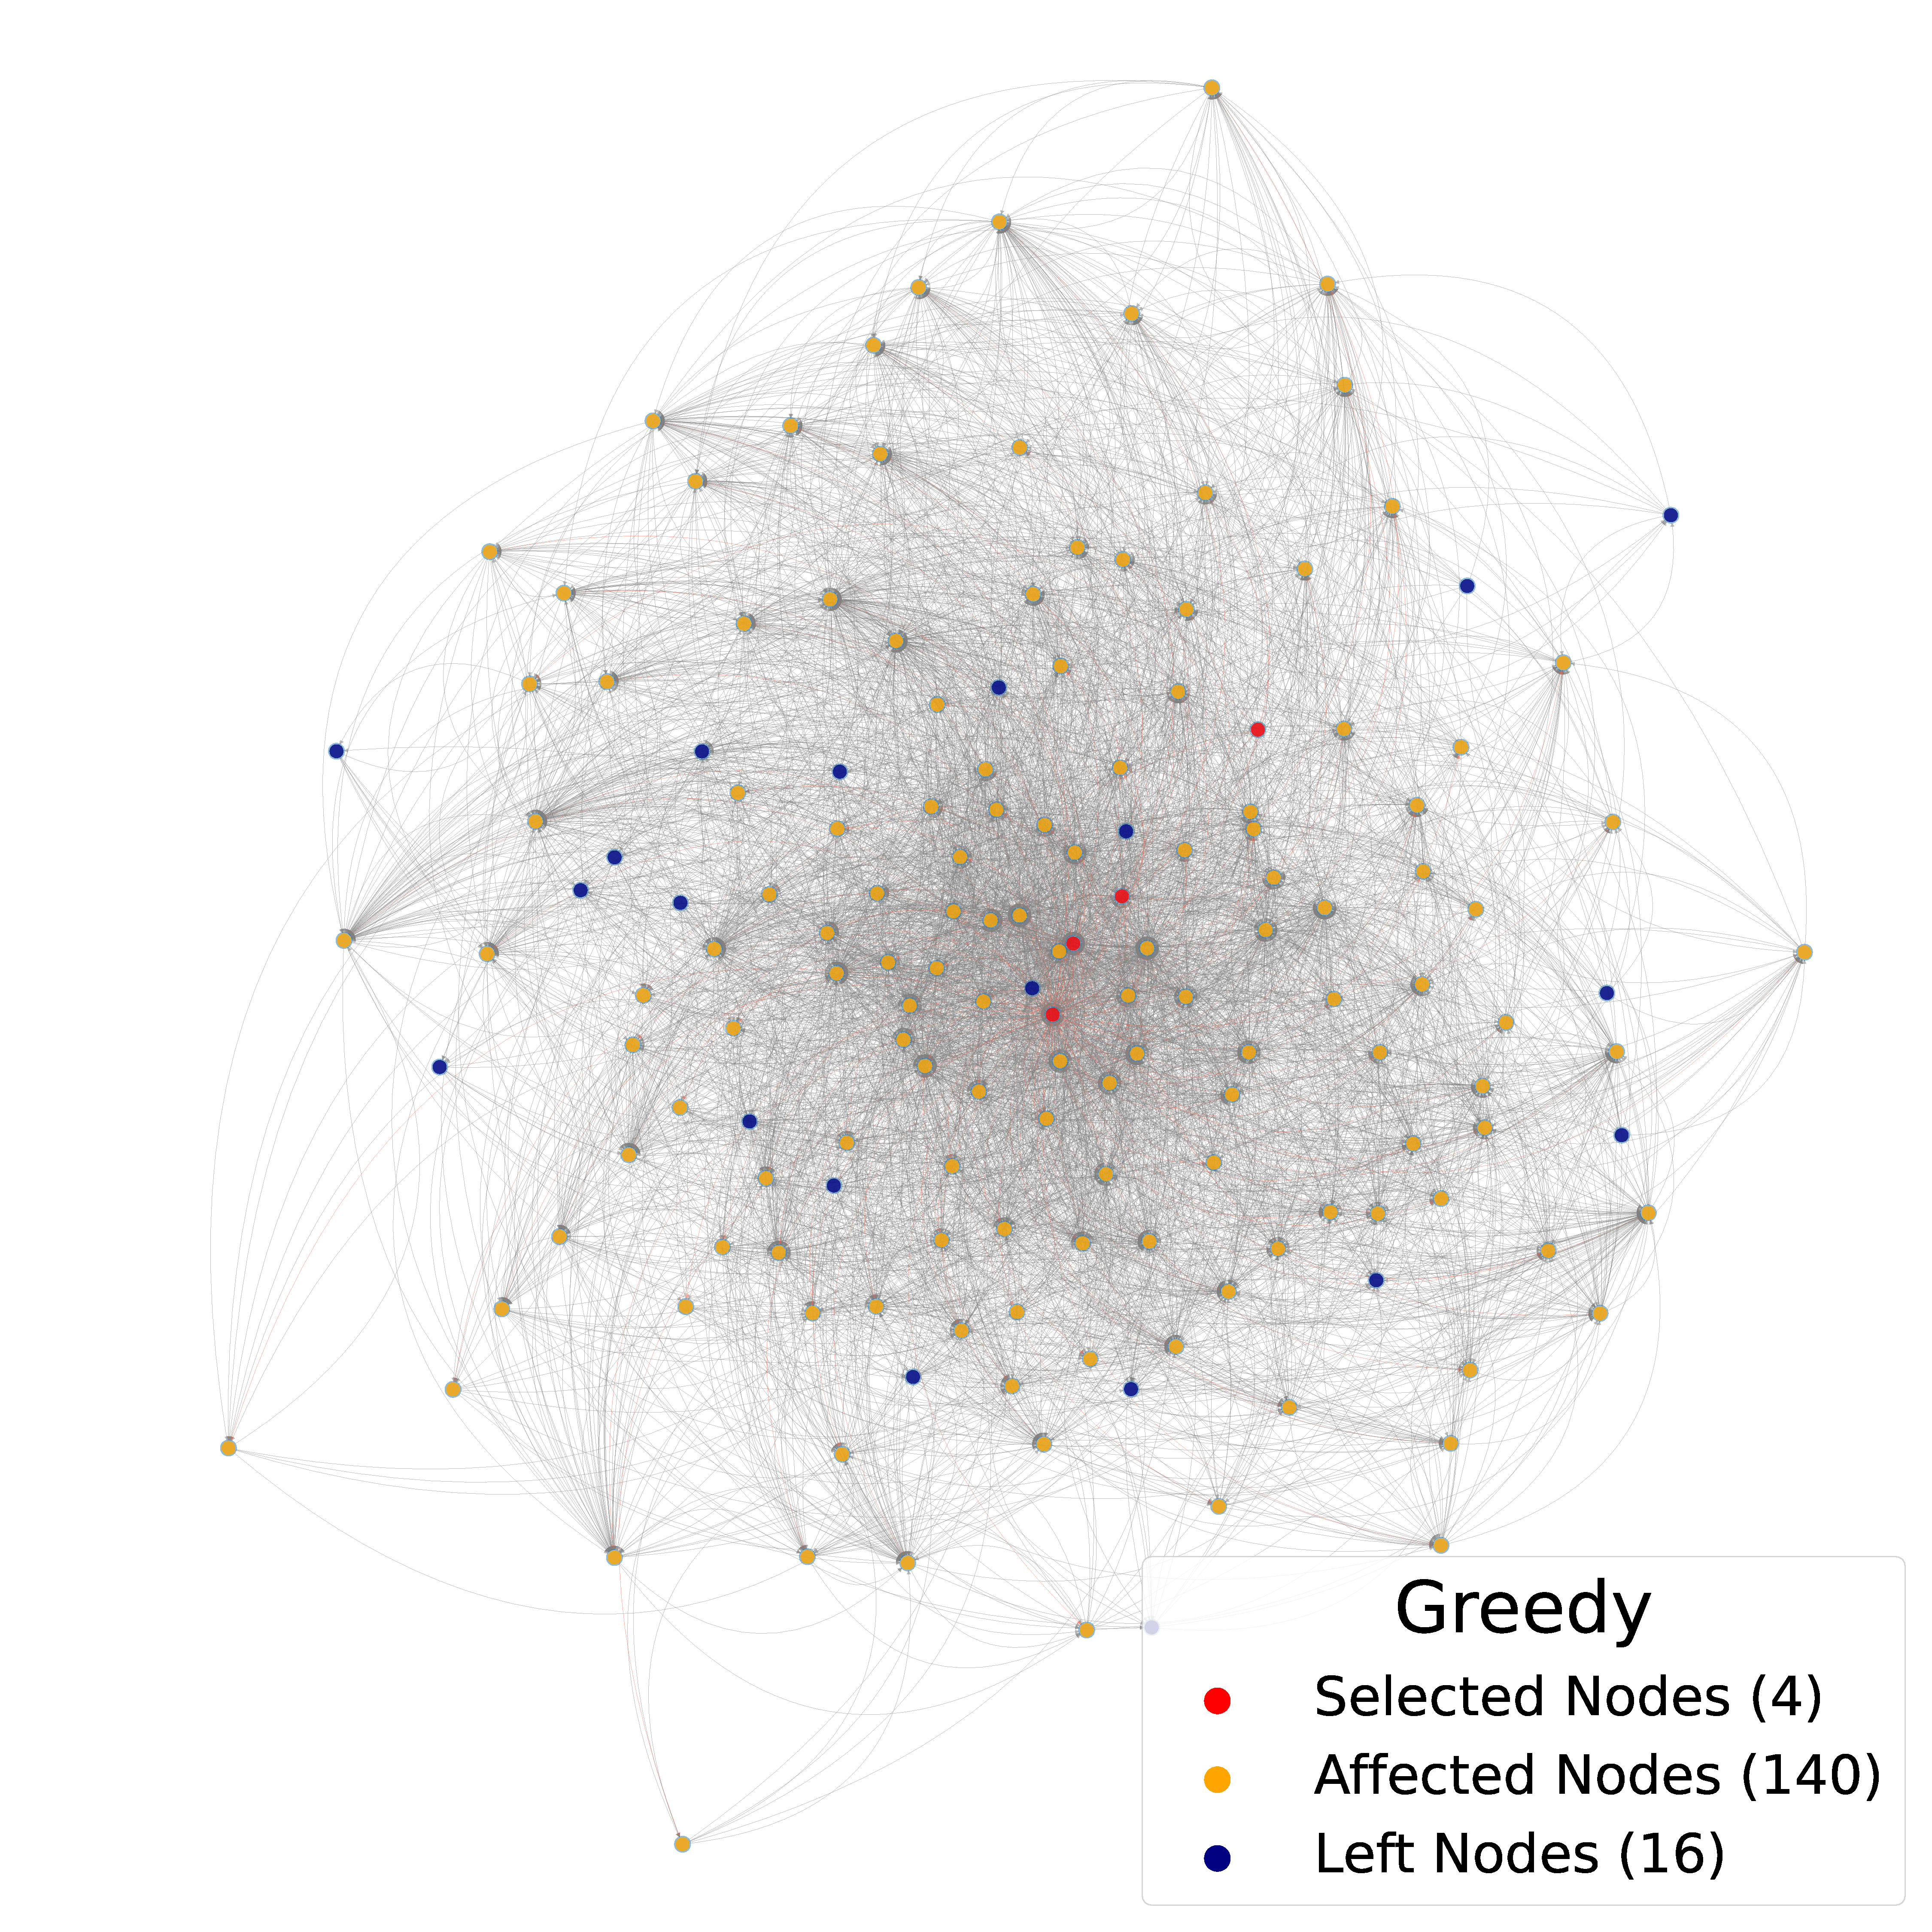
\includegraphics[width=\linewidth]{Figures/GraphExperiment/Network/plot_Greedy.pdf}
        %\\{\tiny Greedy}
        \label{fig:g}
    \end{minipage}%\hspace{0.005\textwidth}
    \hfill
    % Second figure
    \begin{minipage}{0.19\textwidth}
        \centering
        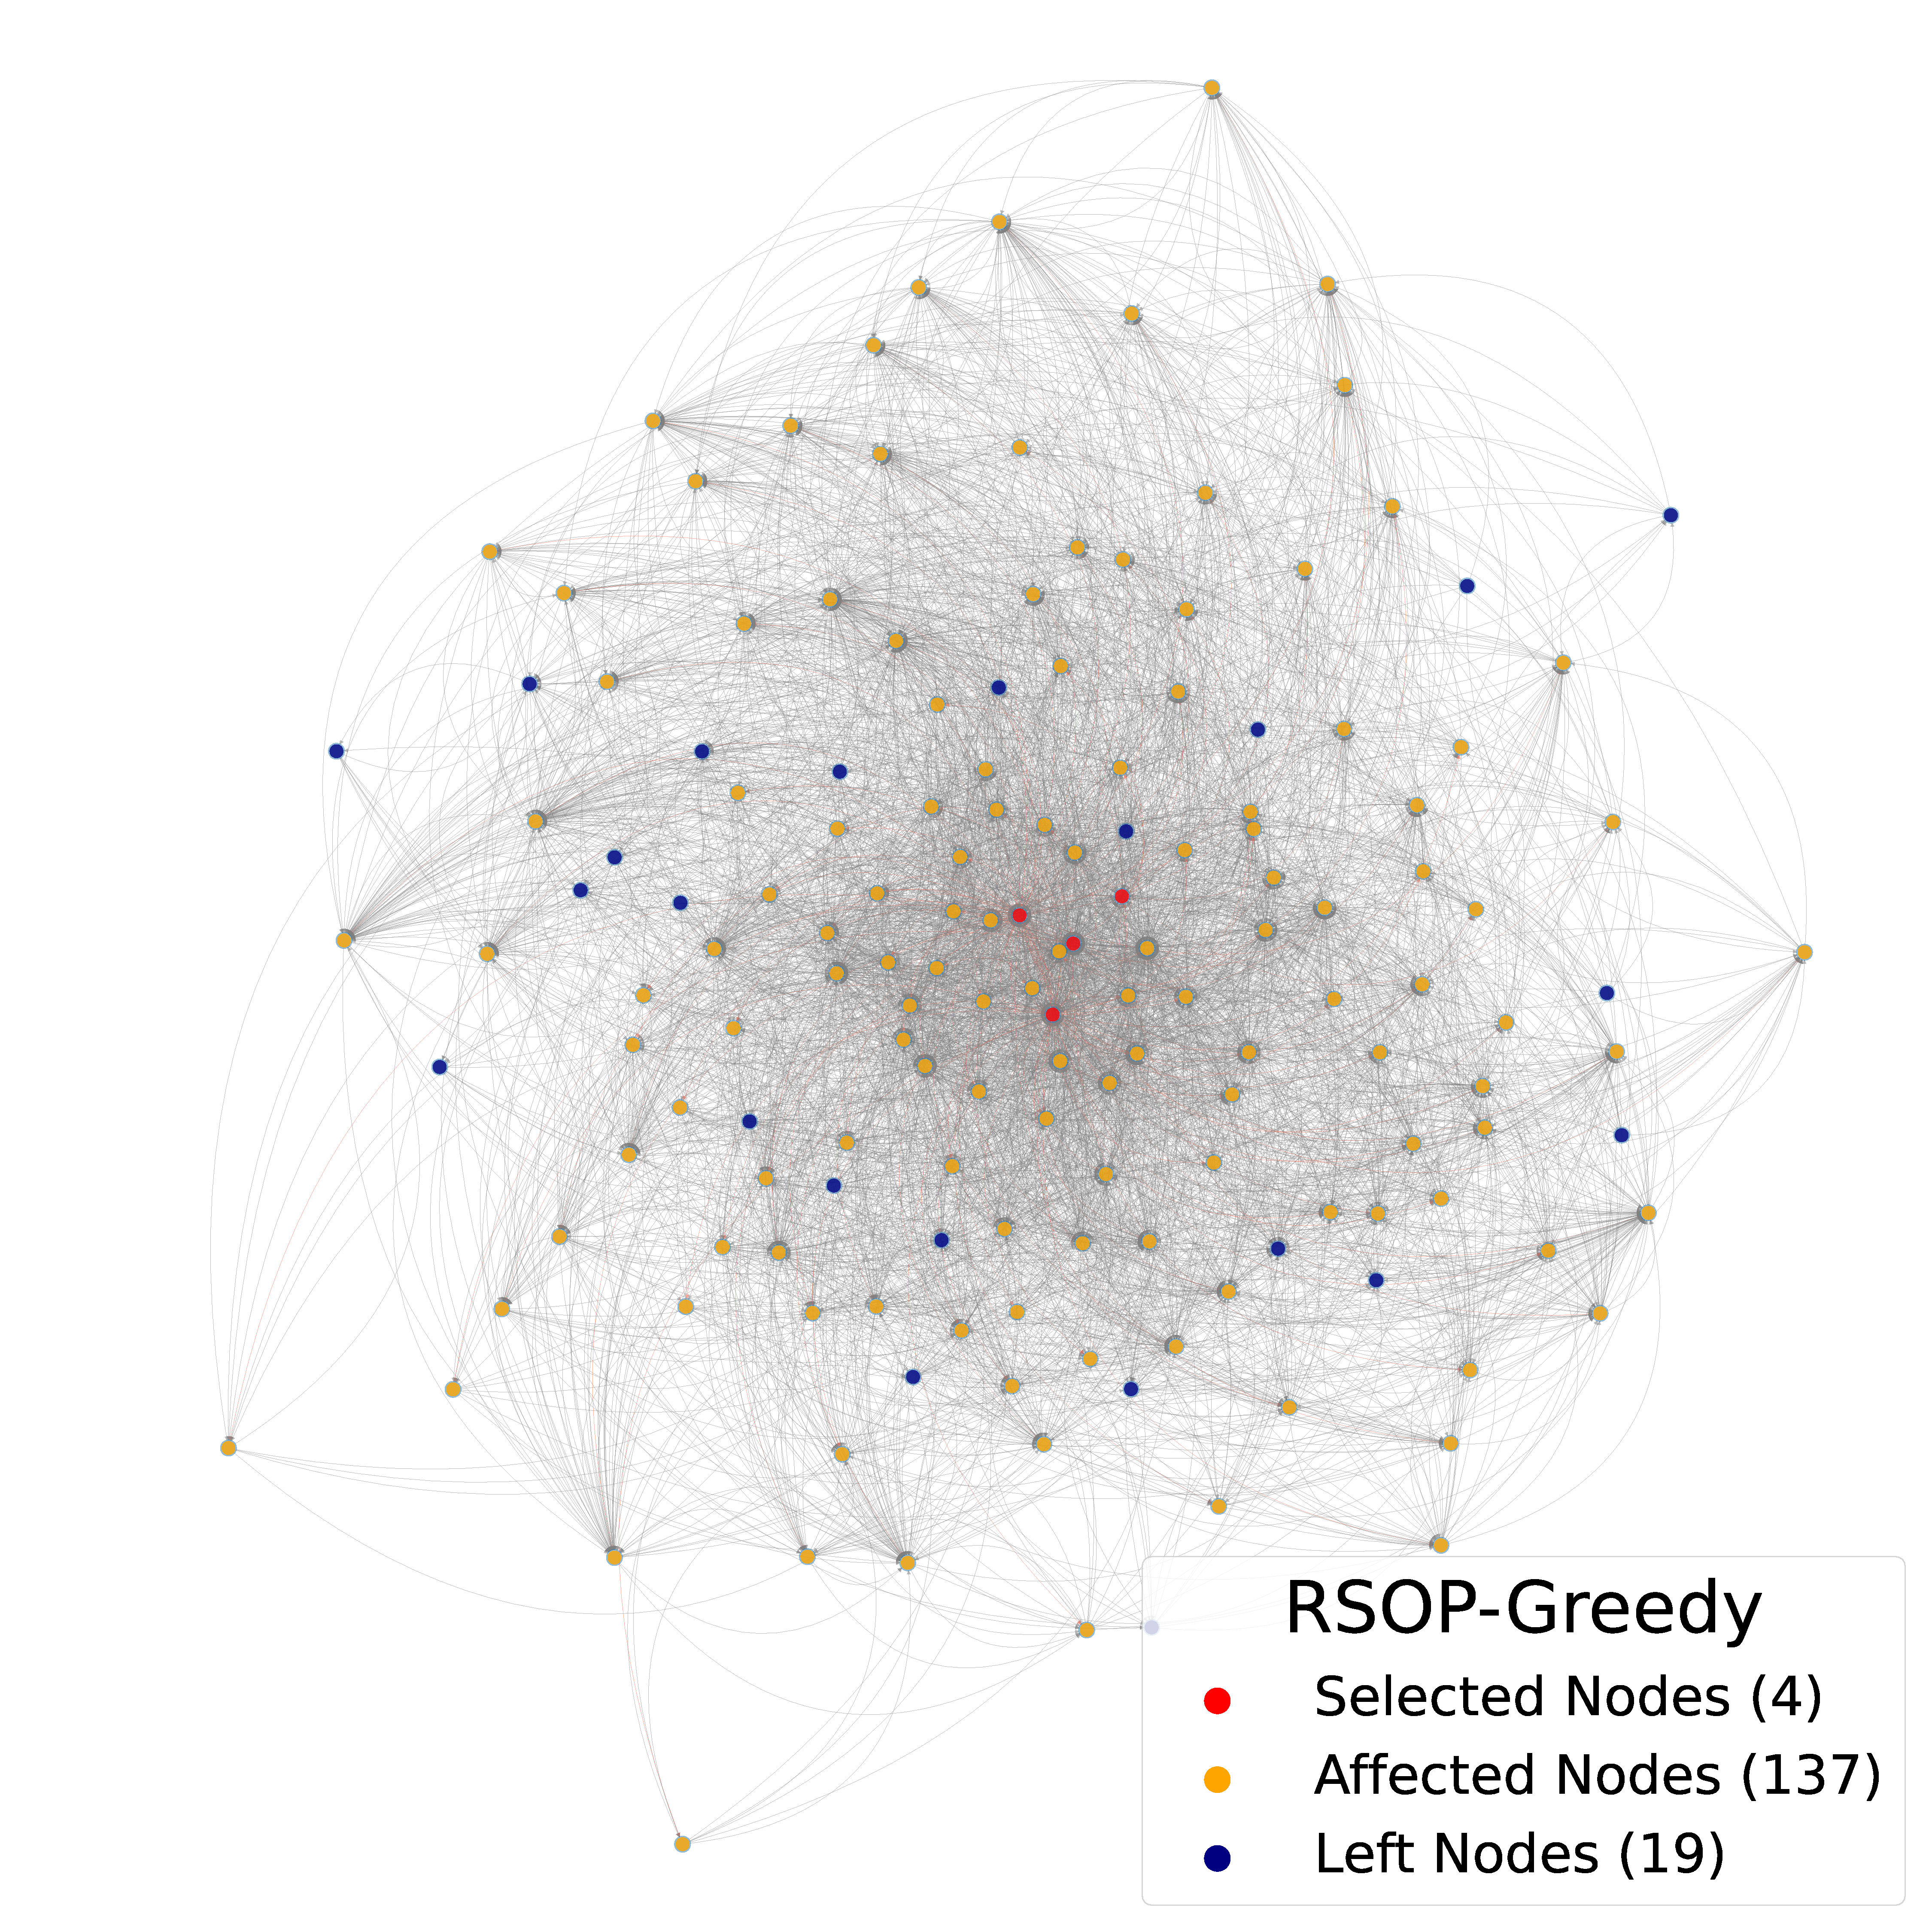
\includegraphics[width=\linewidth]{Figures/GraphExperiment/Network/plot_RSOP-Greedy.pdf}
        %\\{\tiny SOP-Greedy}
        \label{fig:sop}
    \end{minipage}%\hspace{0.005\textwidth}
    \hfill
    % Third figure
    \begin{minipage}{0.19\textwidth}
        \centering
        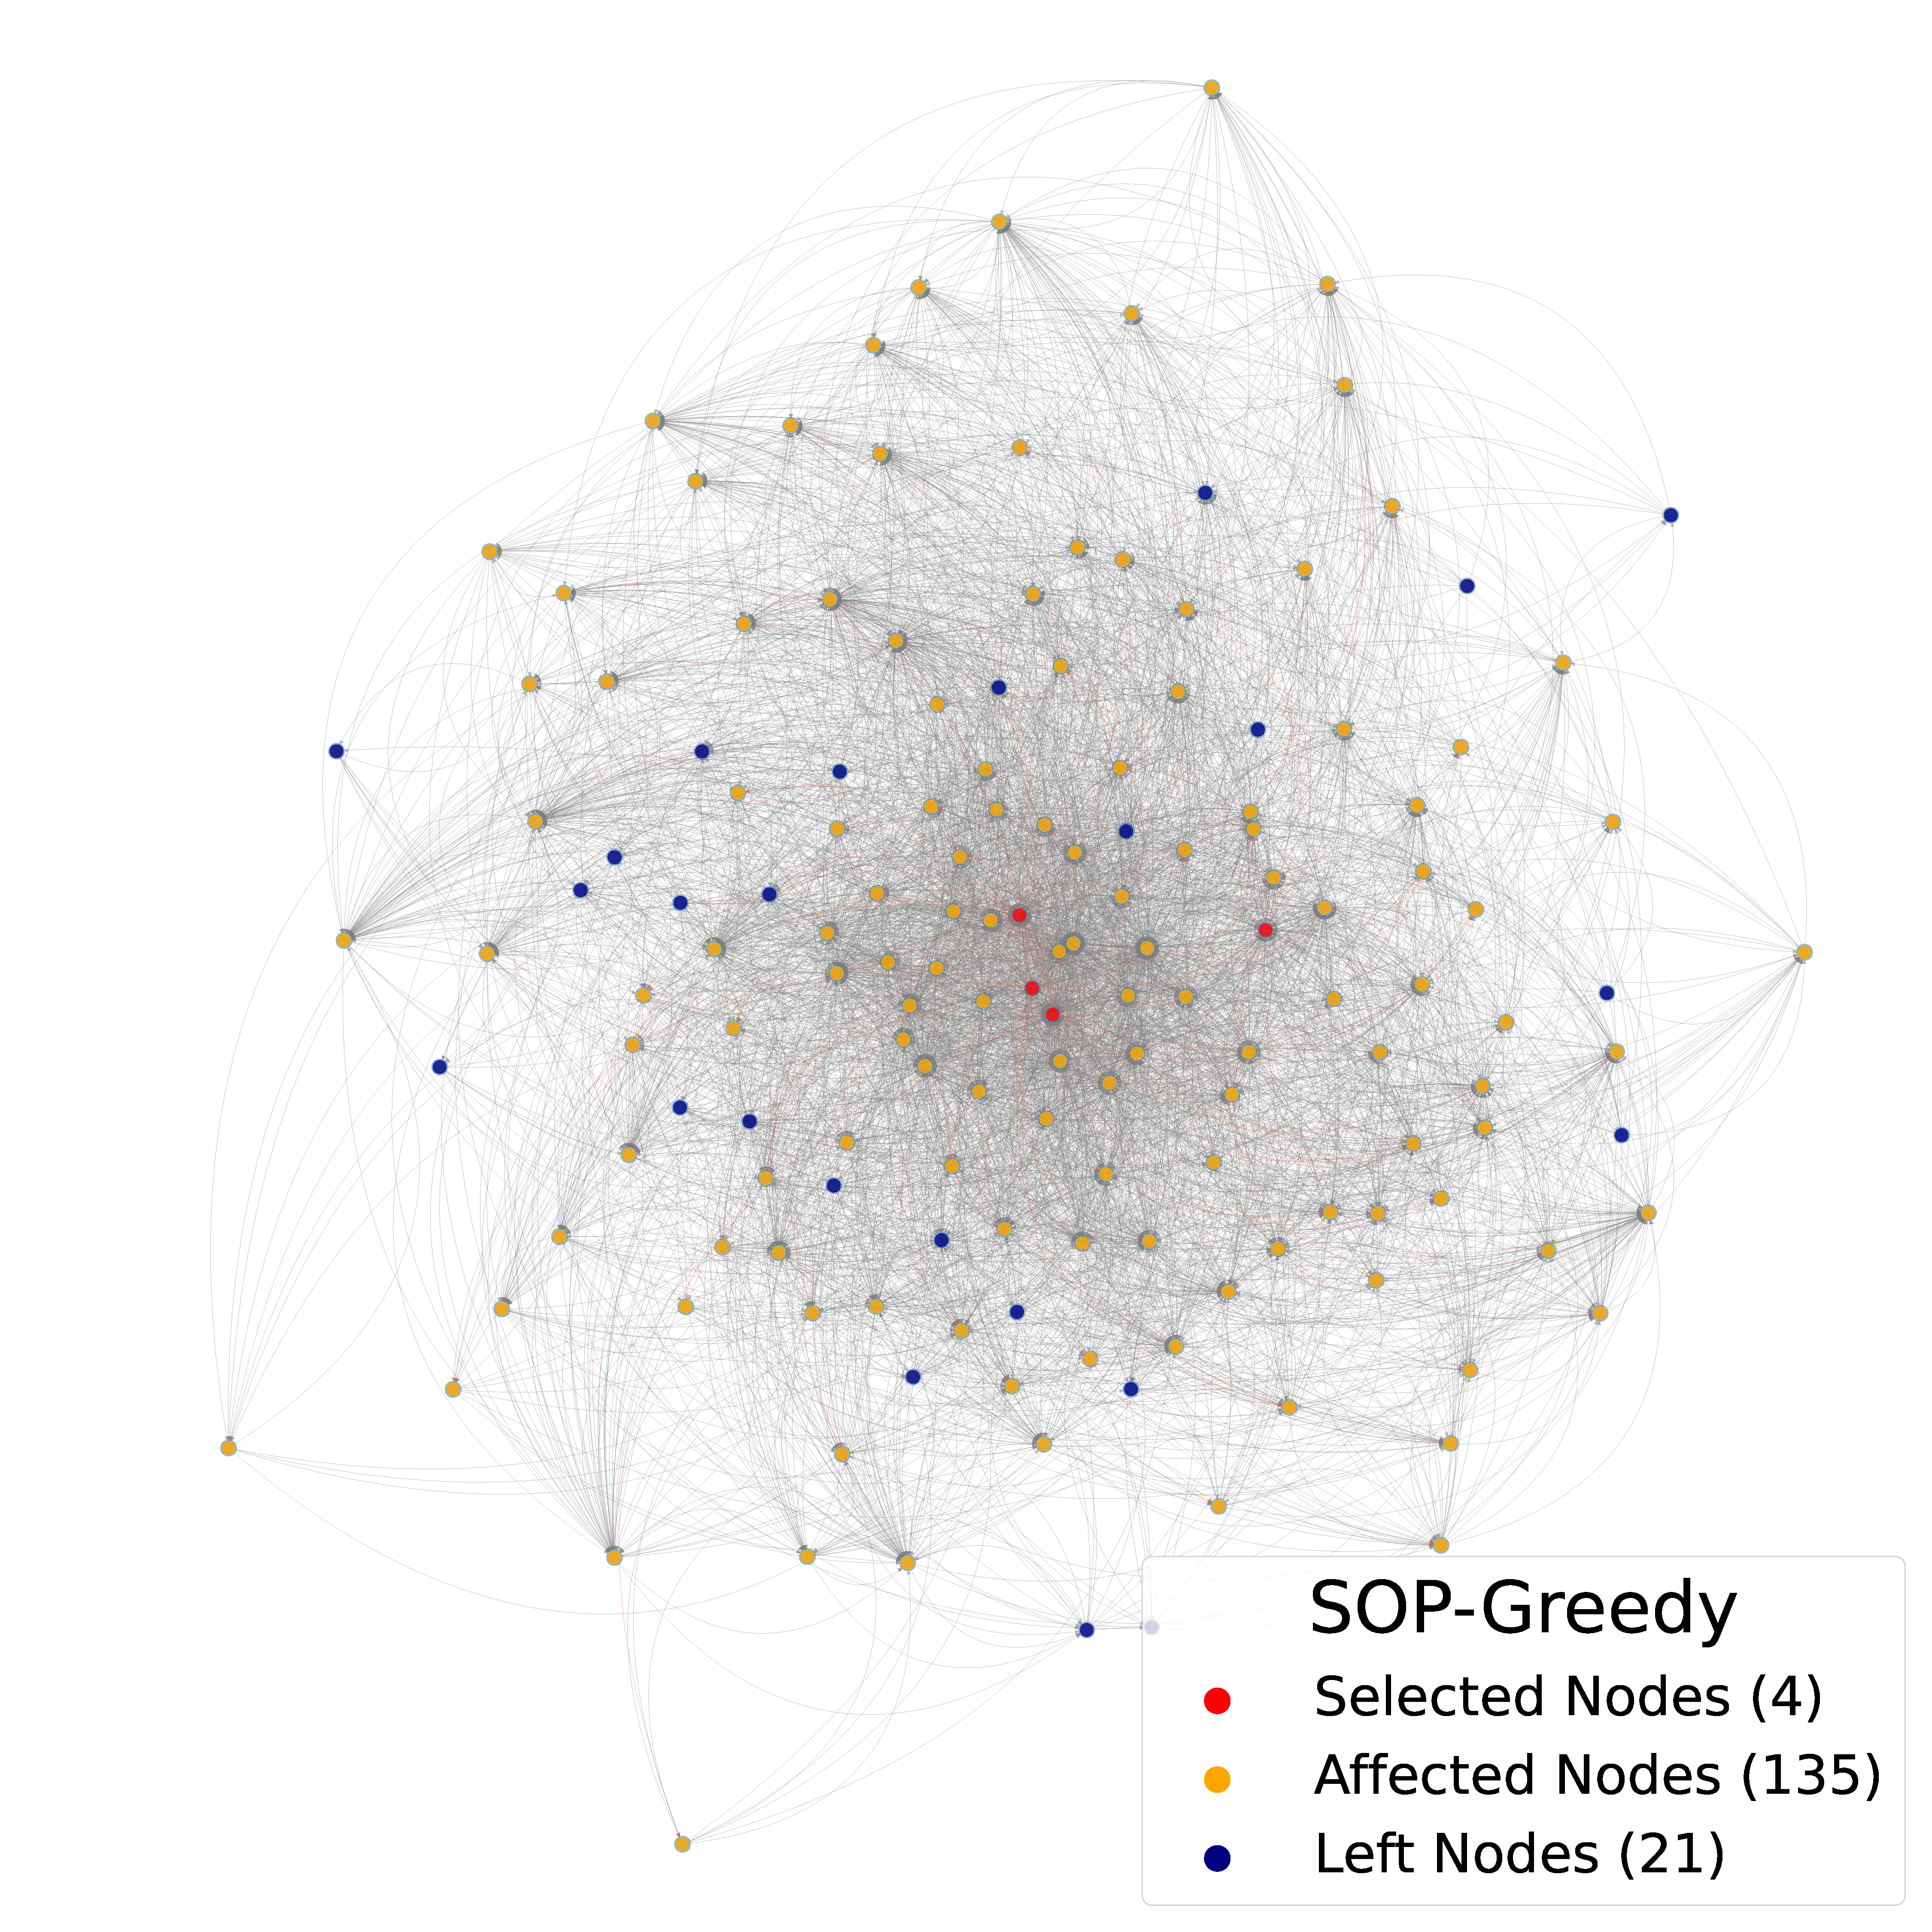
\includegraphics[width=\linewidth]{Figures/GraphExperiment/Network/plot_SOP-Greedy.pdf}
        %\\{\tiny RSOP-Greedy ($R = 2$)}
        \label{fig:rsop}
    \end{minipage}%\hspace{0.005\textwidth}
    \hfill
    % Fourth figure
    \begin{minipage}{0.19\textwidth}
        \centering
        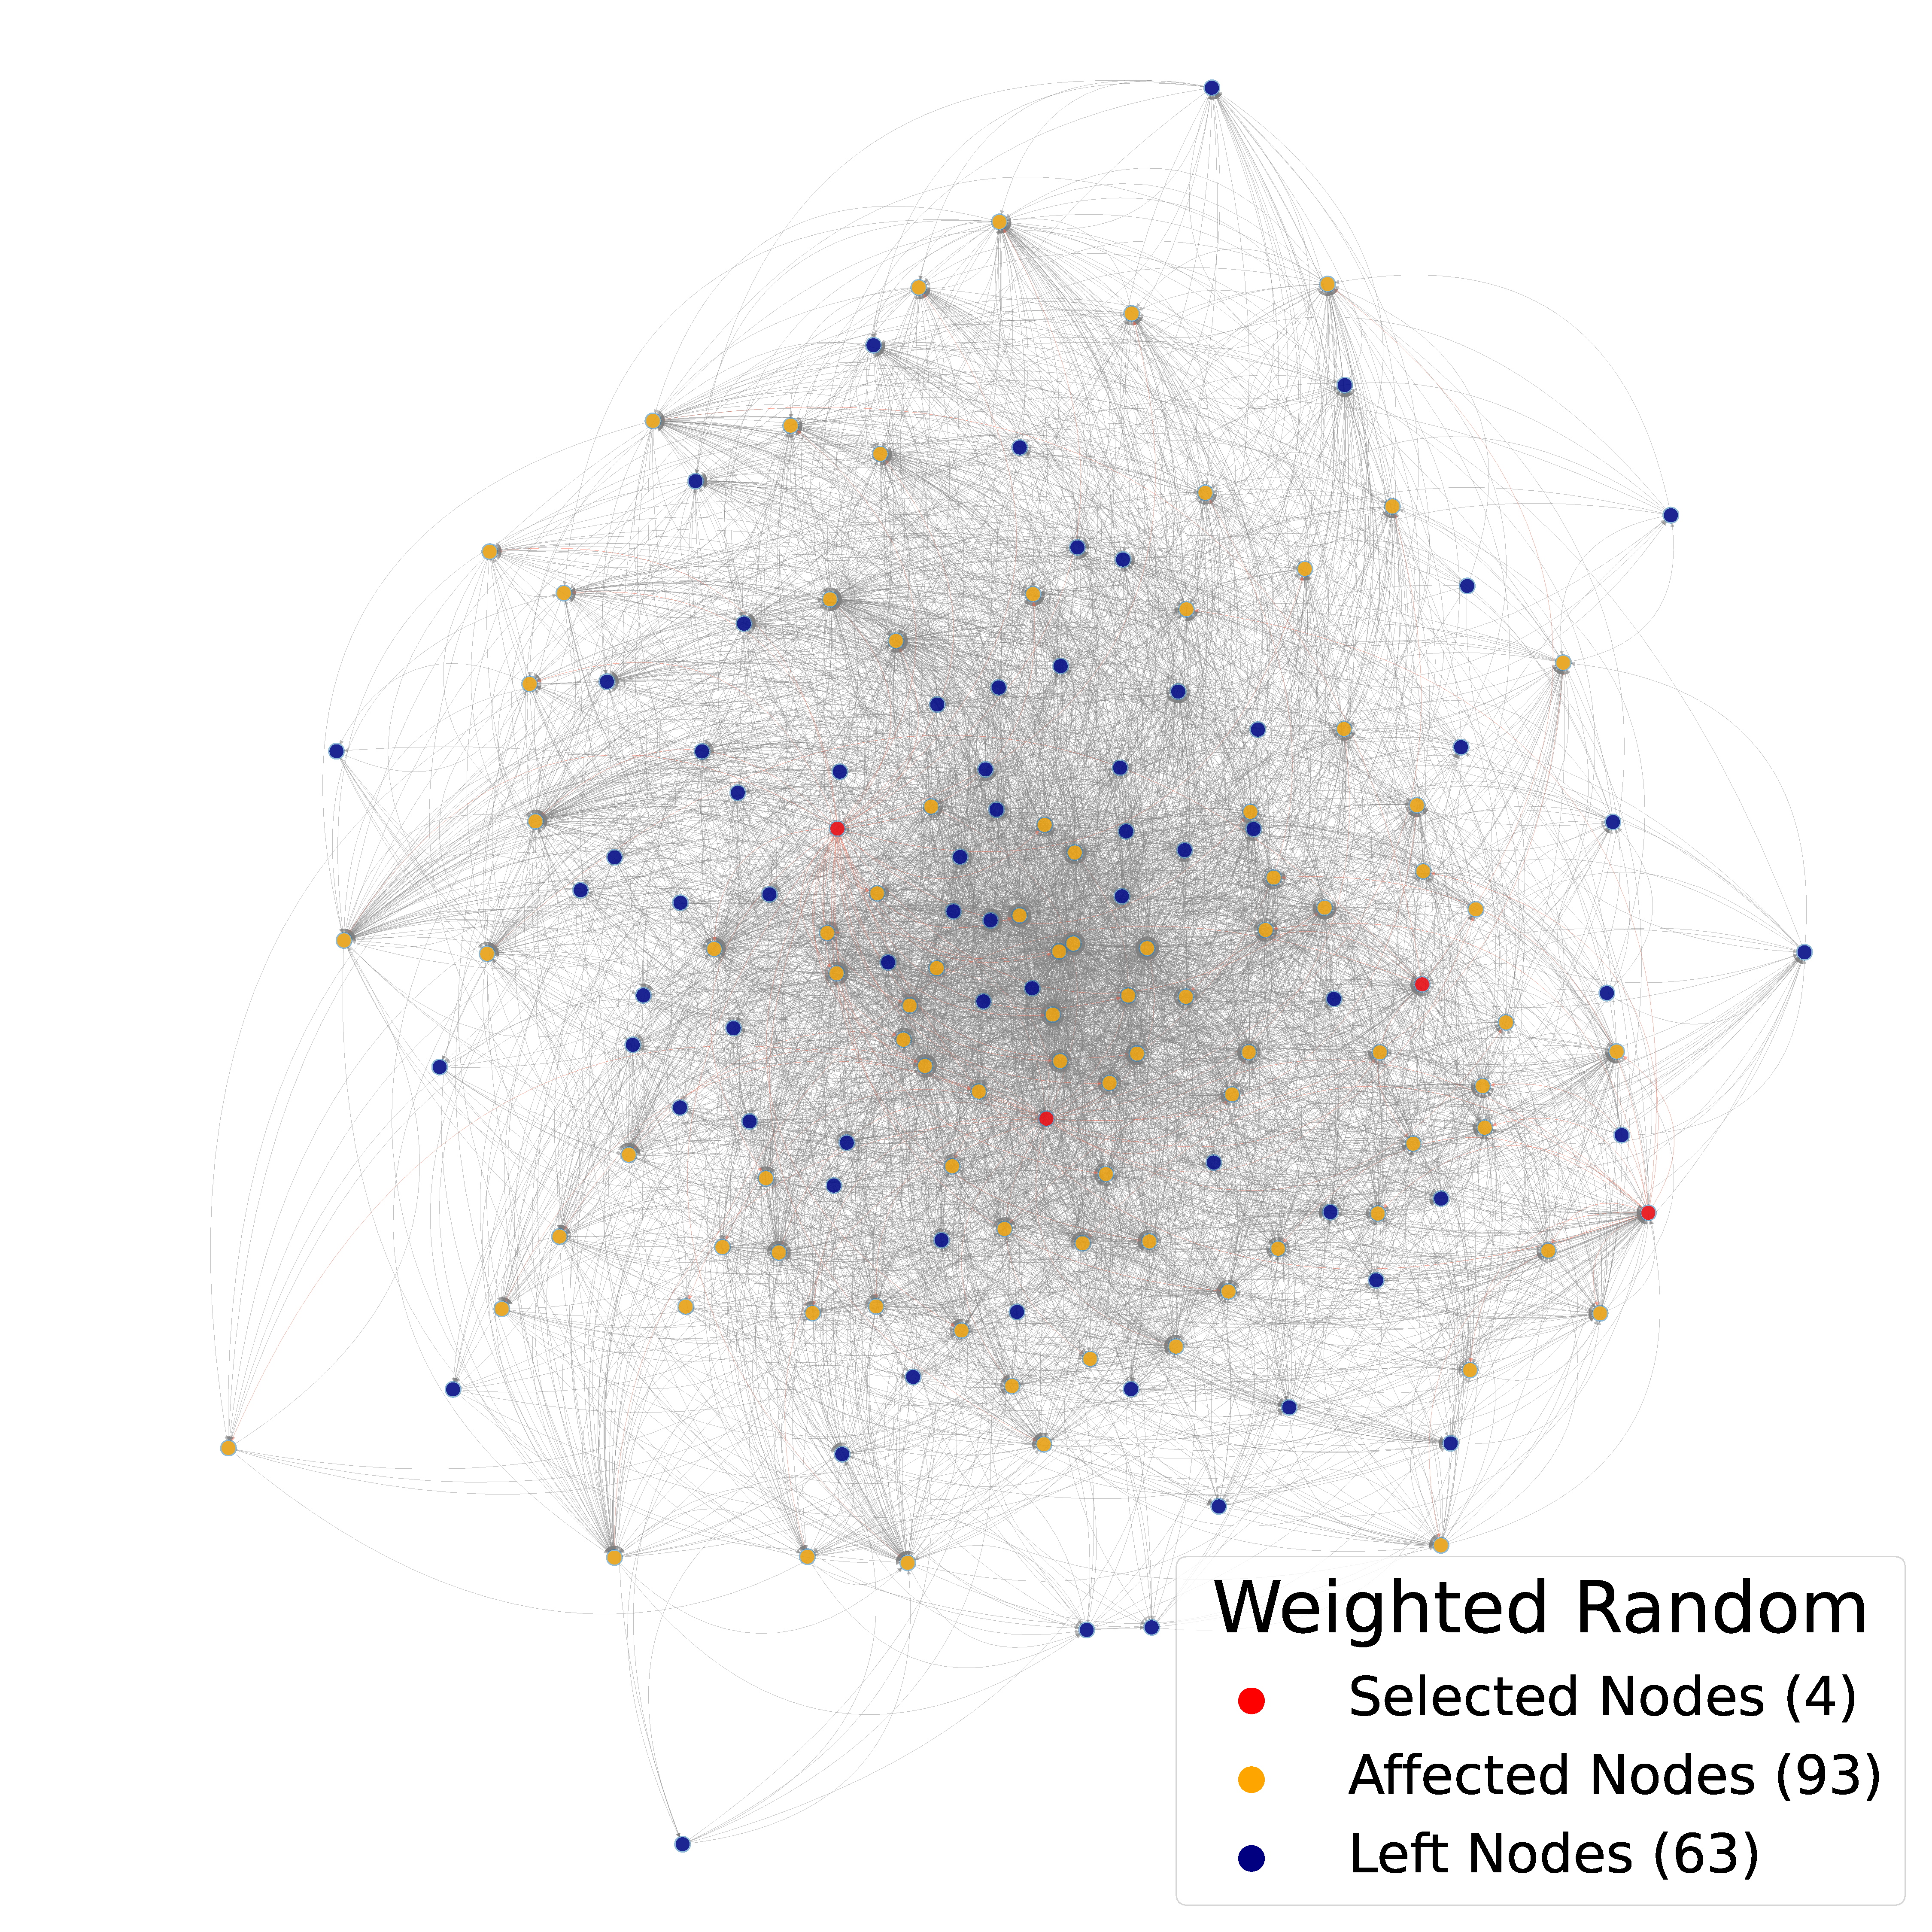
\includegraphics[width=\linewidth]{Figures/GraphExperiment/Network/plot_Weighted Random.pdf}
        %\\{\tiny Weighted Random}
        \label{fig:wr}
    \end{minipage}%\hspace{0.005\textwidth}
    \hfill
        % Fourth figure
    \begin{minipage}{0.18\textwidth}
        \centering
        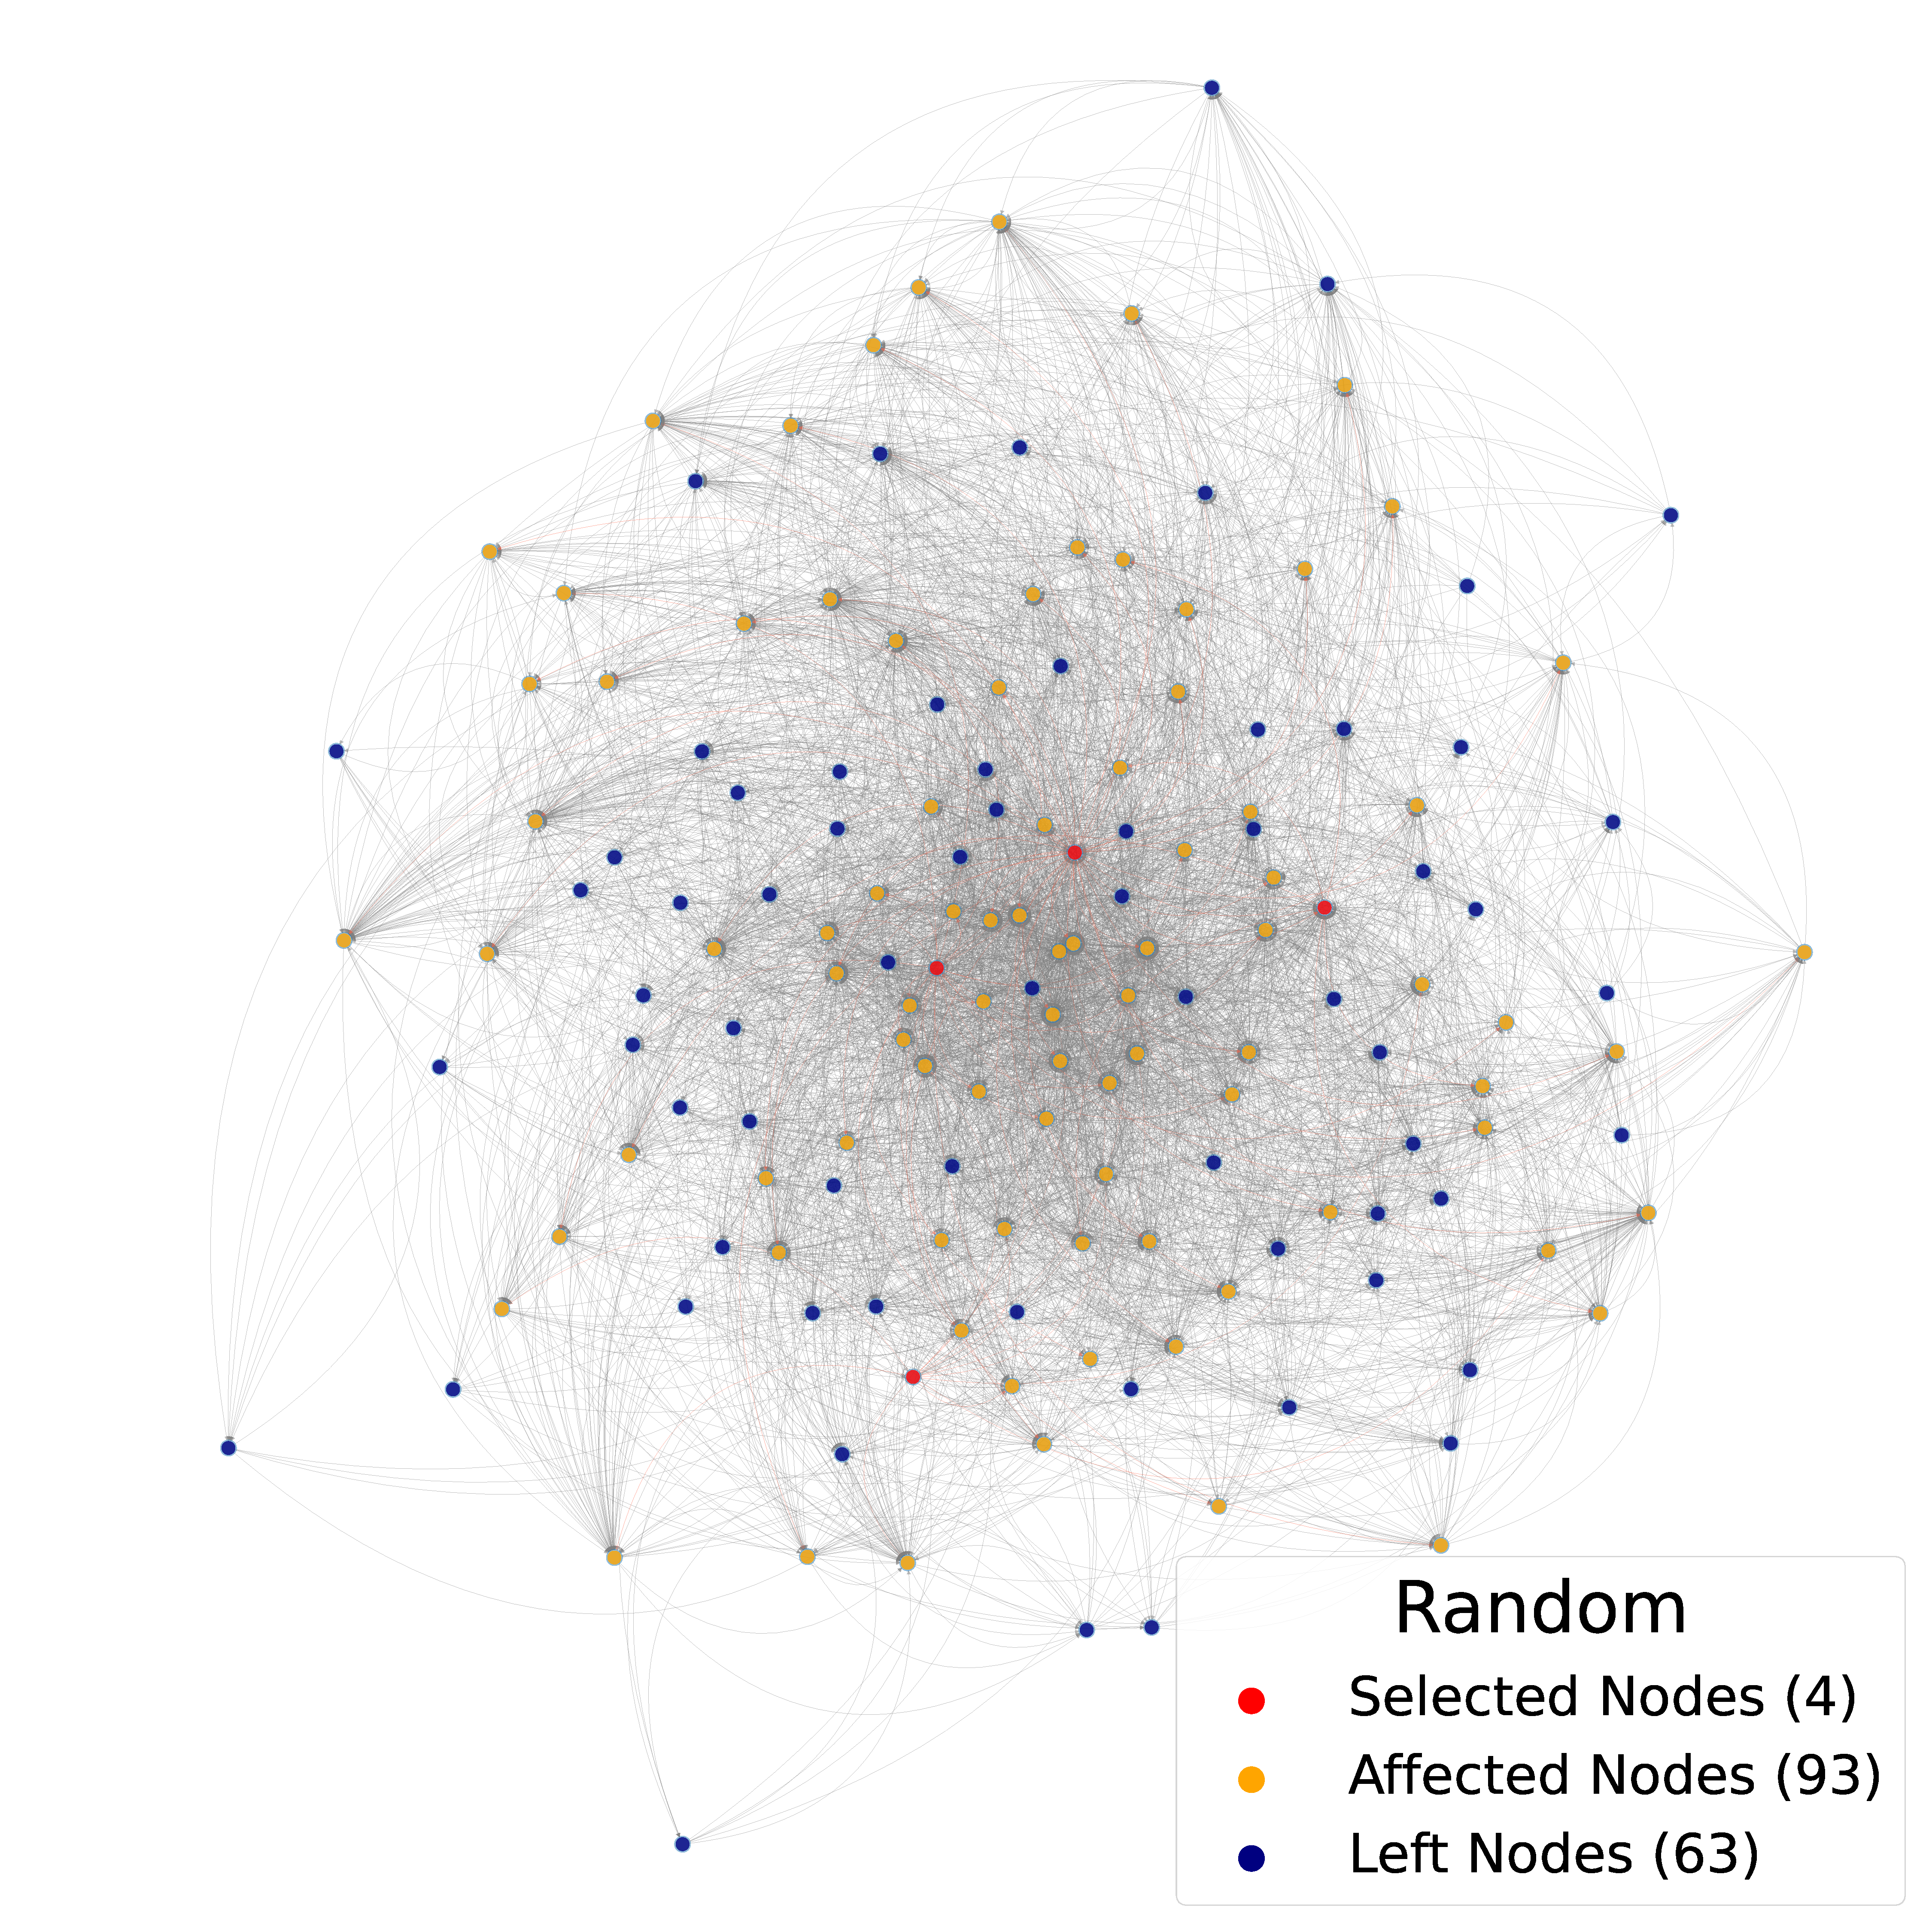
\includegraphics[width=\linewidth]{Figures/GraphExperiment/Network/plot_Random.pdf}
        %\\{\tiny Random}
        \label{fig:random}
    \end{minipage}%\hspace{0.005\textwidth}
    \hfill

    \caption{Node selection on a sub-network of Reddit ($K = 4$ and $\eta=4$). High-degree nodes are displayed in large sizes; selected nodes are marked red with red out-edges linked to affected nodes (orange). The performance decline from left to right.}
    \label{fig:network visualisation}
\end{figure*}


\begin{figure*}[t!]
    \centering
    % First figure
    \begin{minipage}{0.245\textwidth}
        \centering
        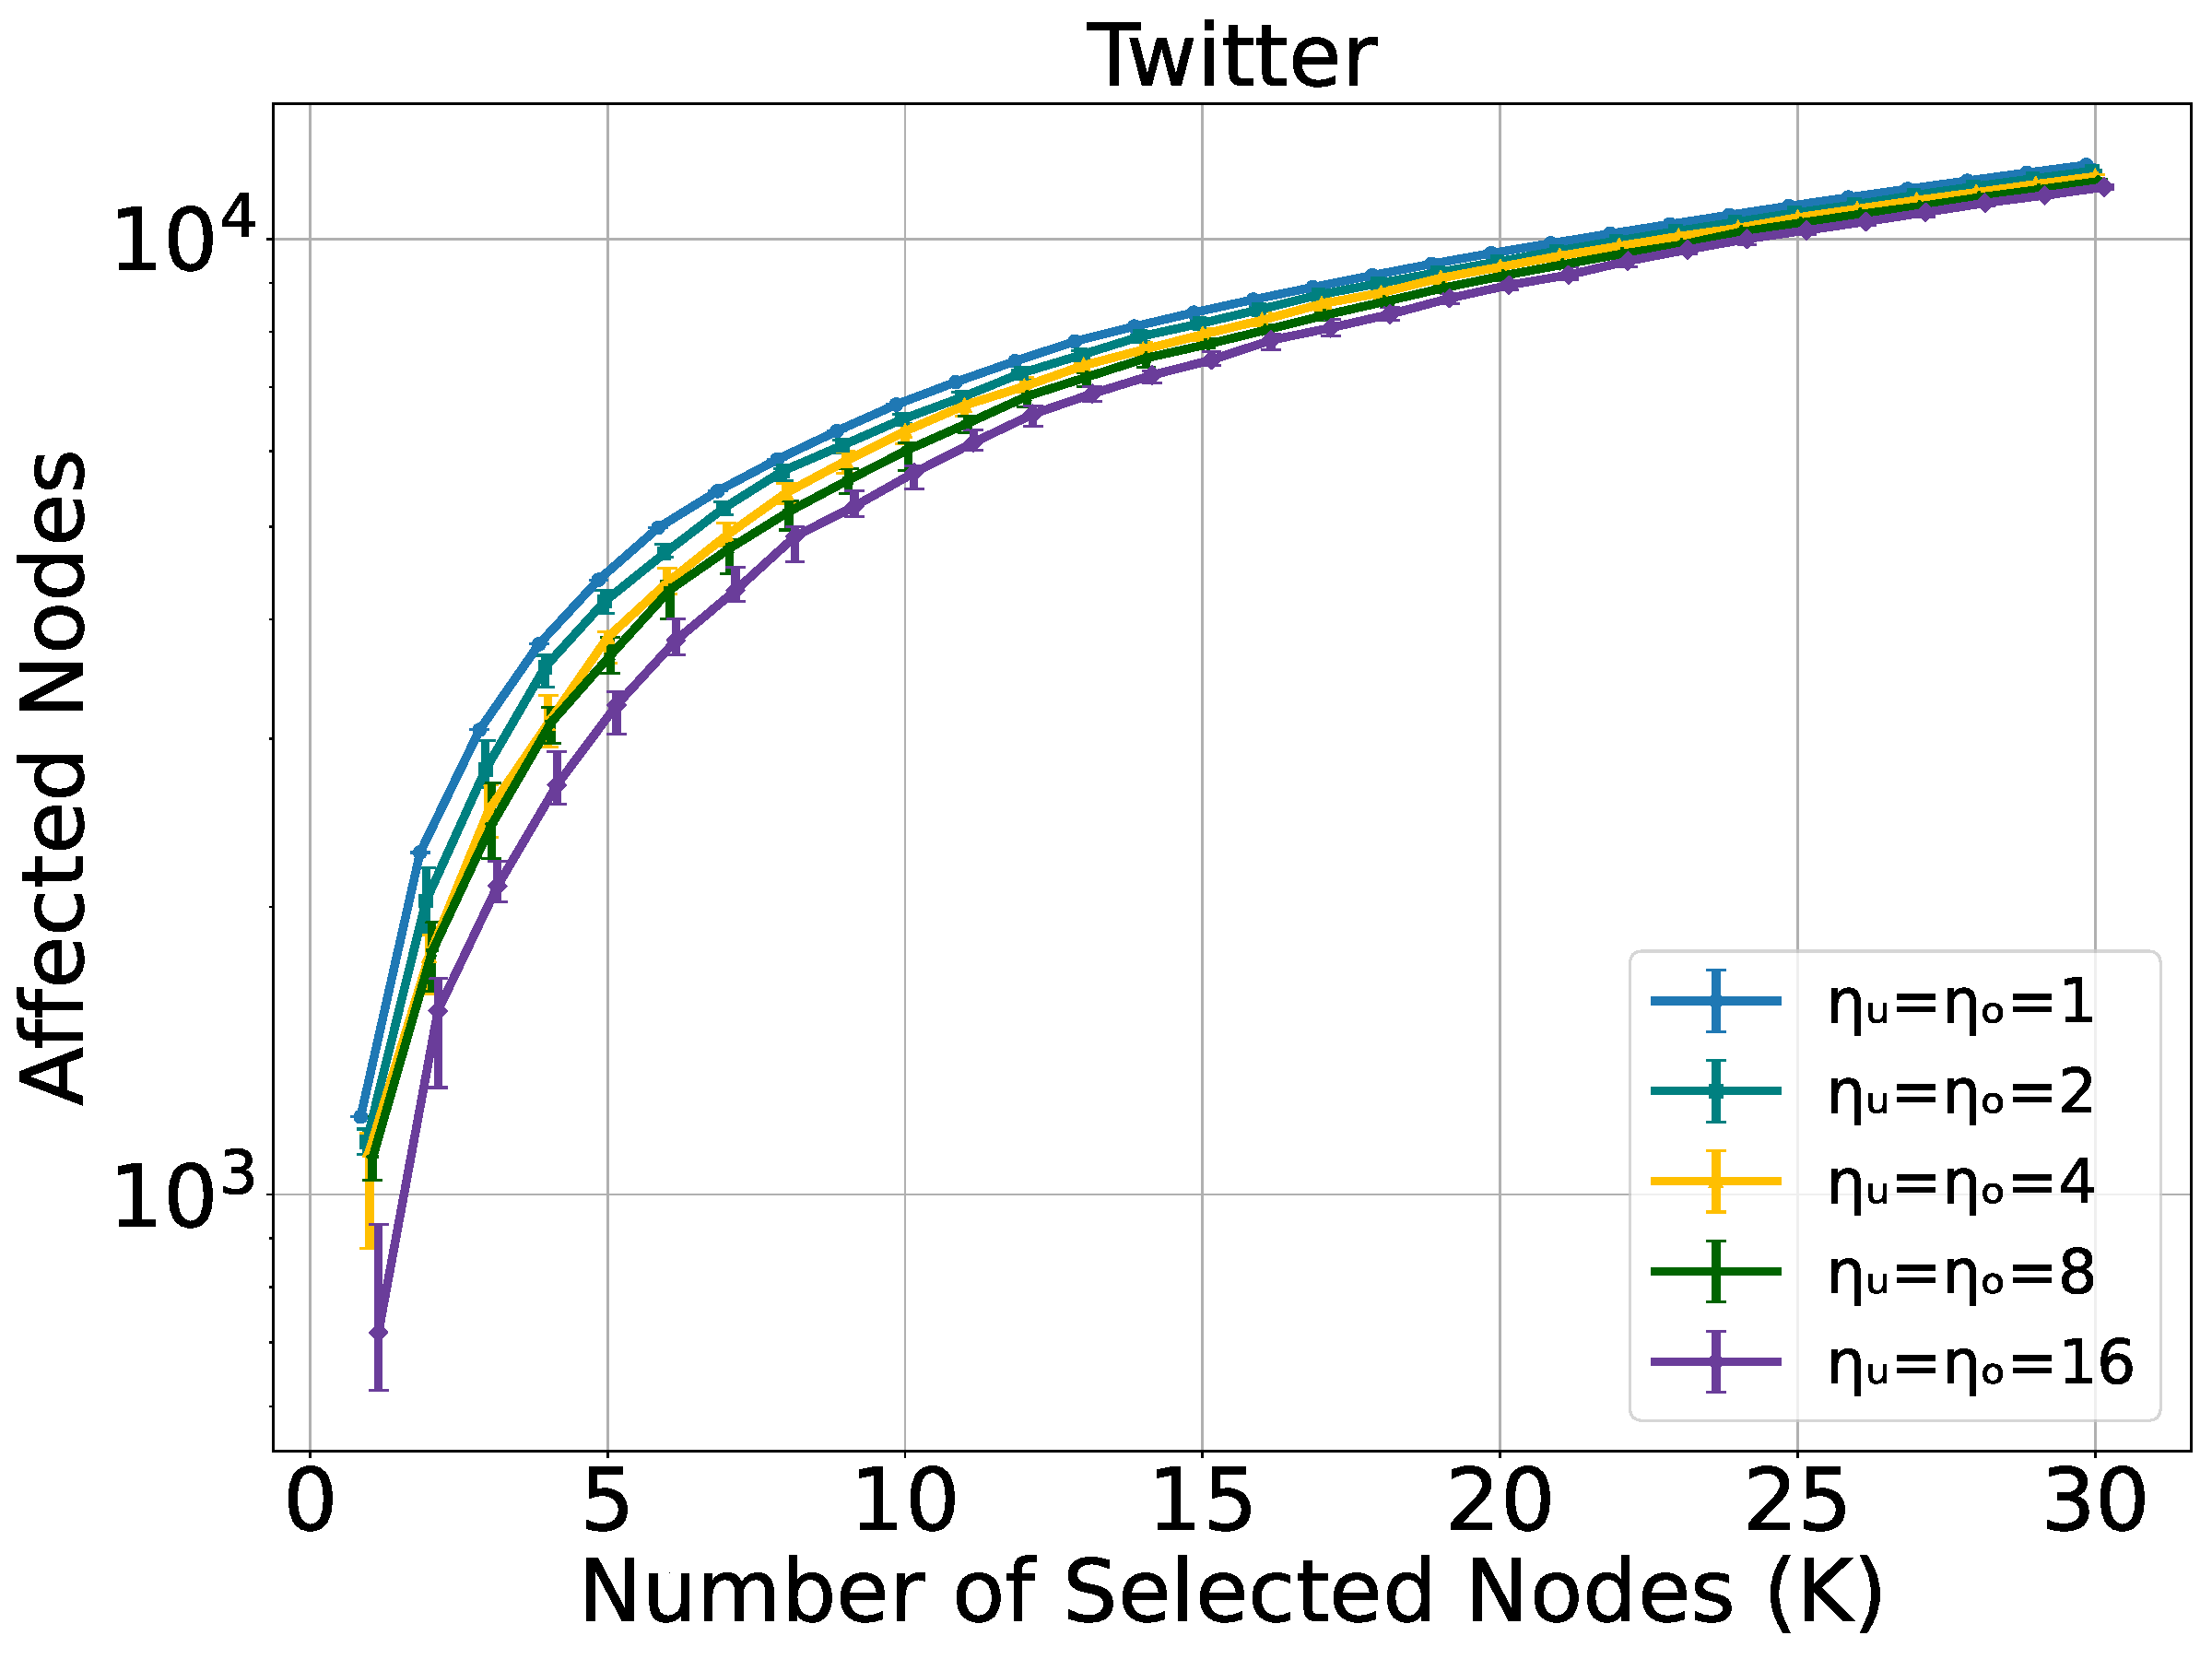
\includegraphics[width=\linewidth]{Figures/GraphExperiment/Errors/new/error_twt.pdf}
        \label{fig:error_twt}
    \end{minipage}\hfill
    % Second figure
    \begin{minipage}{0.245\textwidth}
        \centering
        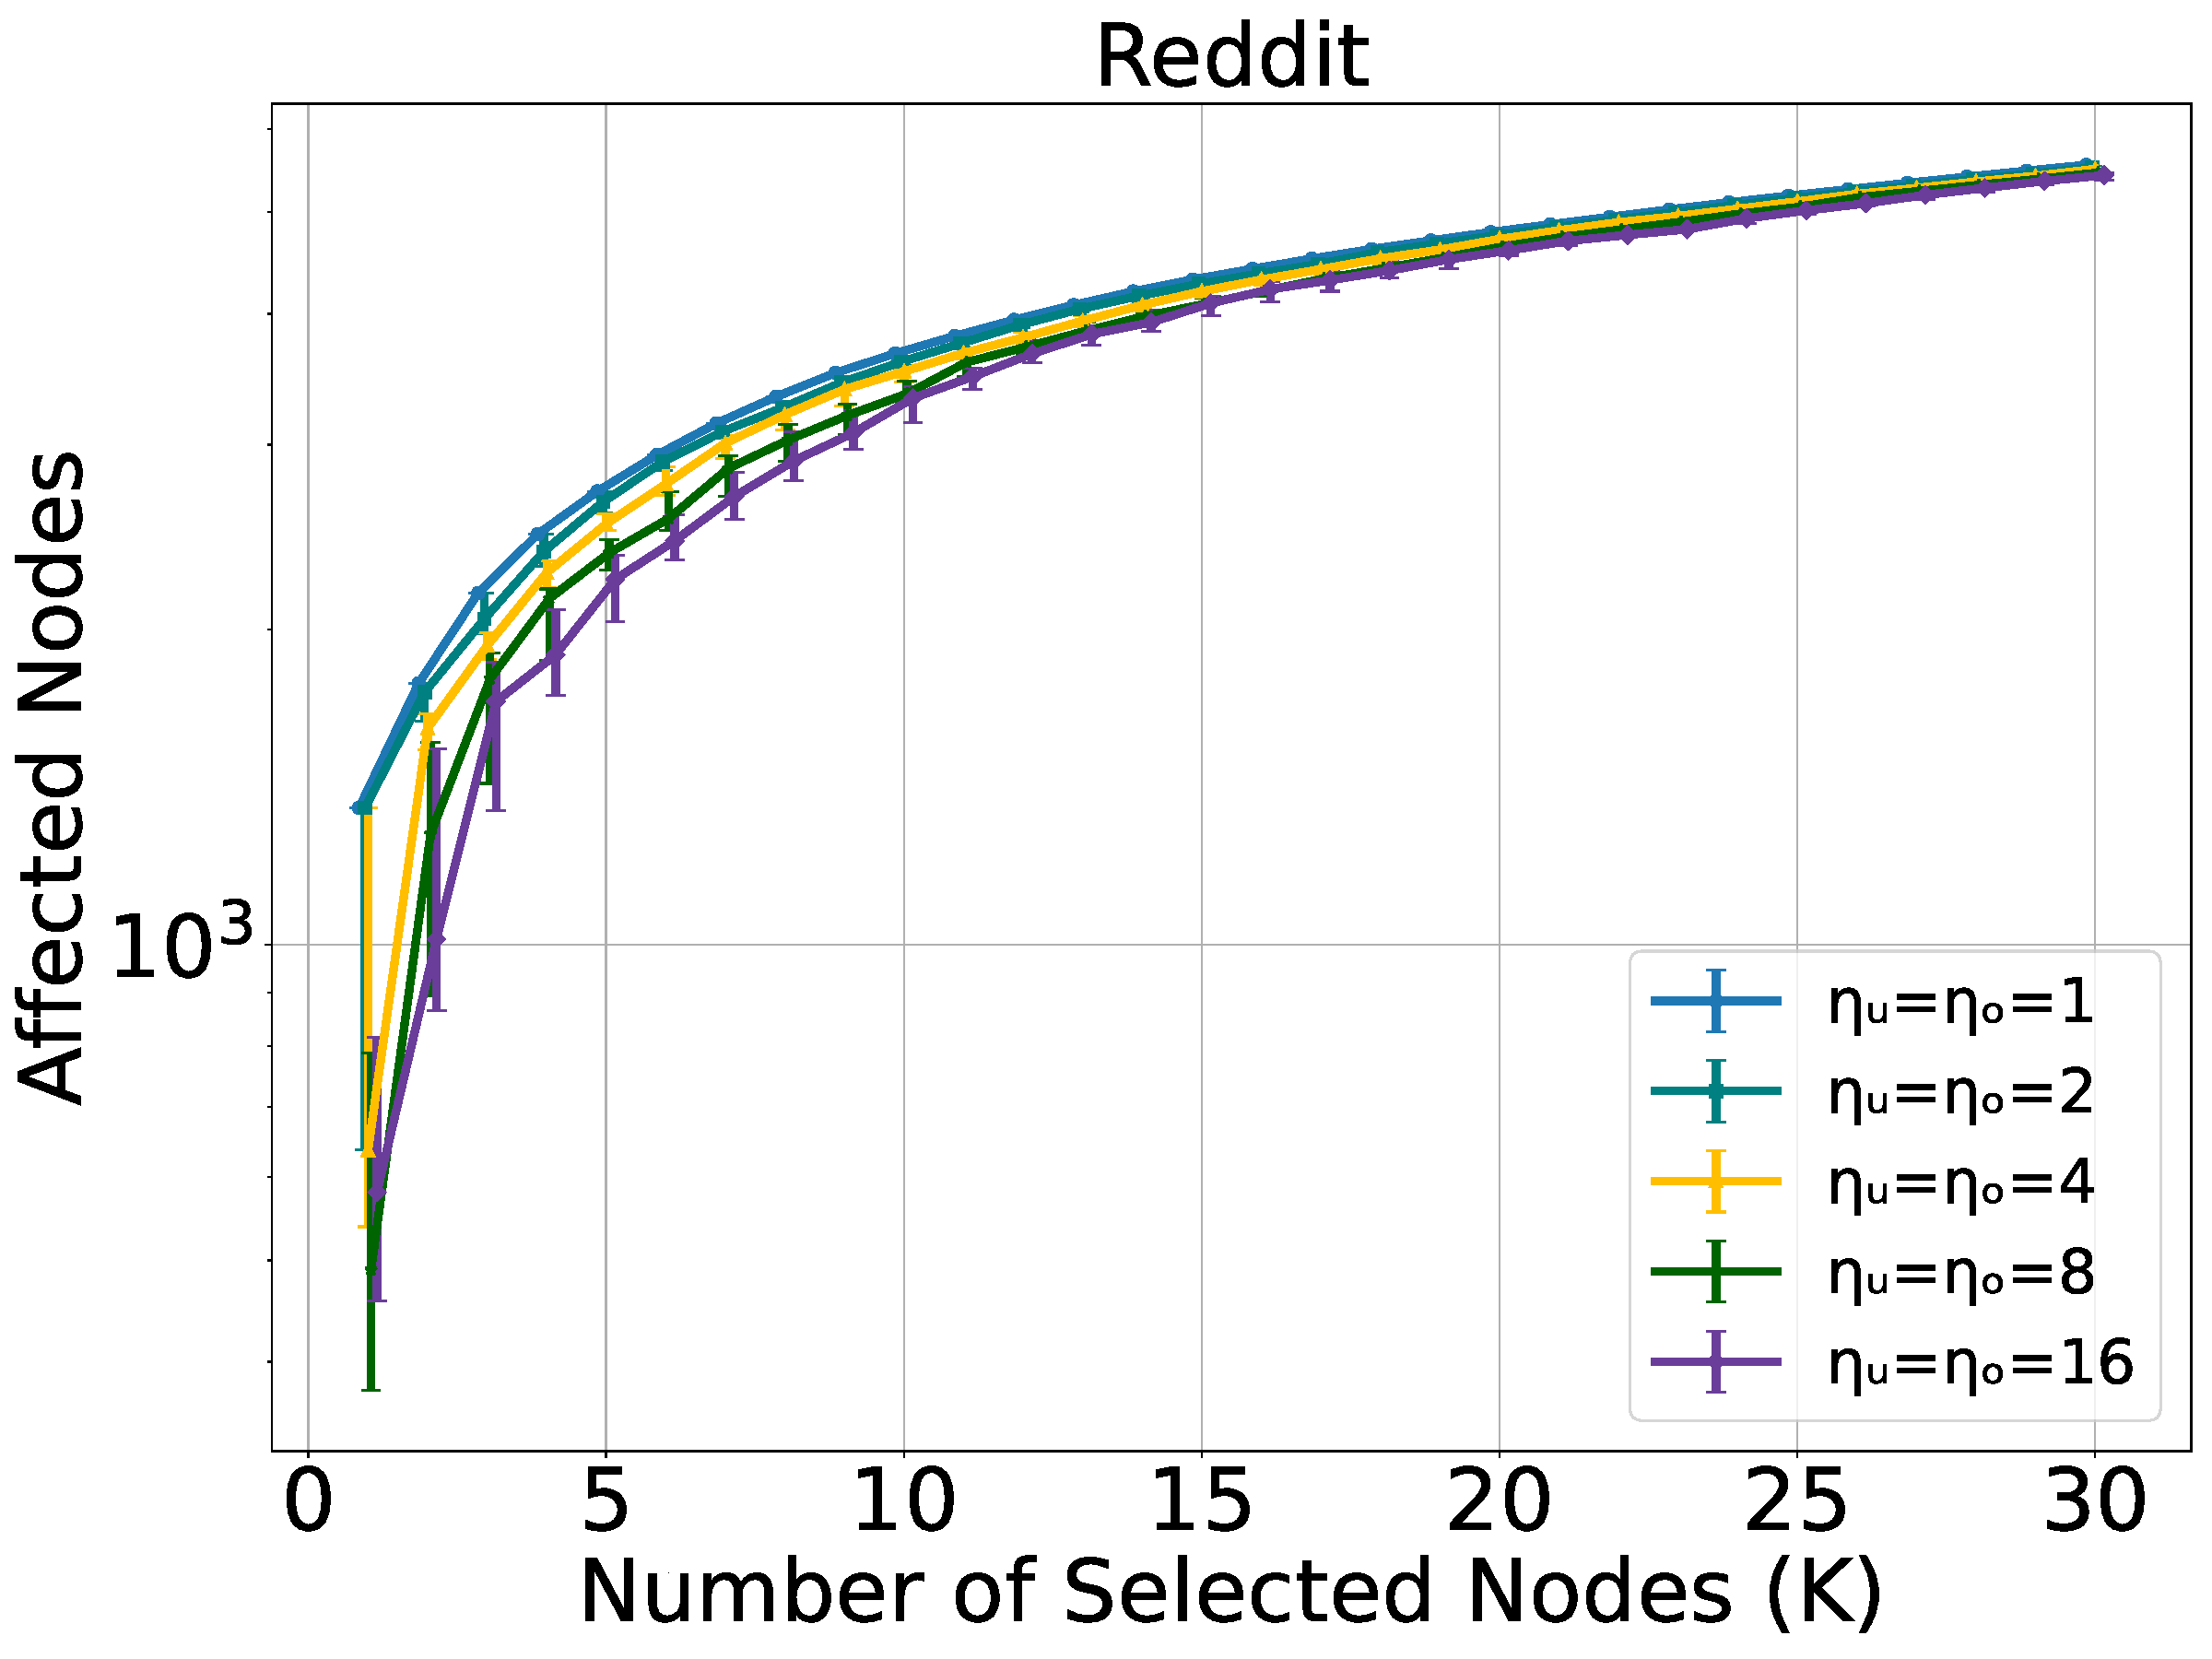
\includegraphics[width=\linewidth]{Figures/GraphExperiment/Errors/new/error_rdt.pdf}
        \label{fig:error_rdt}
    \end{minipage}
    \hfill
    % Third figure
    \begin{minipage}{0.245\textwidth}
        \centering
        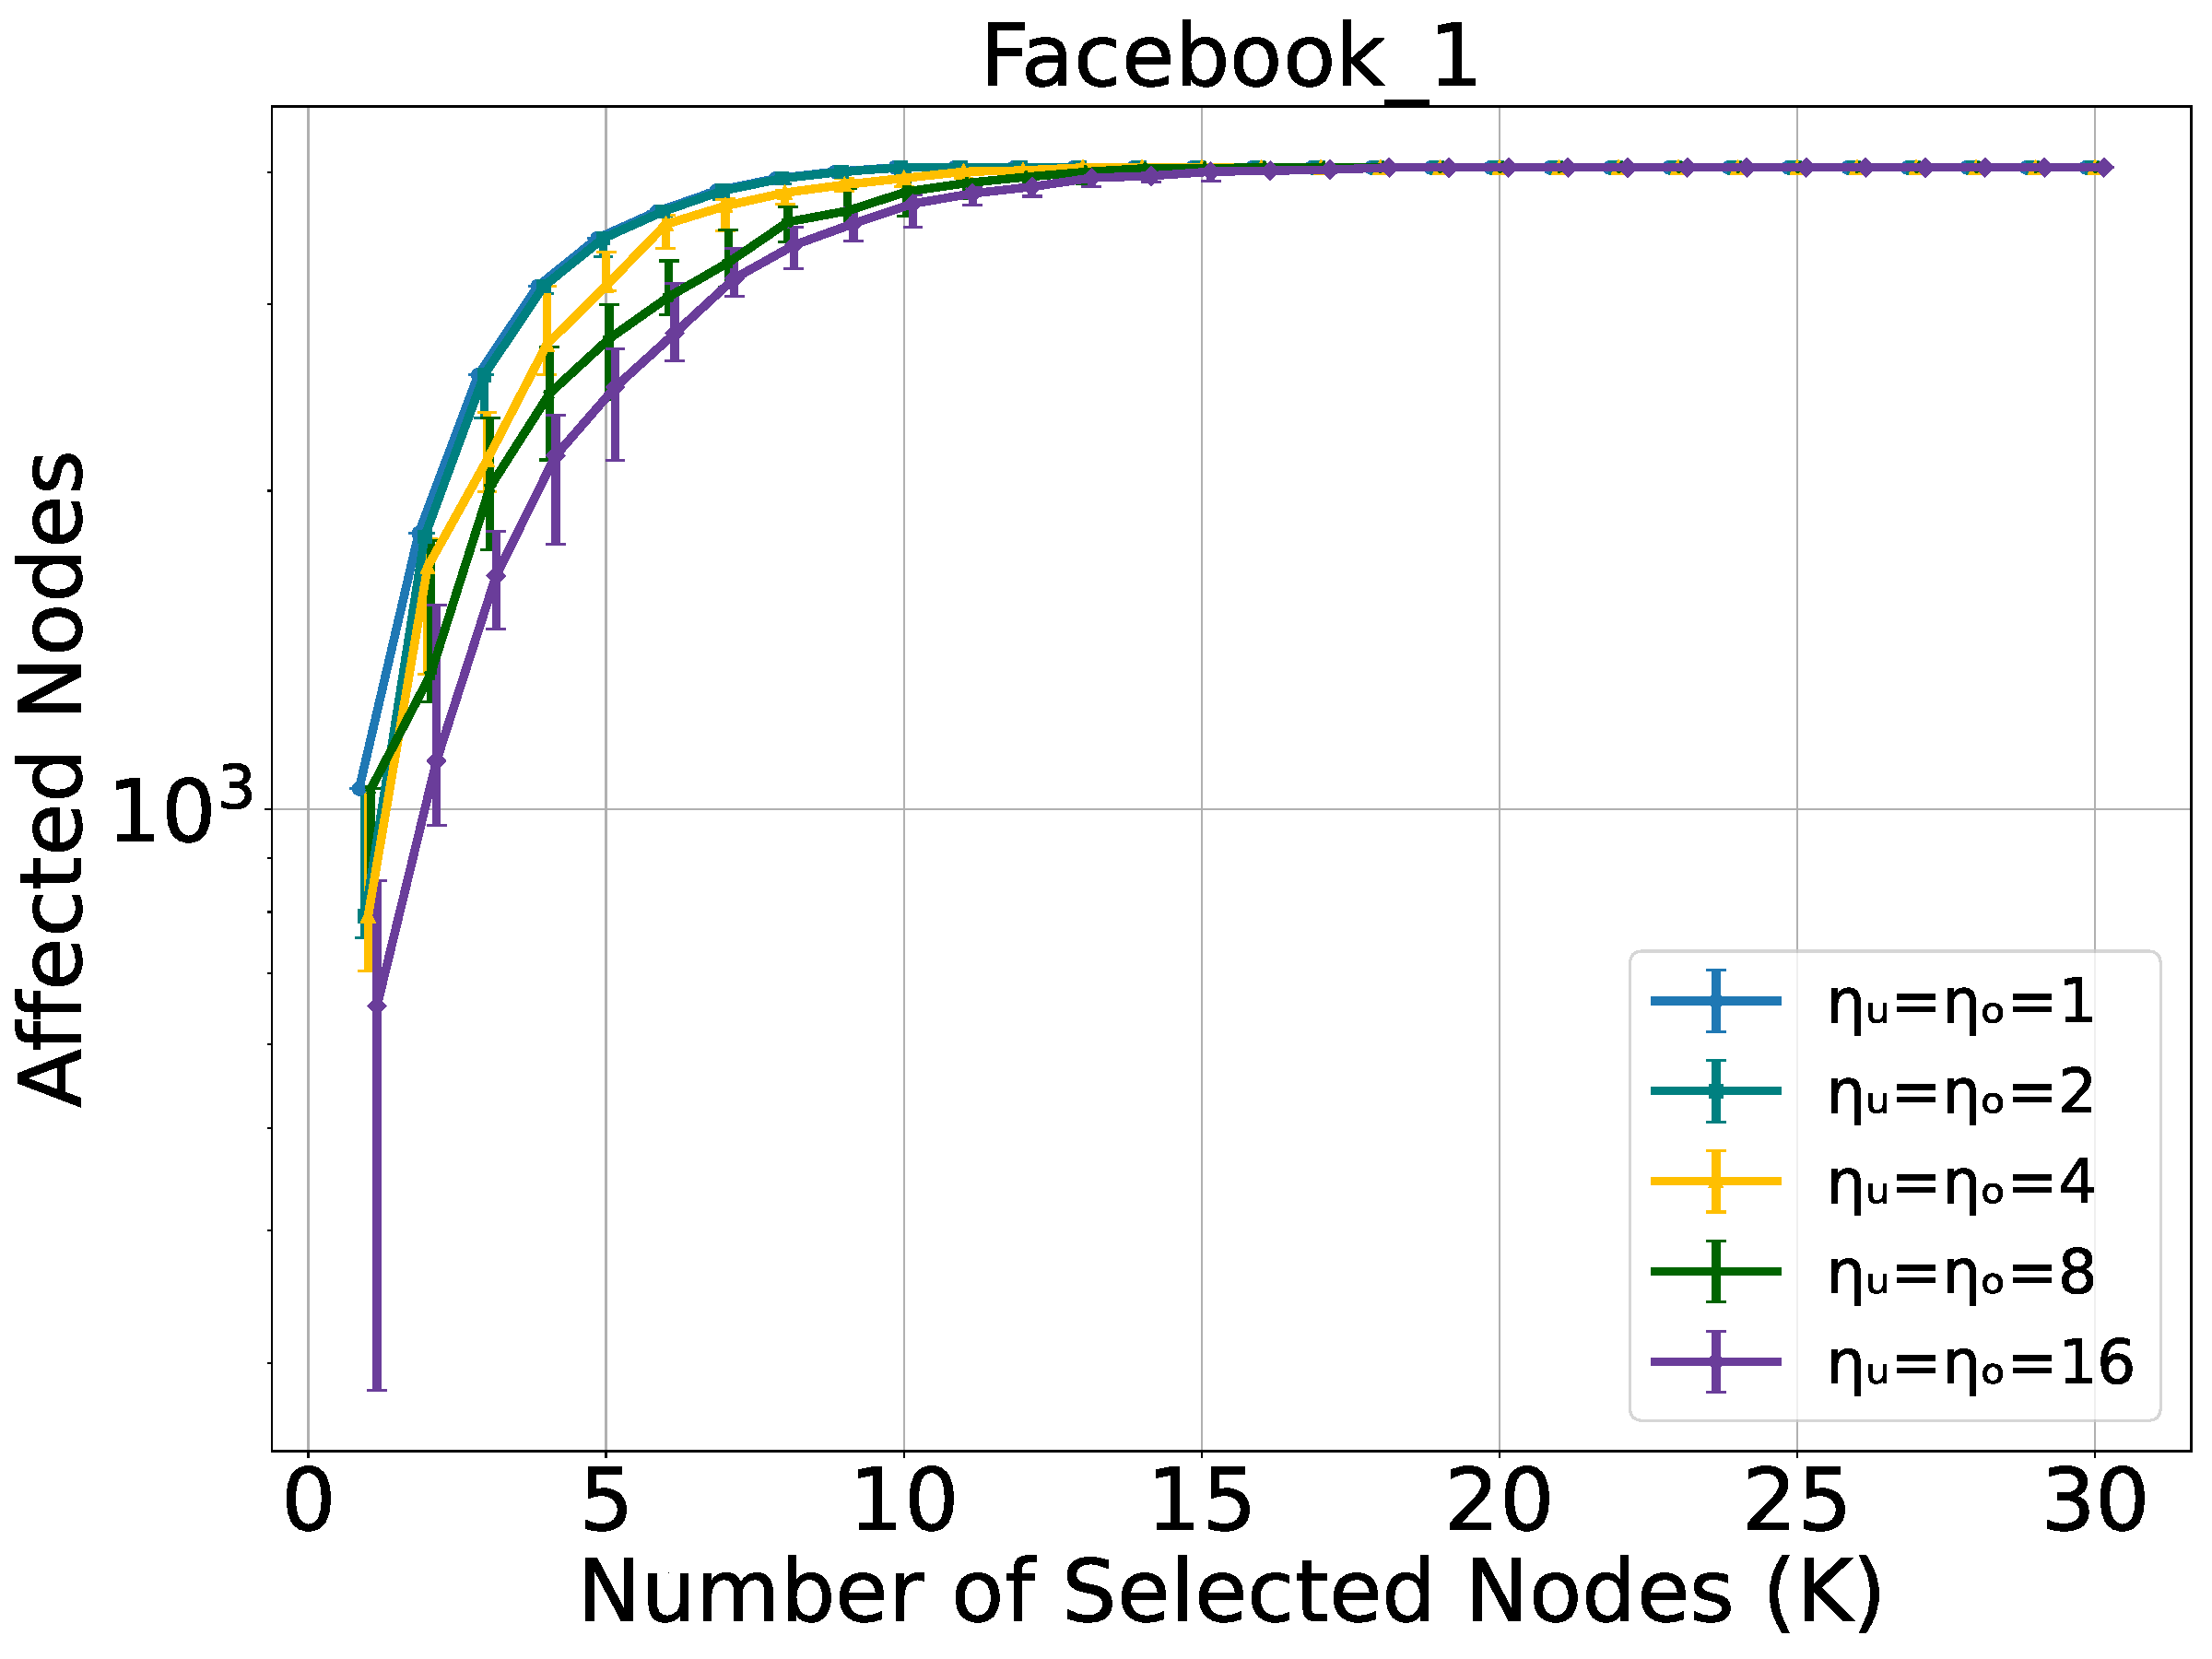
\includegraphics[width=\linewidth]{Figures/GraphExperiment/Errors/new/error_fb1.pdf}
        \label{fig:error_fb1}
    \end{minipage}
    \hfill
    % Fourth figure
    \begin{minipage}{0.245\textwidth}
        \centering
        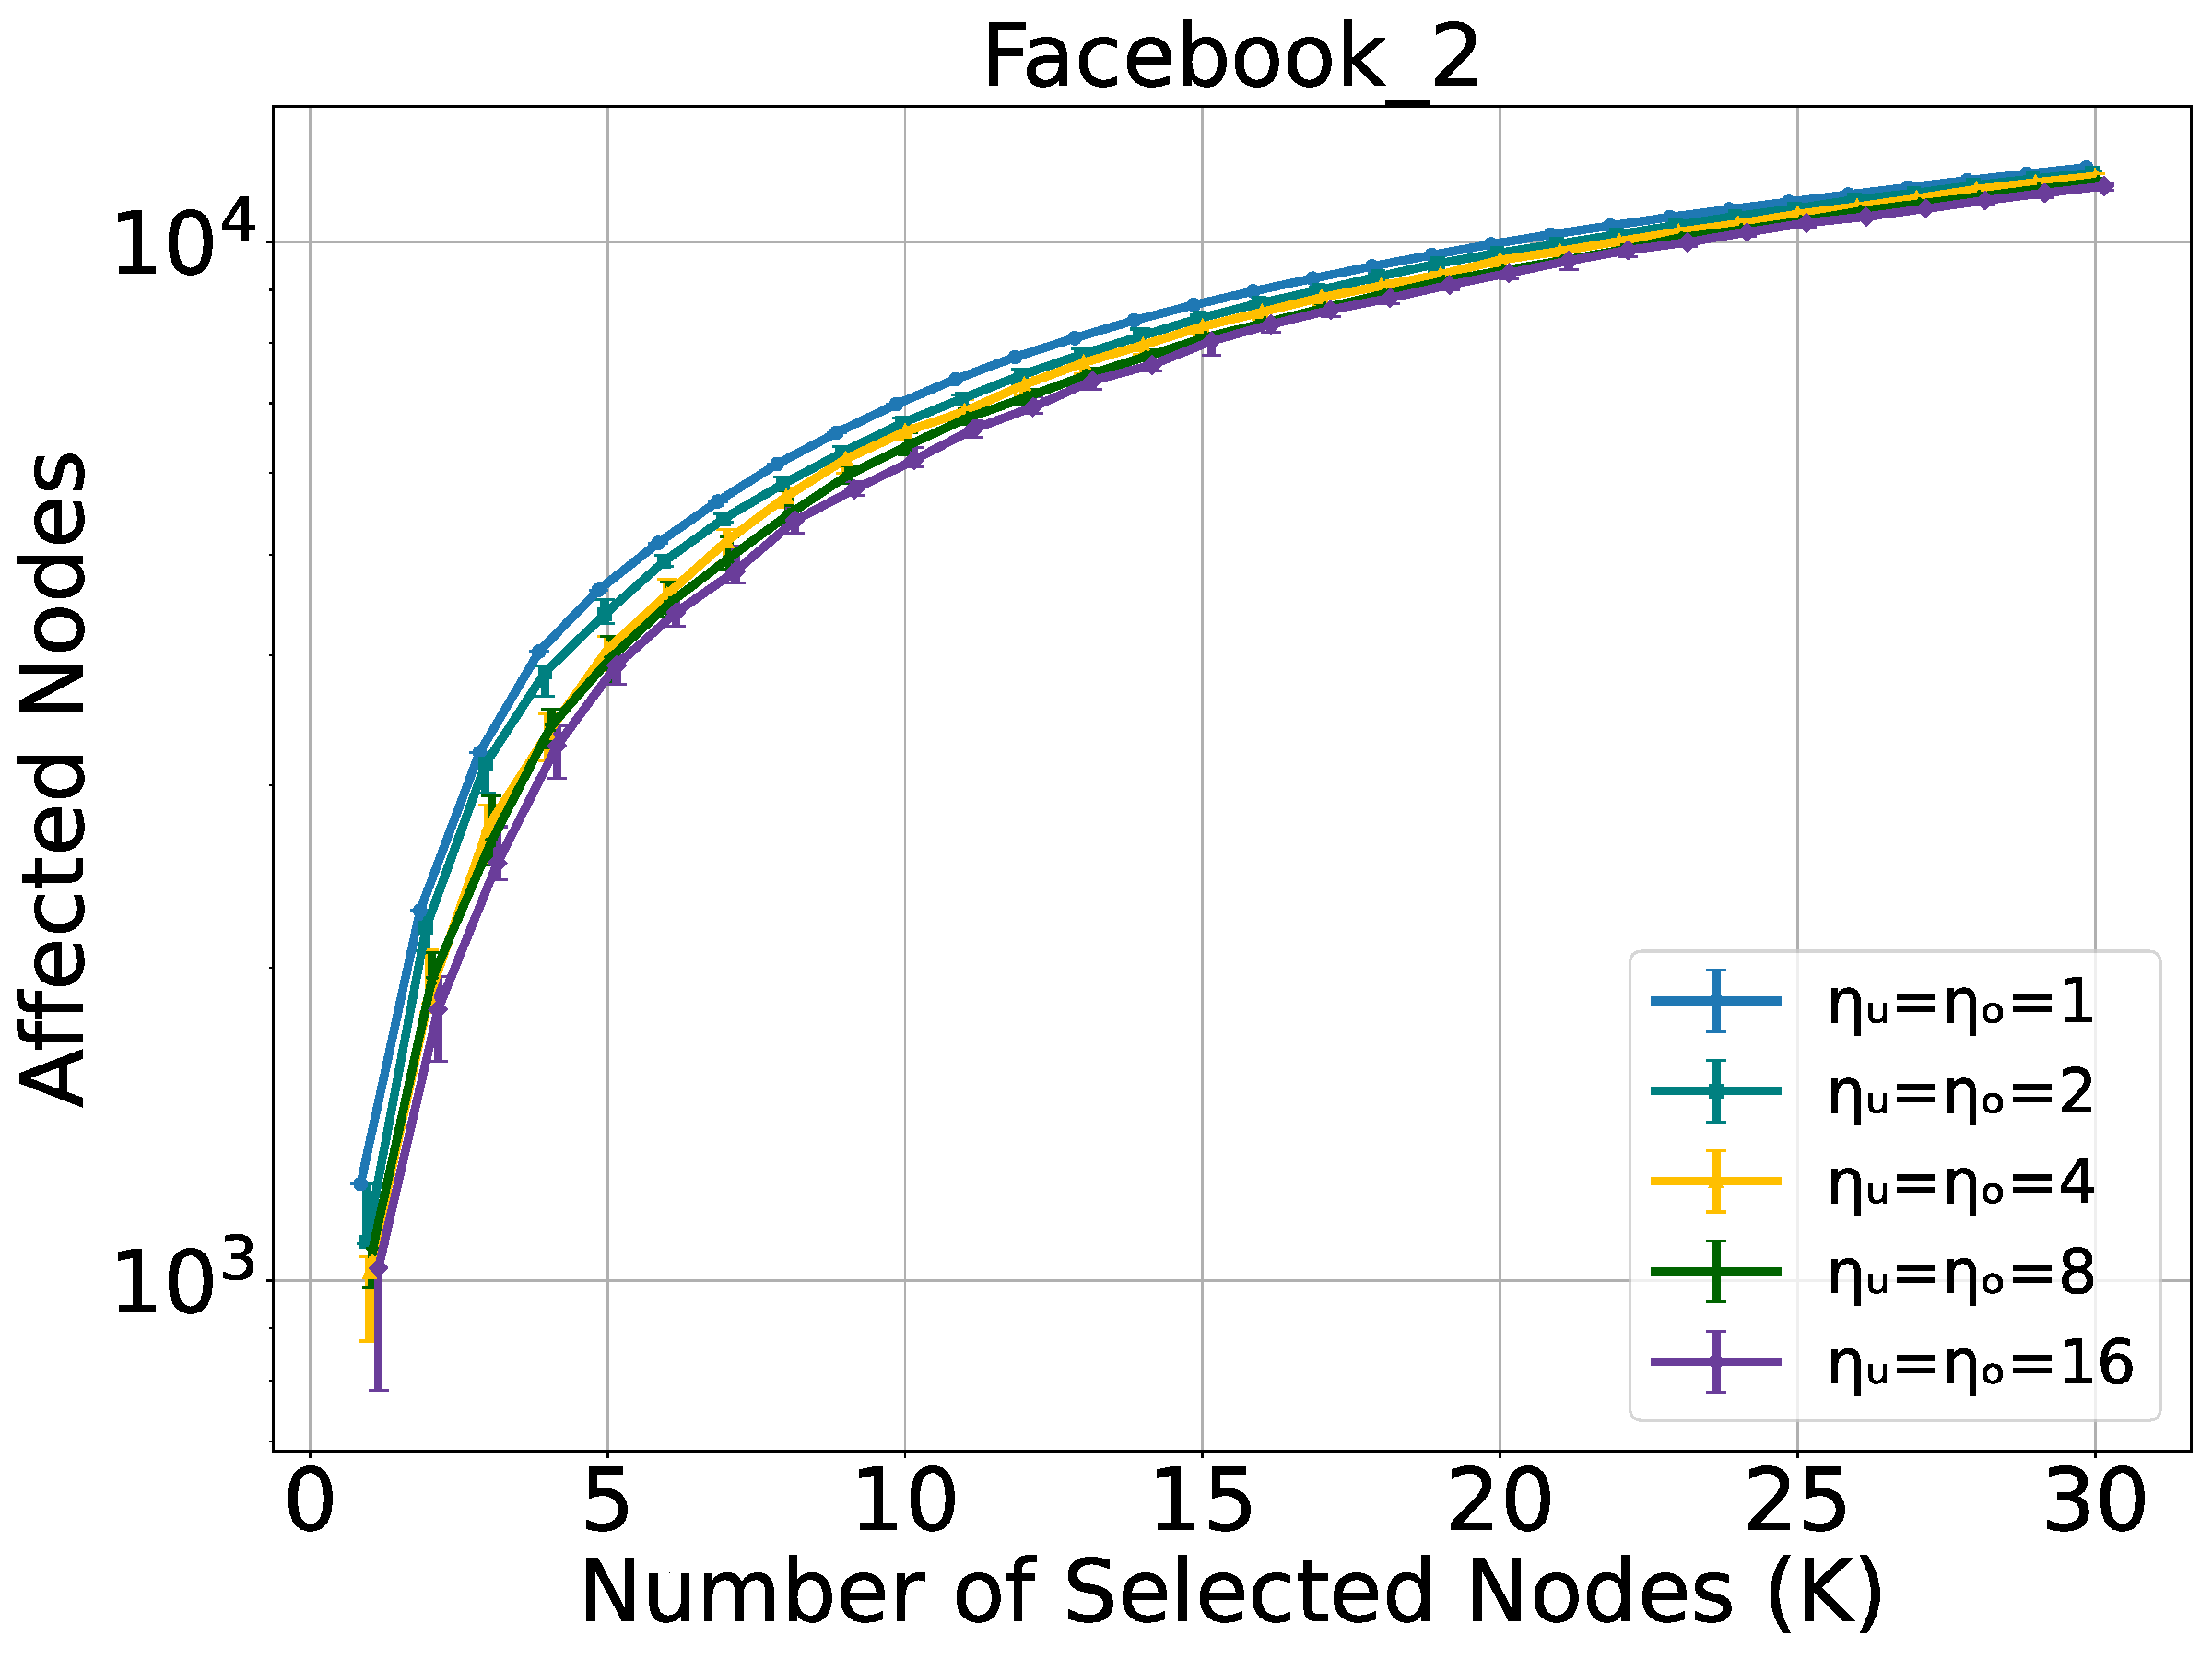
\includegraphics[width=\linewidth]{Figures/GraphExperiment/Errors/new/error_fb2.pdf}
        \label{fig:error_fb2}
    \end{minipage}
    %\vspace*{-5mm}
    
    \caption{Affected nodes with an increasing $K$ by SOP-Greedy with $\eta \in [1, 16]$.}
    \label{fig:graph error}
\end{figure*}

\begin{figure*}[t!]
    \centering
    % First figure
    \begin{minipage}{0.245\textwidth}
        \centering
        
\includegraphics[width=\linewidth]{Figures/experiment 2/new/c2_twt.pdf}
        \label{fig:RSOP_C_twt}
    \end{minipage}\hfill
    % Second figure
    \begin{minipage}{0.245\textwidth}
        \centering
        
\includegraphics[width=\linewidth]{Figures/experiment 2/new/c2_rdt.pdf}
        \label{fig:RSOP_C_rdt}
    \end{minipage}
    \hfill
    % Third figure
    \begin{minipage}{0.245\textwidth}
        \centering
        
\includegraphics[width=\linewidth]{Figures/experiment 2/new/c2_fb1.pdf}
        \label{fig:RSOP_C_fb1}
    \end{minipage}
    \hfill
    % Fourth figure
    \begin{minipage}{0.245\textwidth}
        \centering
        
\includegraphics[width=\linewidth]{Figures/experiment 2/new/c2_fb2.pdf}
        \label{fig:RSOP_C_fb2}
    \end{minipage}

    \caption{Comparisons of SOP-Greedy and RSOP-Greedy with increasing $K$ under various $\eta_u$ and $\eta_o$.
    %\ref{appendix:large-scale}.
    }
    \label{fig:RSOP_C}
\end{figure*}



\textbf{Experimental set-up.} We consider two classification tasks: airline passenger satisfaction classification \cite{jiang2022forecast} and breast cancer detection \cite{assegie2021breast}. The benchmarks are \textit{SelectKBest} \cite{otchere2022application}, \textit{Recursive Feature Elimination (RFE)} \cite{sachdeva2022systematic}, \textit{Mutual Information} \cite{feature-selection}, and \textit{Extra Trees} \cite{extra-trees}. %Descriptions of data and benchmarks are in Appendix D. %\ref{appendix:descriptions-data-benchmarks}. 
Both tasks have the following set-up. 
Data are randomly split into training data (80\%) and oos data (20\%). The model $h$ is decision tree with the default hyper-parameters and fitting procedure of \textit{scikit-learn}. 
Function $\mathcal{L}$ is the oos accuracy. 
The cardinality constraint $K$ varies from $1$ to $7$. 
%, due to the initial observation that further increasing $K$ does not change accuracy. 
The predictor $\tilde{f}$ is an \textit{independent erroneous oracle}: querying $d_B(A)$ returns $d_B(A) \cdot \text{exp}(X)$ with $X \sim \mathcal{U}(-\log \eta_u, \log \eta_o)$, where $\eta = \eta_u \cdot \eta_o \in [1, 400]$. We know that sampling can exploit independent errors to achieve vanishing errors \cite{submodularOptNoisetoImageCollection}. However, in our implementation, value $d_B(A)$ is queried at most once for any $A, B \subseteq [n]$, making errors effectively \textit{consistent}. 
We implement the R-step predictive greedy ($R = 1, 2, 3$), which we call SOP-Greedy (Submodular Optimization Predictive Greedy). %, with implementation details. %\ref{appendix:experiment1-implementations} 
We run the predictive greedy 30 times and report InterQuartile Range (IQR) of the results to take the randomized error generation into account. We also compute a lower bound for the empirical performance ratio of SOP-Greedy defined as $\frac{f(S_{\text{SOP}})}{\mathrm{OPT}}$, where $S_{\text{SOP}}$ denotes the solution returned by SOP-Greedy and OPT the optimal value. We set $\text{OPT} = 1$ to under-estimate the true ratios. The experiments are conducted with processor Intel Core 12600KF, RAM 16GB, and GPU Nvidia Geforce RTX 3070, 8GB VRAM. 

% Present the results; discuss observtions and implications

\textbf{Results.} Figure \ref{fig:experiment1-performance} presents the oos accuracy for different algorithms on two datasets with varying $K$ and $\eta$. The accuracy under an increasing $K$ is approximately increasing and concave, reflecting diminishing gains. 
%\textcolor{red}{it shows the consistency between the submodular function and SOP-Greedy.} 
SOP-Greedy can access $\tilde{f}$, but the other benchmarks can use $\boldsymbol{X}$ and $y$ to measure in-sample correlations between features and targets. The results show that SOP-Greedy consistently outperforms the benchmarks for $K > 1$. One may argue that the superiority may be attributed to the informational advantage of knowing the (erroneous) oos performance. However, the algorithm maintains robust performance even with unreasonably large errors (up to $400$), i.e., the errors merely affect performance. This suggests that predicting the exact oos performance might be less critical than the ordering of the oos performance for different feature sets. It shows that (1) the OOS performance forecasts are solid indicators for feature selection, even if they might be far from accurate, and (2) robustness of SOP-Greedy under bad predictions. The performance downgrades gracefully with increasing prediction errors, as shown in the last two figures, showing the smoothness of SOP-Greedy. 
%showcasing its substantial robustness by remaining successful even under worst-case prediction errors. 
%The smoothness is validated by changing the error values because the algorithm's performance is consistent across different prediction qualities.


Figure \ref{fig:experiment2-R-step} presents the oos accuracy of the R-step predictive greedy (RSOP-Greedy) with varying $R$. The algorithm observes slight improvements with an increased $R$. Still, the improvements are insignificant, although the theoretical worst-case bounds are improved. We suspect this might be because the errors are not adversarial, so the benefit of searching a larger space is marginal. The estimated empirical performance ratios of SOP-Greedy against the theoretical bounds are shown in Tables \ref{tab:airline-r-steps-theo} and \ref{tab:breast-r-steps-theo}. The empirical performance ratios well-exceed the theoretical bounds derived previously. This suggests that our theoretical bounds are pessimistic even if we assume OPT is 1, showing that the algorithm performs comparably to the optimum in practice. 






%The results constantly demonstrate that this methodology outperforms the results of the four benchmark methodologies: the approach's higher performance is primarily attributed to its dynamic gain computation, which is distinguished from the other four techniques. 

%It is noted that as the value of \( K \) grows to a certain threshold, the gains obtained by incorporating additional features start to reduce. After reaching this stage, the accuracy stabilizes and remains nearly constant. 

%The slowing down effect suggests that the predictive power of including additional features decreases once the model has already caught the most important features. This observation is aligned with the properties of submodular functions.

%Besides, our study investigates the impact of changing the error boundaries (\( \eta_u, \eta_o \)) on accuracy across different feature counts \( K \). When the error boundaries (\( \eta_u, \eta_o \)) are reduced, the precision of the feature subsets increases, which could be oberserved in Figure 1 (c) and (d). The above behavior is consistent with the expectation that a more accurate calculation of gains results in an improved selection of features and, therefore, superior performance of the model.






\subsection{Influence maximization} \label{subsec:influence-maximization}


The influence maximization problem models applications like a company targeting individuals in a social network to maximize their influence in a viral marketing campaign under some budget constraint \cite {kempe2003maximizing, bogunovic2017robust, banihashem2023dynamic}. Given a network $G = (V, E)$, our task is to find nodes $S \subseteq V, |S| \leq K$, with the maximum affected nodes. The problem can be cast as the following optimization. 
\[ \max_{S \subseteq V} \{f(S) : |S| \leq K \} \]
where $f(S) := |\{ v| v \in V - S, u \in S, (u, v) \in E \}$. 
The function $f$ is submodular for any graph \cite{mossel2010submodularity}. Our formulation is a special case of \cite{kempe2003maximizing}. The node set $V$ is visible, but the edge set $E$ is not. In the context of a viral marketing campaign, it means the company knows individuals but not links in between. However, the company may use individuals' public information, e.g., followers on social media, as features to build a model as the predictor $\tilde{f}$. We assume a predictor $\tilde{f}$ for $f$ is accessible. 


\textbf{Experimental set-up.} We consider Twitter \cite{facebook&twitter}, Reddit \cite{reddit}, and Facebook \cite{facebook2} networks. We implement \textit{Greedy} (single-step with complete knowledge of $G$), \textit{SOP-Greedy} (predictive greedy with $R=1$), \textit{RSOP-Greedy} ($R=2$), \textit{Weighted Random}, and \textit{Random}, with implementation details in Appendix E. %\ref{appendix:experiment2-implementation-details} 
The predictor $\tilde{f}$ is an independent erroneous oracle: querying $d_B(A)$ returns $d_B(A) \cdot \text{exp}(X)$ with $X \sim \mathcal{U}(-\log \eta_u, \log \eta_o)$. We run the predictive greedy 30 times and report IQR of the outcomes. The experiments are conducted on Intel Core 14700KF with 64GB of RAM. 



% \begin{figure}[ht!]
%     \centering
%     % First row
%     \begin{minipage}{0.48\columnwidth}
%         \centering
%         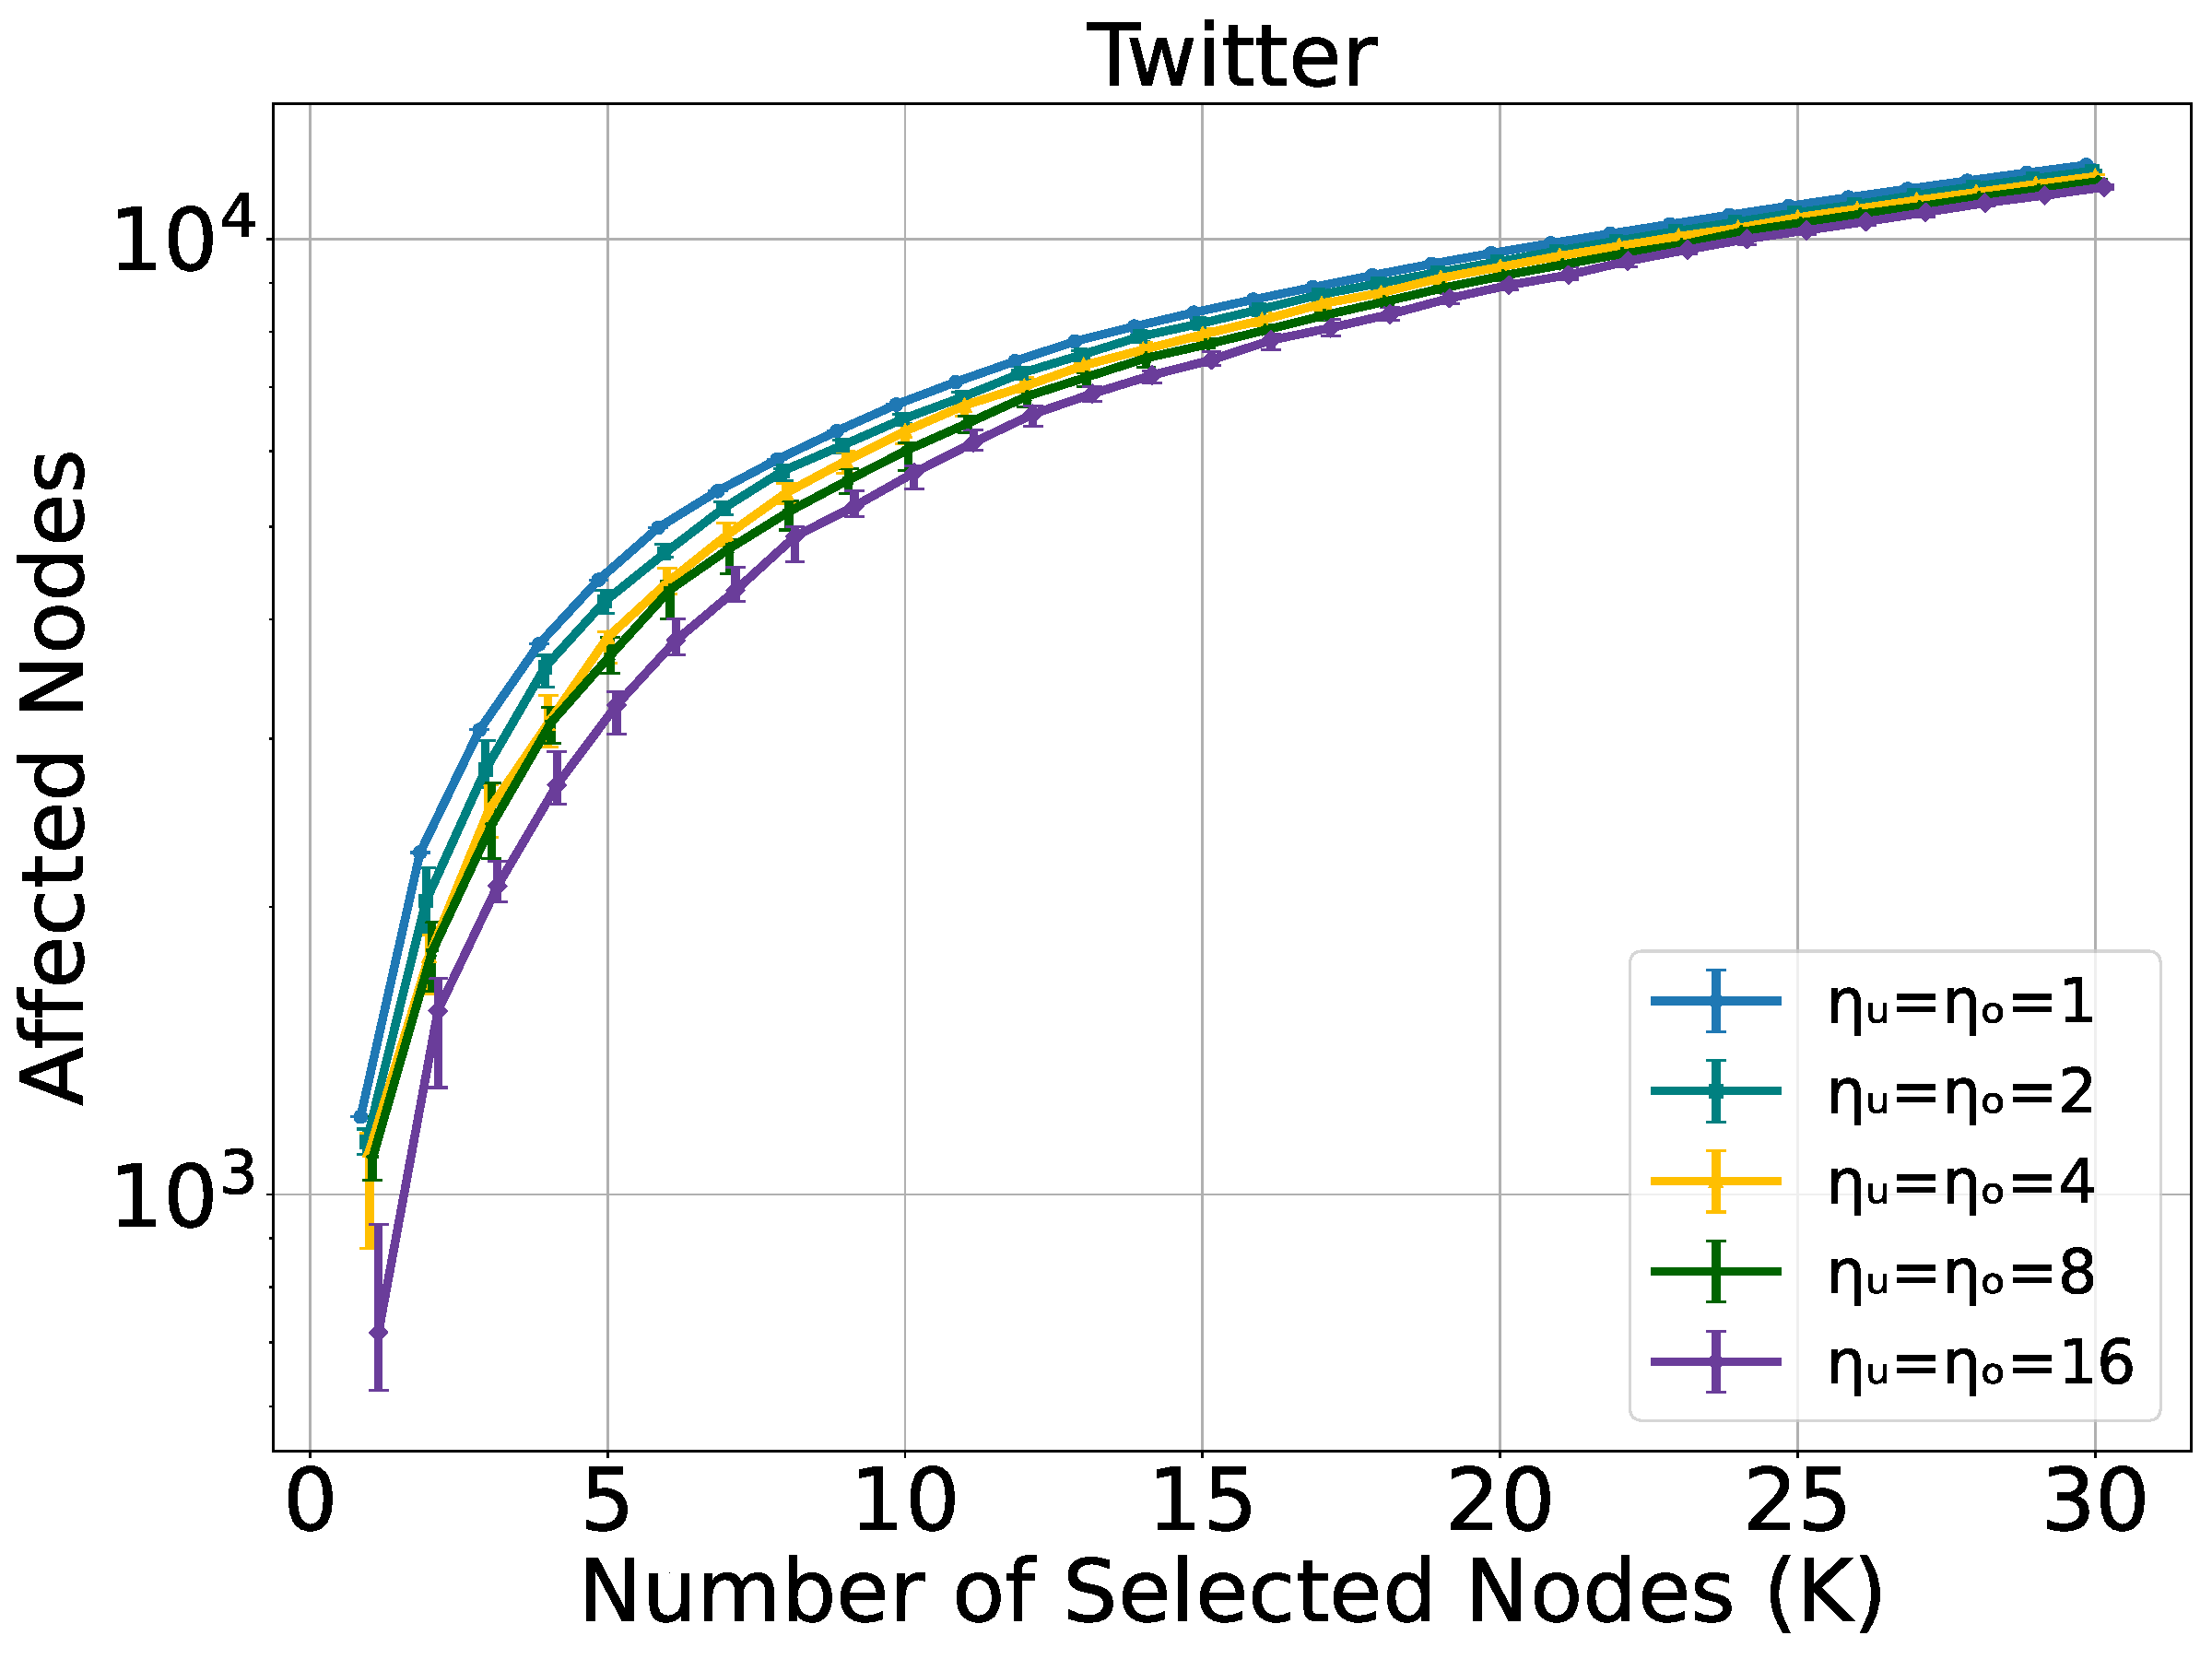
\includegraphics[width=\linewidth]{Figures/GraphExperiment/Errors/new/error_twt.pdf}
%         \label{fig:error_twt}
%     \end{minipage}\hfill
%     \begin{minipage}{0.48\columnwidth}
%         \centering
%         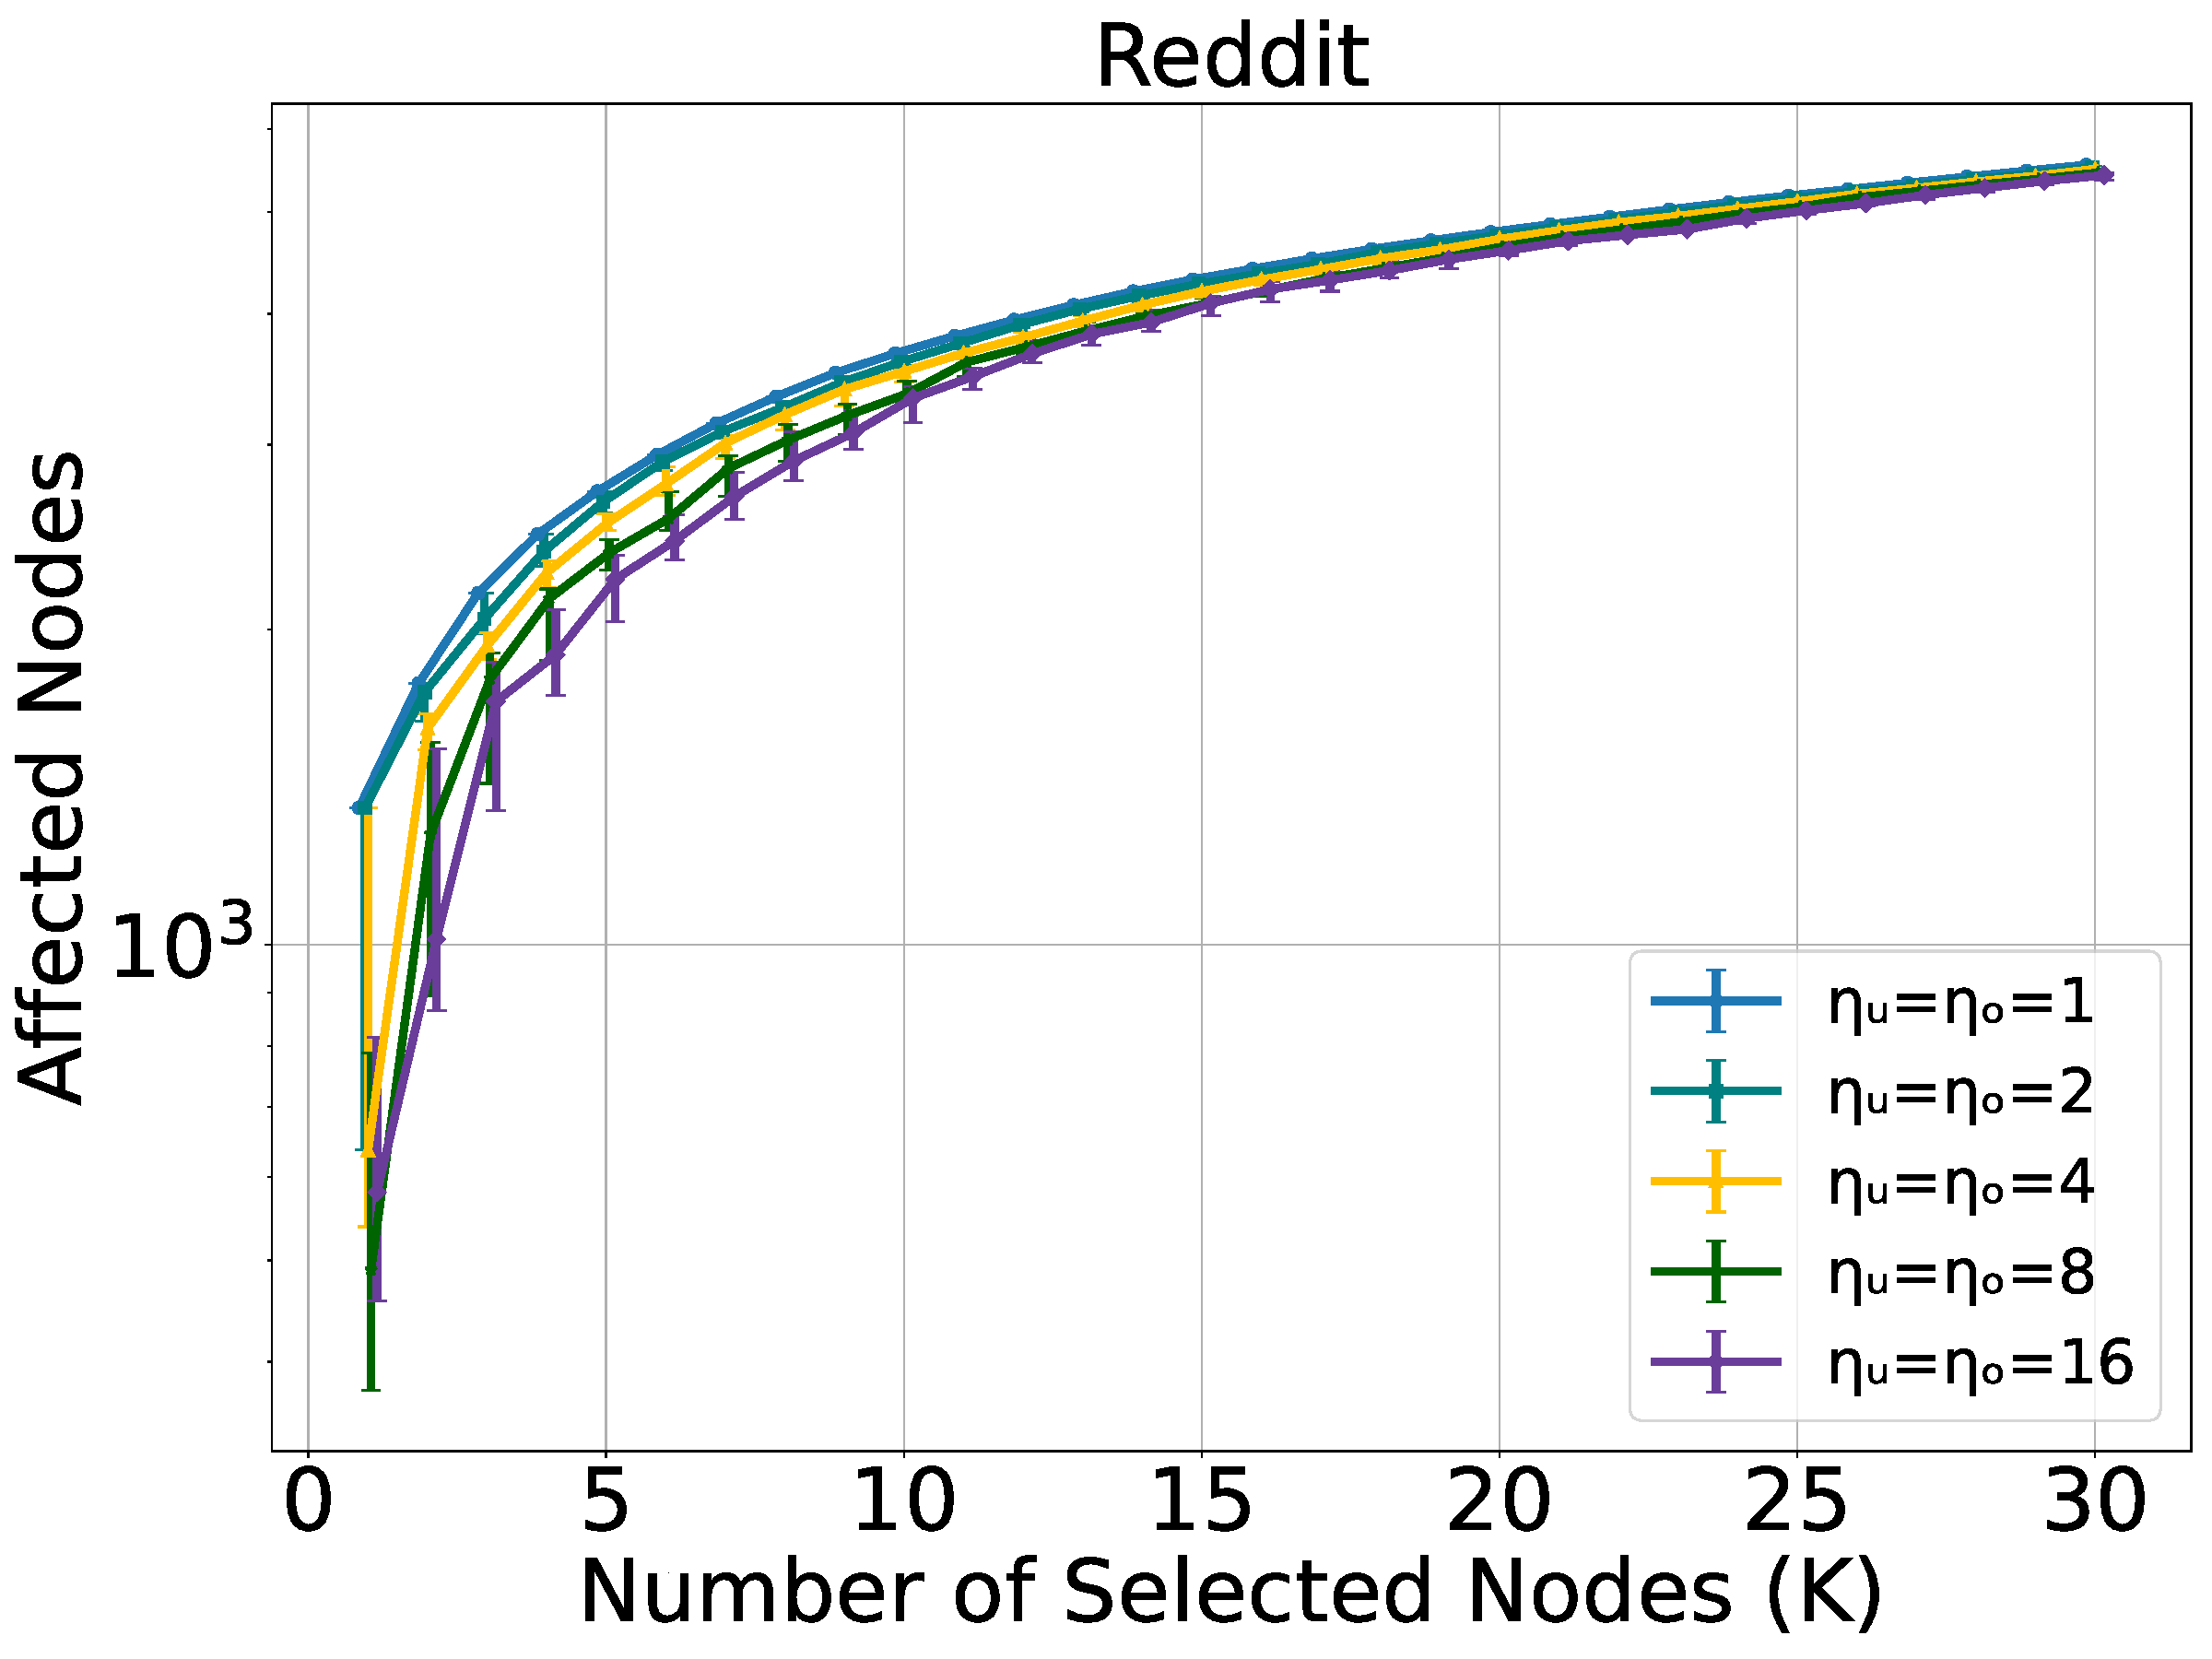
\includegraphics[width=\linewidth]{Figures/GraphExperiment/Errors/new/error_rdt.pdf}
%         \label{fig:error_rdt}
%     \end{minipage}\hfill
%     % Second row
%     \vspace{0.3cm} % Adjust the space between rows as needed
%     \begin{minipage}{0.48\columnwidth}
%         \centering
%         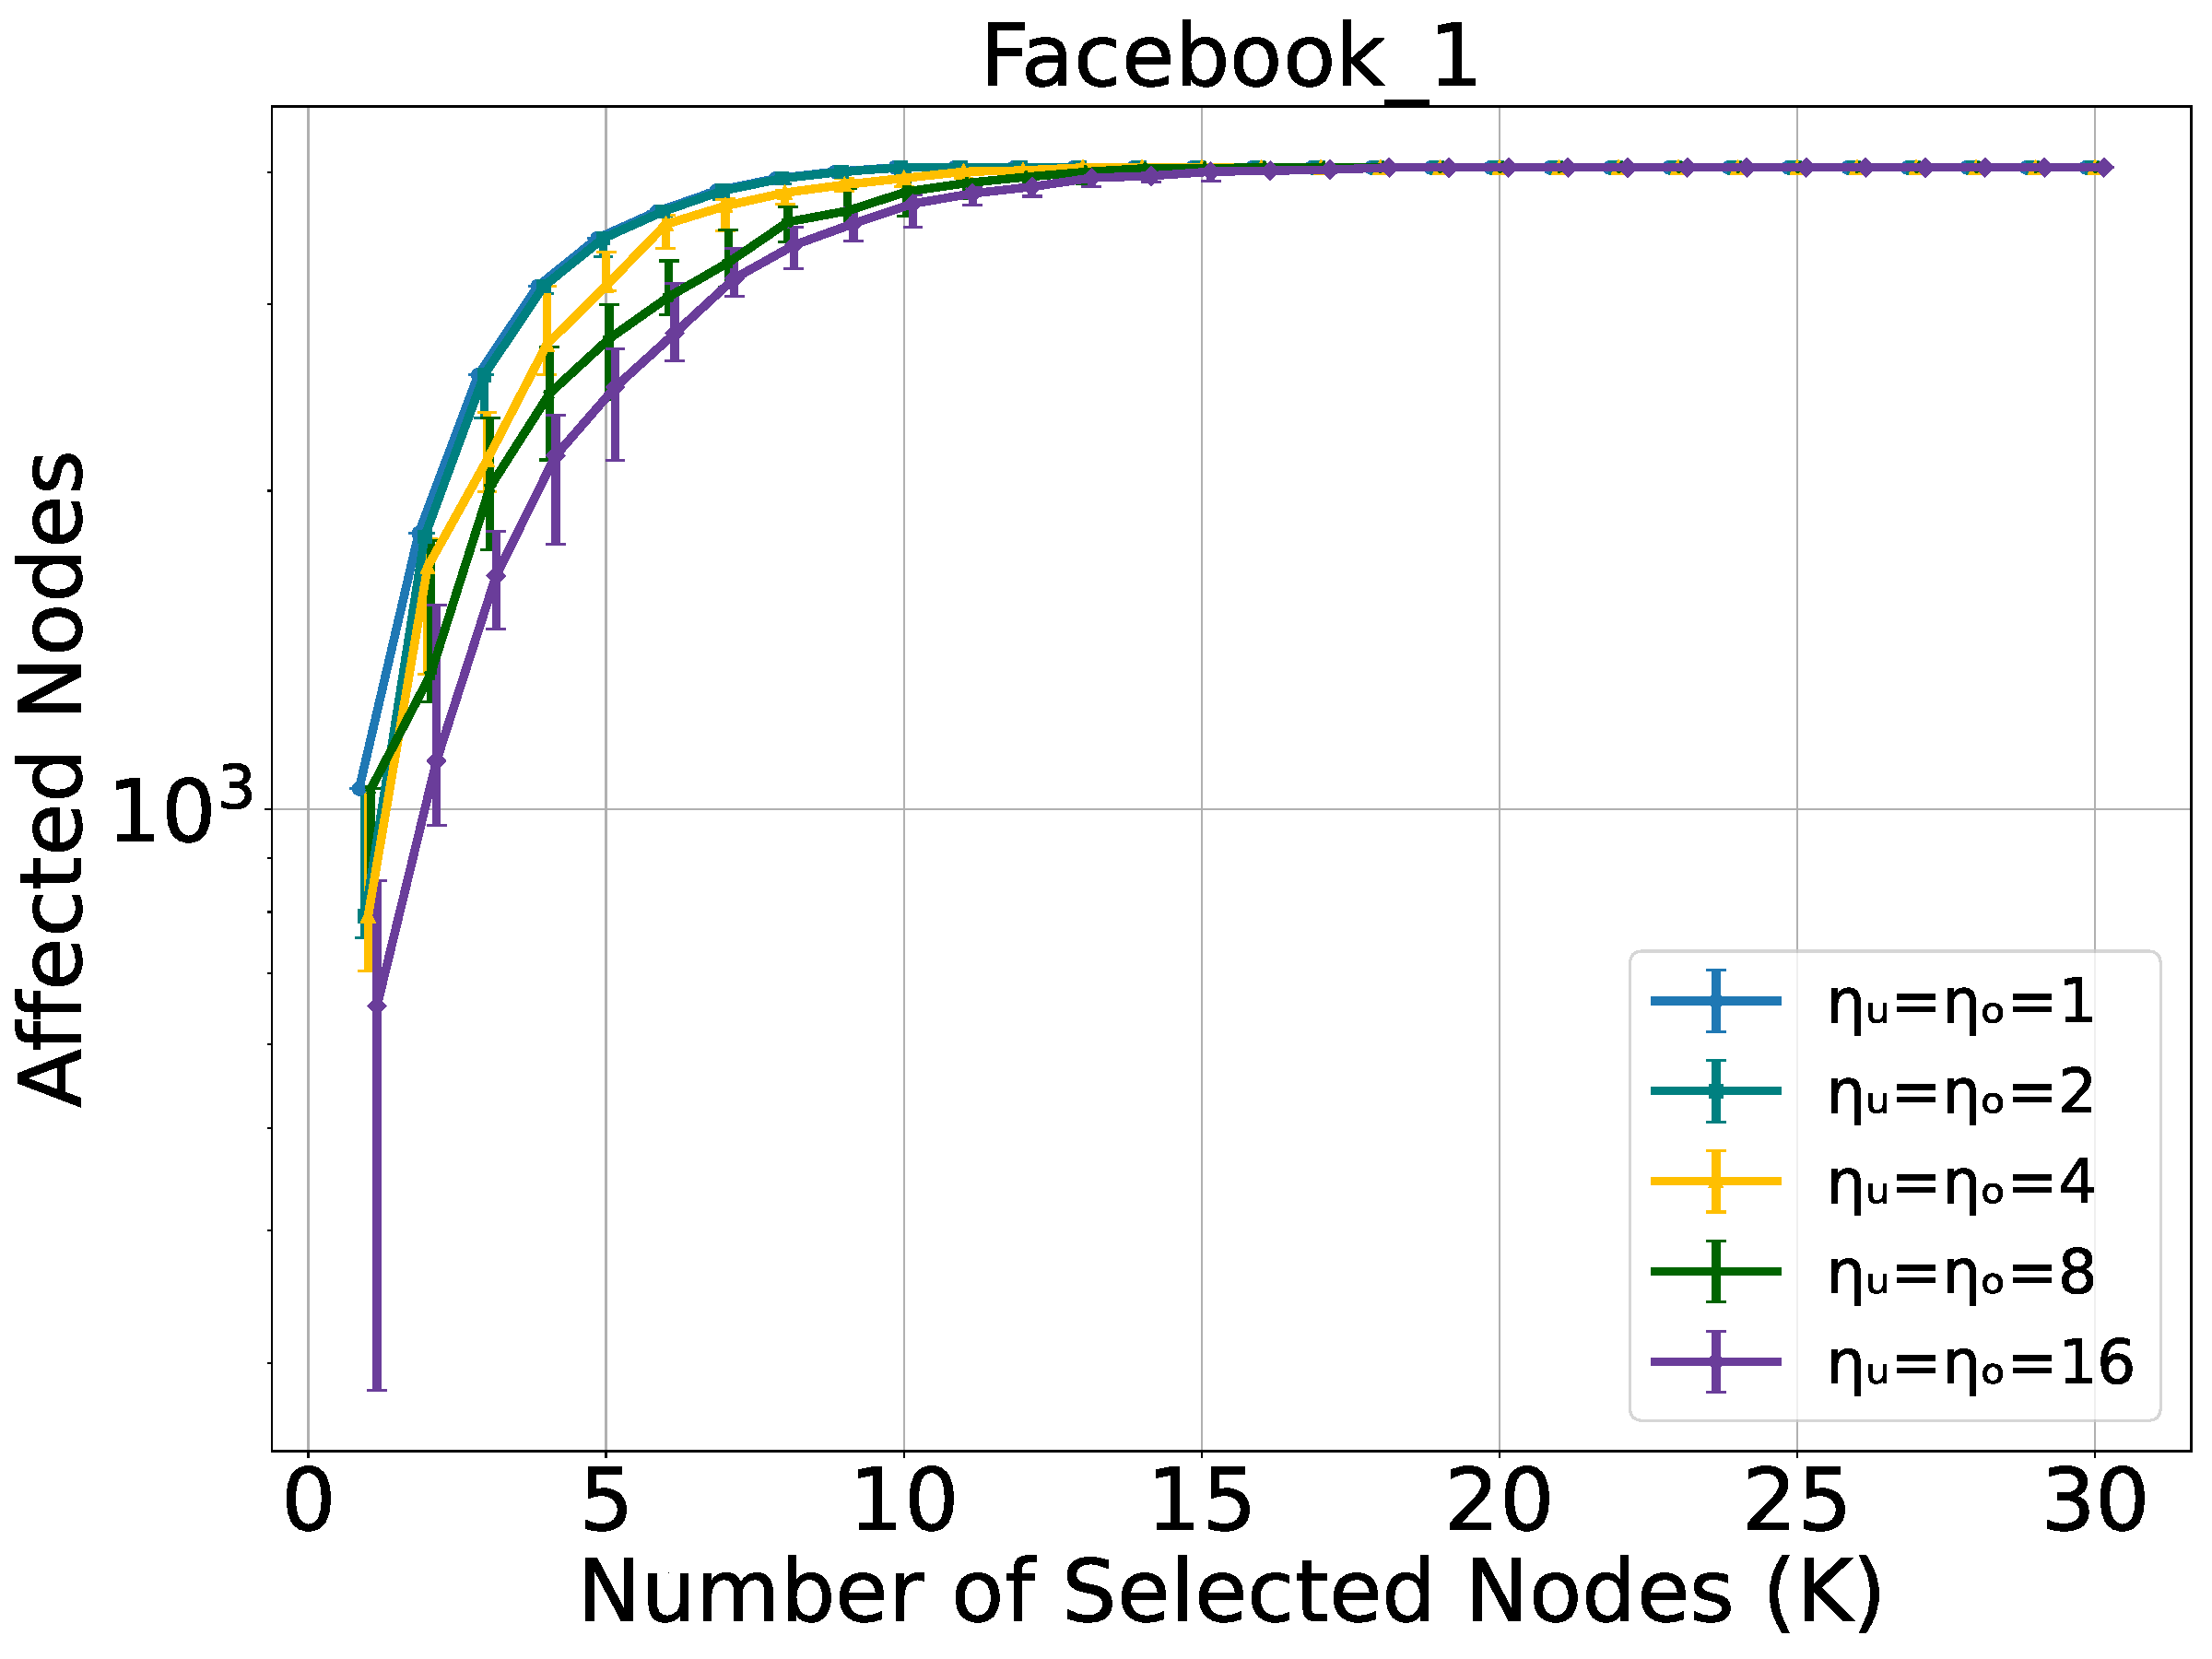
\includegraphics[width=\linewidth]{Figures/GraphExperiment/Errors/new/error_fb1.pdf}
%         \label{fig:error_fb1}
%     \end{minipage}\hfill
%     \begin{minipage}{0.48\columnwidth}
%         \centering
%         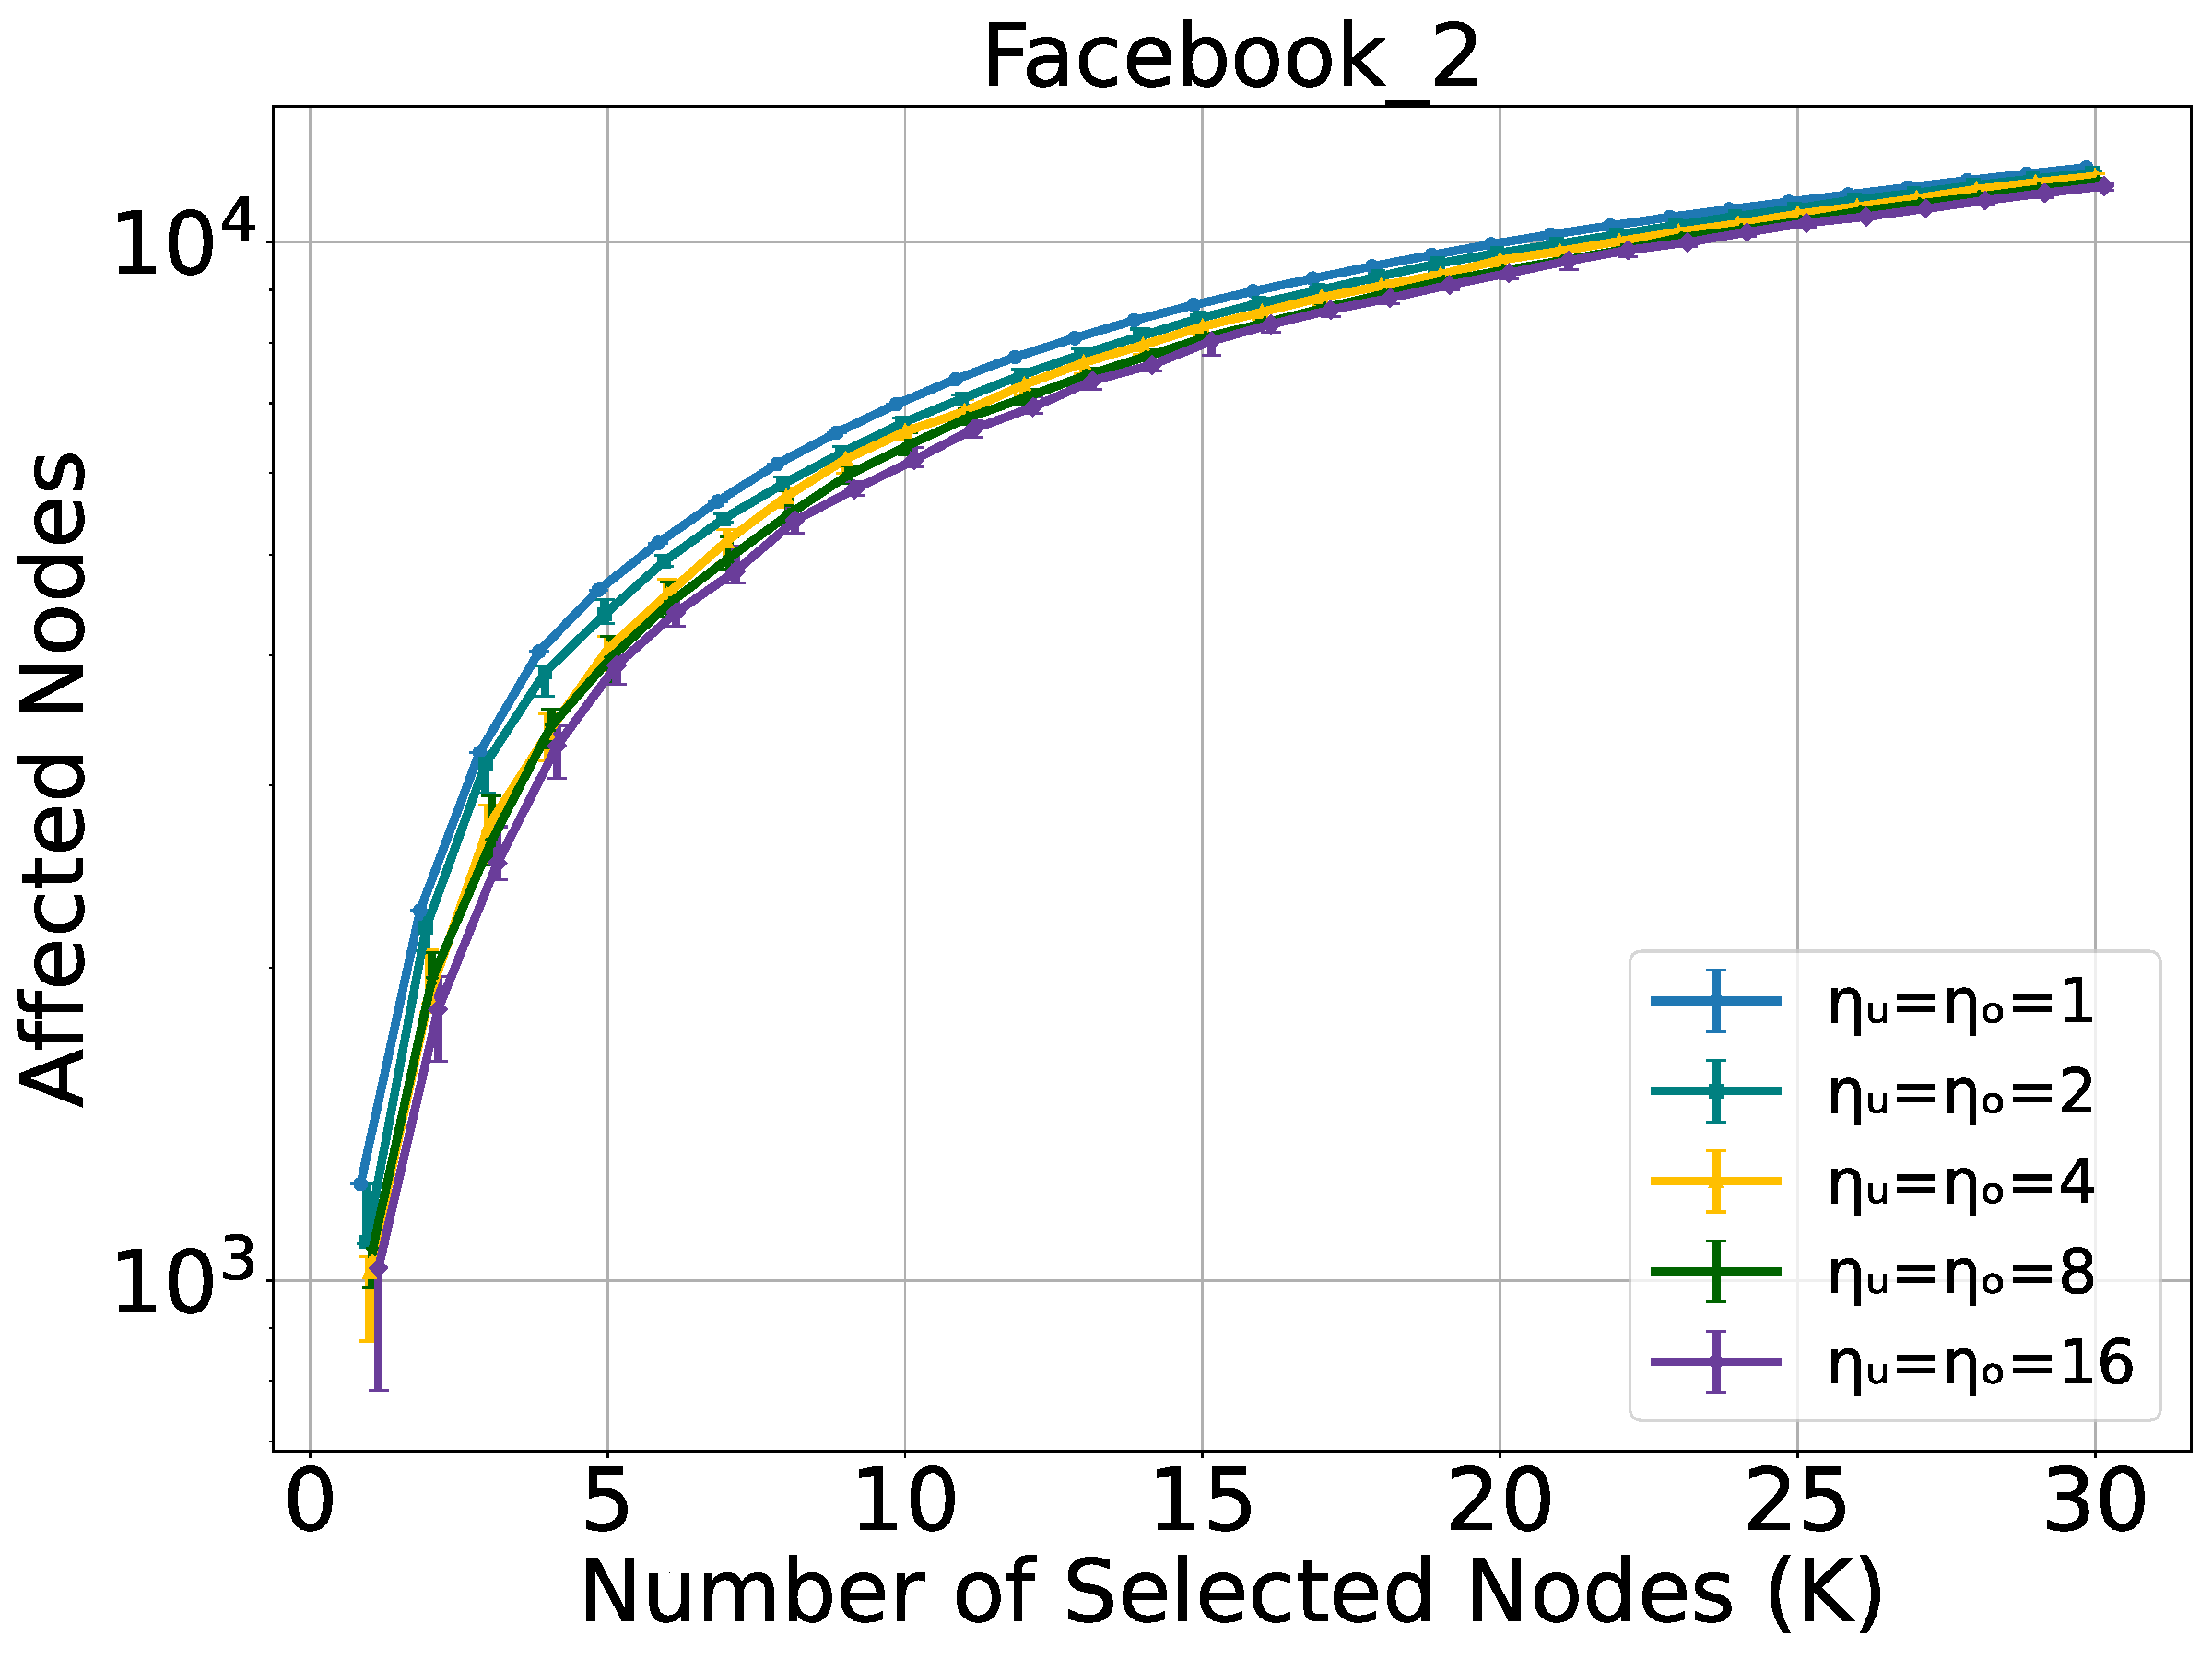
\includegraphics[width=\linewidth]{Figures/GraphExperiment/Errors/new/error_fb2.pdf}
%         \label{fig:error_fb2}
%     \end{minipage}
%     \caption{Affected nodes with an increasing $K$ by SOP-Greedy with $\eta \in [1, 256]$.}
%     \label{fig:graph_error}
% \end{figure}


%Figure \ref{fig:2stp} presents the comparisons between five methodologies: Greedy, SOP-Greedy, RSOP-Greedy, Random, and Weighted Random selection. 
%We only retain 1000 nodes with the largest degrees from each dataset since the complexity of RSOP-Greedy is $O(N^R)$, where $N$ is the number of nodes in the network. Handling large-scale networks makes RSOP-Greedy too slow. 
%Additionally, we perform experiments comparing the other methodologies (excluding RSOP-Greedy) on the large-scale networks. The results of these experiments are shown in Appendix \ref{appendix:large-scale}. 

\textbf{Results.} 
Figure \ref{fig:2stp} shows the empirical performance ratios of different algorithms across four networks with various $K$; the empirical performance ratio is defined as $\frac{f(S_{A})}{\text{OPT}}$, where $S_{A}$ denotes the value of the solution outputted by algorithm $A$ and OPT the (estimated) optimal value. The value of OPT is exact when $K = 1$; for $K > 1$, it is estimated by the solution of the greedy algorithm (with complete information) divided by $1 - e^{-1}$, representing an upper bound for the optimum. Thus, the performance ratios are a lower bound of the actual performance ratios. The empirical performance ratios of the predictive greedy consistently exceed the theoretical bounds, showing the pessimism in our theoretical results and the potential of the proposed algorithm being comparable to optimum in practice. The y-axis is on a logarithmic scale to clarify comparison. Greedy consistently achieves the strongest performance due to complete information. The performance differences between SOP-Greedy and RSOP-Greedy seem insignificant, but Figure \ref{fig:RSOP_C} provides experimental results highlighting their differences. In Figure \ref{fig:2stp}, both exhibit slightly lower performance than Greedy. However, the advantage of Greedy vanishes quickly as $K$ increases. All greedy-based algorithms observe significant advantages over Weighted Random and Random. 




Figure \ref{fig:network visualisation} shows a visualization of the node selection. 
Figure \ref{fig:graph error} presents the performance of SOP-Greedy under different prediction errors. The performance degrades as errors increase, but the disparity diminishes as $K$ increases. We observe that, even under unreasonably large errors, the performance of predictive greedy is competitive even to Greedy with complete information, showing consistency and robustness to the prediction error.


Figure \ref{fig:RSOP_C} shows additional experimental results that compare SOP-Greedy and RSOP-Greedy under various $\eta_u$ and $\eta_o$. The y-axis represents the performance ratio, calculated in the same manner as in Figure \ref{fig:2stp}. Their performance is comparable under accurate predictions. However, as $\eta_u$ and $\eta_o$ increase, RSOP-Greedy demonstrates clear advantages over SOP-Greedy under the same prediction quality. 


\begin{figure}[t]
    \centering
    % First figure
    \begin{minipage}{0.485\textwidth}
        \centering
        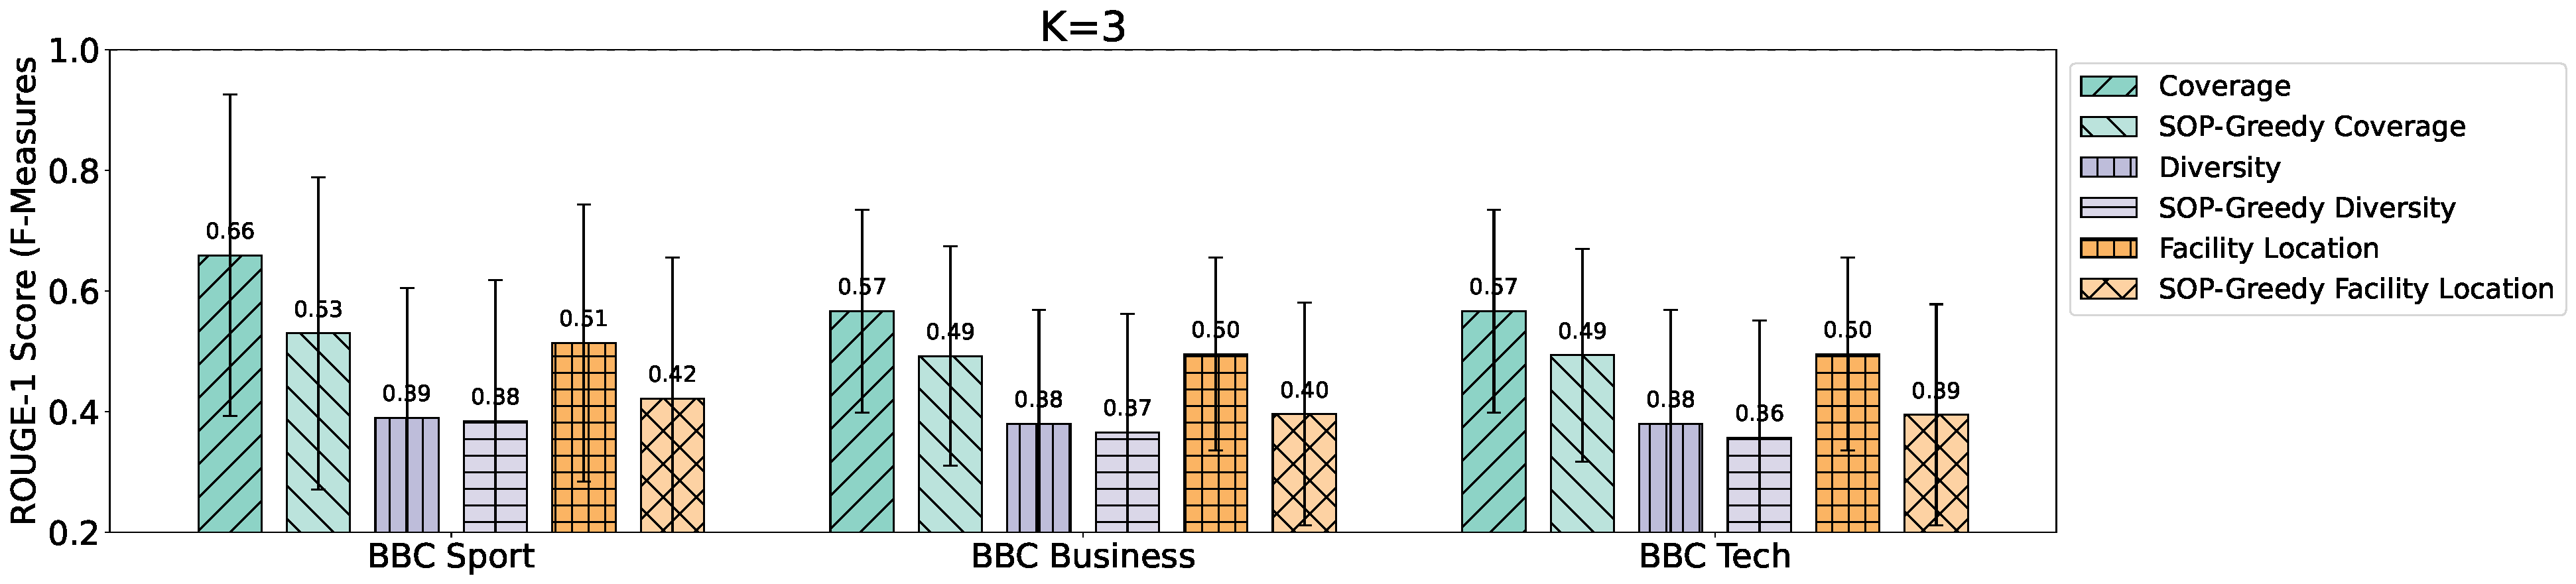
\includegraphics[width=\linewidth]{Figures/experiment 3/bbc_k3.pdf}
        %\\{\tiny (a)}
        \label{fig:bbc_k3_rouge_1}
    \end{minipage}\hfill
    \begin{minipage}{0.485\textwidth}
        \centering
        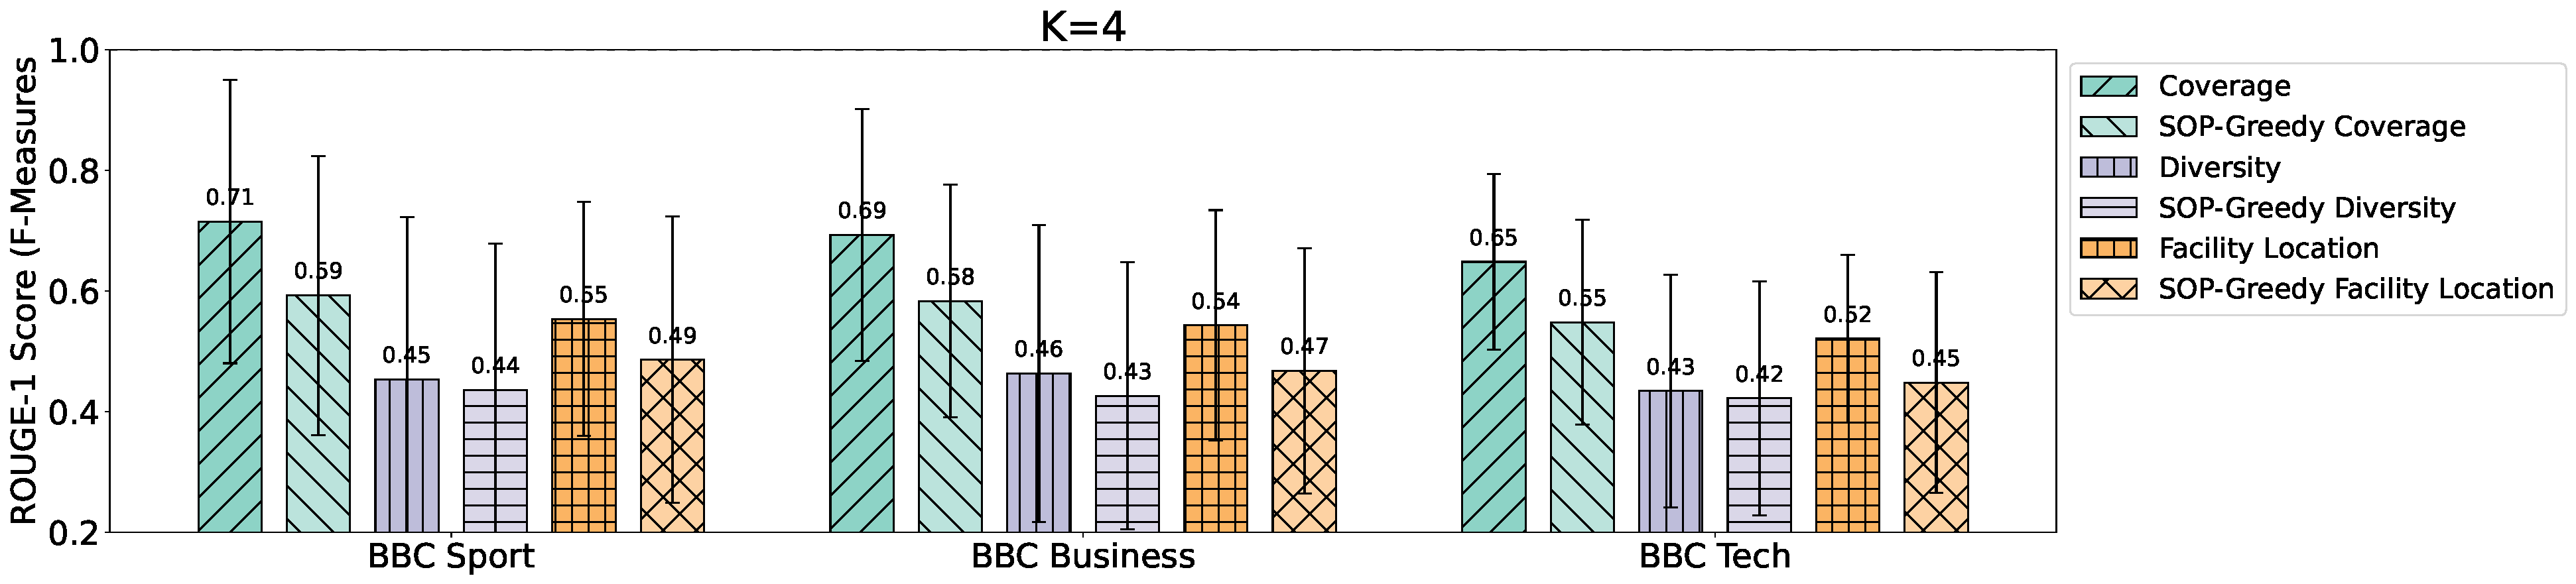
\includegraphics[width=\linewidth]{Figures/experiment 3/bbc_k4.pdf}
        \label{fig:bbc_k4_rouge_1}
    \end{minipage}\hfill
    % Second figure
    \begin{minipage}{0.485\textwidth}
        \centering
        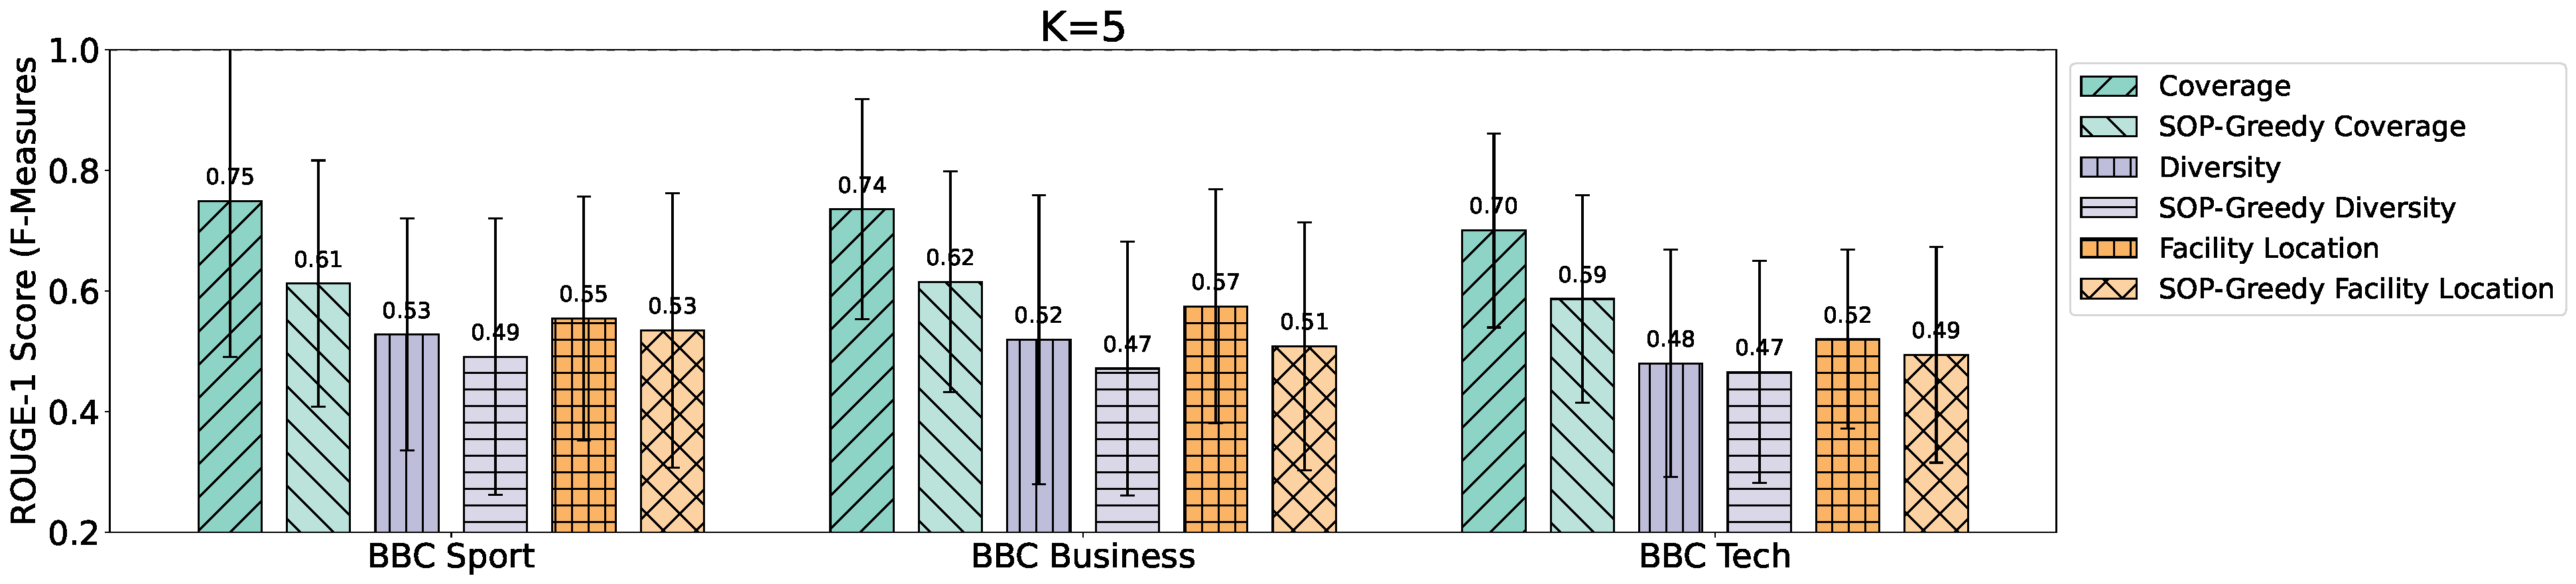
\includegraphics[width=\linewidth]{Figures/experiment 3/bbc_k5.pdf}
        \label{fig:bbc_k5_rouge_1}
    \end{minipage}

    \caption{ROUGE‐1 scores (F‐measure) across three BBC news—sport, business, and tech—under $K \in [3, 5]$. The results highlight how each approach scales with $K$ and differs by BBC news categories \cite{yadav2022extractive}.}
    \label{fig:BBCnews}
\end{figure}




\begin{figure*}[ht!]
    \centering
    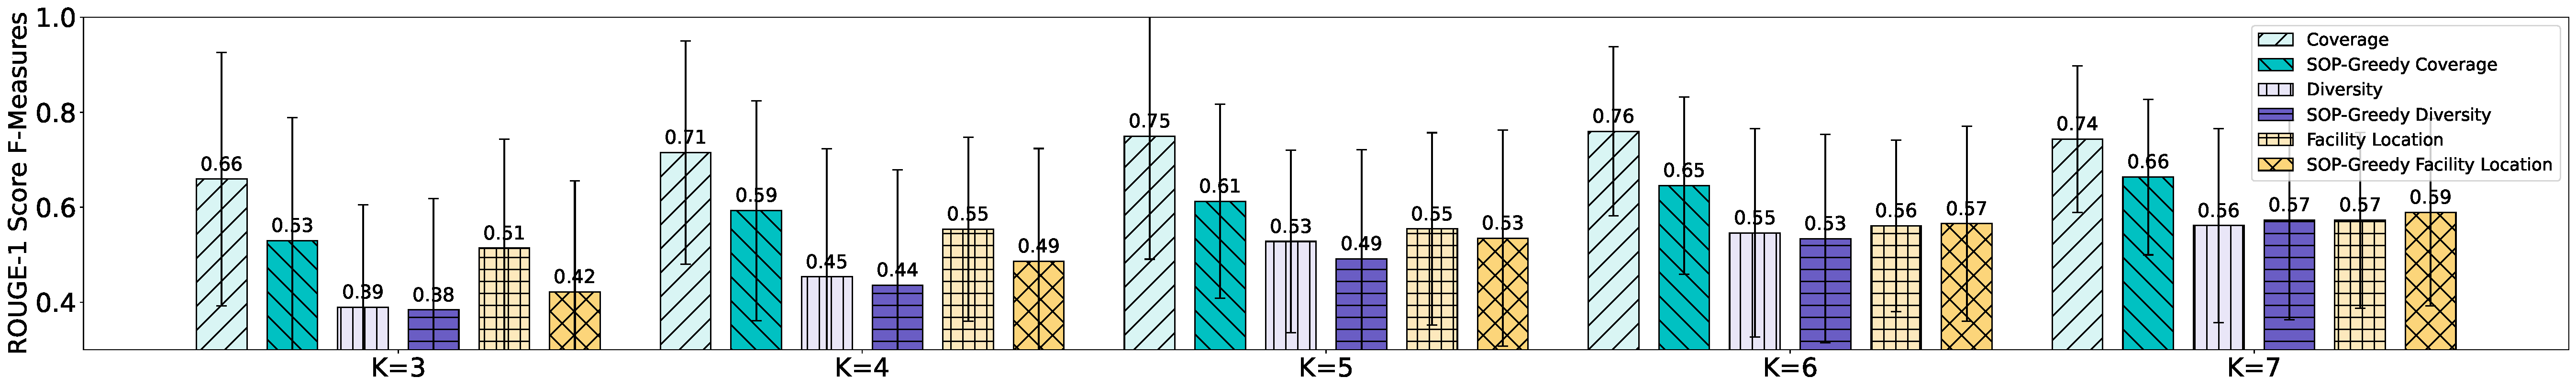
\includegraphics[width=\textwidth]{Figures/experiment 3/sports.pdf}
    \label{fig:dummy-ref}
    \caption{Rouge-1 scores for the greedy and SOP-Greedy under $K \in [3, 7]$ on the BBS news sport \cite{minaee2021deep}. The IQRs of the results are reported.}
    \label{fig:text-summary}
    \vspace{-15pt}
\end{figure*}

\subsection{Text summarization} \label{subsec:text-summarization}


\begin{figure}[t]
    \centering
    % First figure
    \begin{minipage}{0.48\textwidth}
        \centering
        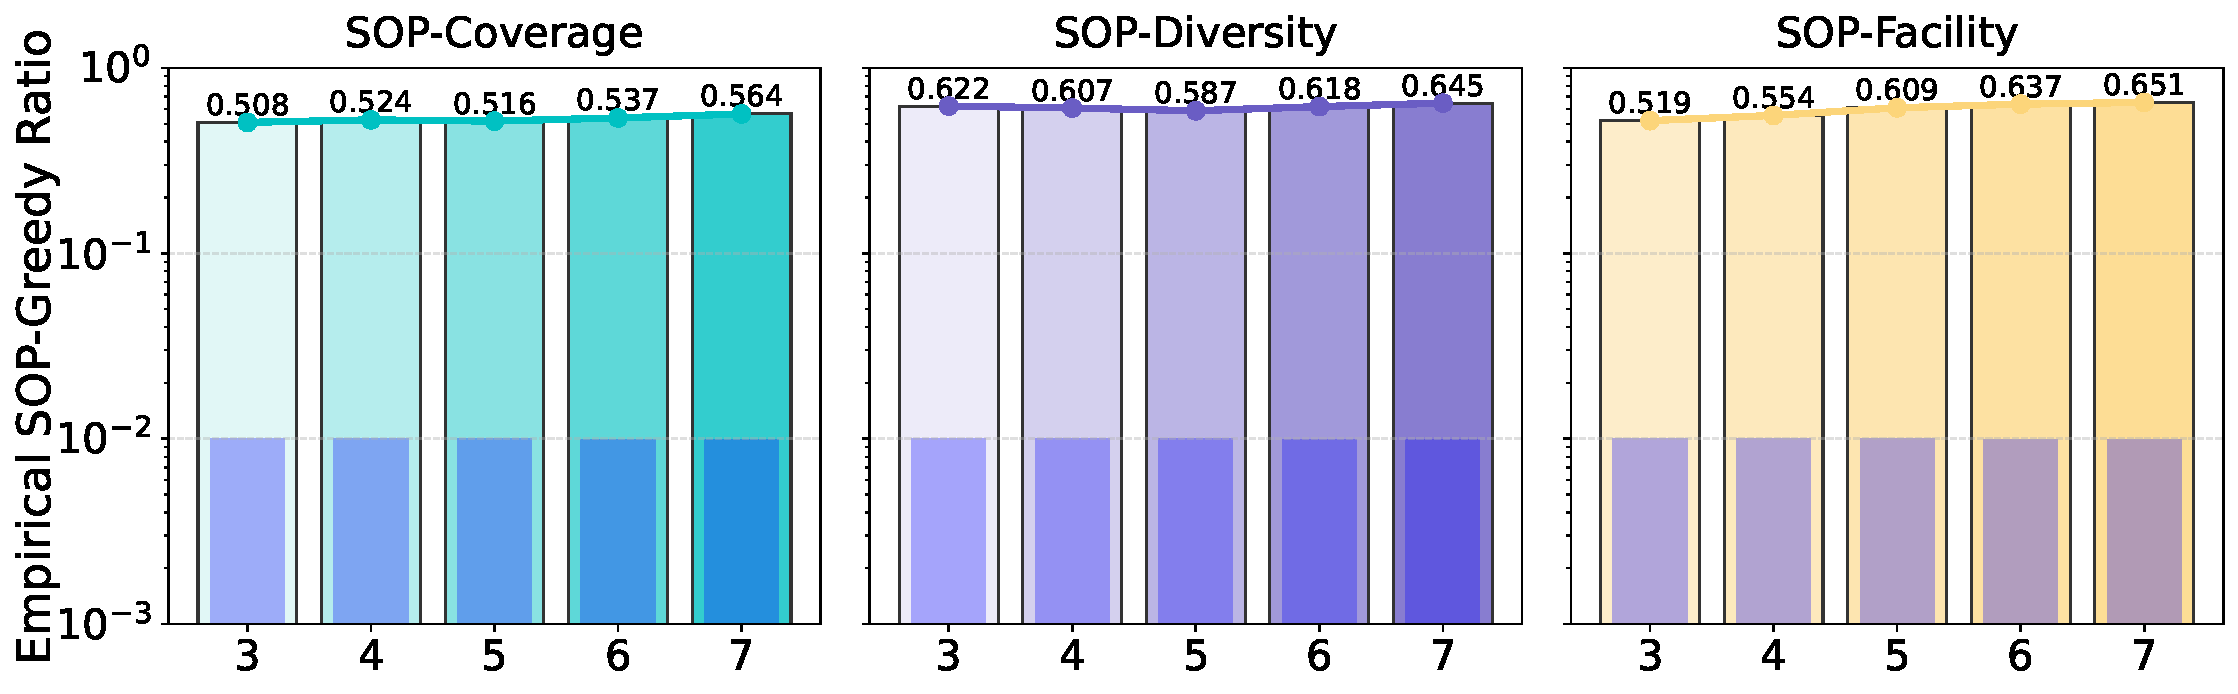
\includegraphics[width=\linewidth]{Figures/experiment 3/performance_ratio.pdf}
        %\\{\tiny (a)}
        \label{fig:sub}
    \end{minipage}\hfill
    
    \caption{Empirical SOP-Greedy performance ratios for text summarization under three submodular objectives—coverage, diversity, and facility—with $K \in [3, 7]$ on the BBS news sport \cite{minaee2021deep}. The bottom shaded bars represent the theoretical bounds.}
    \vspace{-14pt}
    \label{fig:text-ratio}
\end{figure}



This experiment considers text summarization, which has been formulated and proven as submodular optimization under cardinality constraint \cite{lin2011class}. Let $V$ be a set of $n$ tokens, which could be phrases or paragraphs, labeled as $1, \dots, n$, i.e., $V = \{1, \dots, n\}$. Our task is to find a set $S \subseteq V, |S| \leq K$, so that $S$ is a summary of $V$ with the highest quality measured by some score function $f: 2^V \rightarrow \mathbb{R}$. The literature on text summarization proposes many submodular score functions that are widely used. We consider three of them: \textit{coverage}, \textit{diversity}, and \textit{facility location} \cite{lin2011class}. 
Coverage measures information covered and is defined as $f_{\text{cov}}(S) = \sum_{i \in V} \min \left\{\sum_{j \in S} w_{i, j}, \alpha \sum_{k \in V} w_{i, k}\right\}$, where $w_{i, j}$ is the similarity between tokens $i$ and $j$, and $\alpha$ a parameter controlling the saturation point of coverage. 
Diversity measures diversity of the information and is defined as $f_{\text{div}}(S) = \sum_{k=1}^{K} \sqrt{\sum_{j \in S \cap P_k} \frac{1}{N} \sum_{i \in V} w_{i, j}}$, where $S \cap P_k$ denotes the intersection of $S$ with a partition $P_k$ of $V$. 
Facility location measures representativeness to $V$ and is defined as $f_{\text{loc}}(S) = \sum_{i \in V} \max_{j \in S} w_{i, j}$. The text summarization problem can be cast as the following optimization. 

\[ \max_{S \subseteq V} \{f(S) : |S| \leq K, f ~\text{submodular} \} \]

There is no universally agreed $f$. However, it is generally assumed that $f$ is non-decreasing and submodular due to information coverage and redundancy of a summary \cite{lin2011class}, and $f$ correlates well with the ROUGE‐1 score. Though $f$ is inaccessible, practitioners may use a sensible heuristic, such as some variants of the above-mentioned score functions, as the predictor $\tilde{f}$ to approximate ROUGE-1.


%The aim of the third experiment is to extract the most essential information from a lengthy text or collection of documents and present them in a condensed form. 
%We address the issue of extractive summarization as a submodular function maximisation under cardinality constraints, aligning with the methodology given in \cite{lin2011class}. %For monotone submodular functions, greedy algorithms theoretically guarantee near-optimal solutions.

%\textbf{Submodular objective functions.} Every element in our document set, $V = \{1, \dots, n\}$, stands for a separate piece of text, such as a phrase or paragraph, and is used in the context of extractive summarization. 
%Finding a subset $S \subseteq V$ that maximises the summarization quality $F(S)$ while keeping $|S| \leq K$. 
%Here, $F$ is a submodular function that encompasses important factors like coverage, diversity, and facility location, three crucial components in text summarization. 
\begin{comment}
Firstly, the Coverage Function $\mathcal{L}_1(S)$ \cite{lin2011class}, considered as $F_{\text{cov}}(S)$ in our experiment, for maximizing the total information covered by the summary is defined as:
\[
F_{\text{cov}}(S) = \sum_{i \in V} \min \left\{\sum_{j \in S} w_{i, j}, \alpha \sum_{k \in V} w_{i, k}\right\},
\]
where $w_{i, j}$ represents the weight or similarity between elements $i$ and $j$, and $\alpha$ is a parameter to control the saturation point of coverage.

The second submodular function is Diversity Function, $R_1(S)$ \cite{lin2011class}, considered as $F_{\text{div}}(S)$, aims to ensure the summary includes diverse aspects from the document set, expressed as:
\[
F_{\text{div}}(S) = \sum_{k=1}^{K} \sqrt{\sum_{J \in S^{\perp} P_{k}} \frac{1}{N} \sum_{i \in V} w_{i, J}},
\]
where $S^{\perp} P_{k}$ denotes the complement of $S$ within a partition $P_k$ of $V$.

Finally, the Facility Location Function\cite{ahmed2011maximizing}, $F_{\text{loc}}(S)$, focuses on maximizing the representativeness of the subset $S$ for the entire document set:
\[
F_{\text{loc}}(S) = \sum_{i \in V} \max_{j \in S} w_{i, j},
\]
Where the similarity between document $i$ and phrase $j$ in the subset $S$ is denoted by $w_{i, j}$.
\end{comment}

\begin{comment}
Then we modify the standard greedy submodular maximization algorithm by incorporating a prediction error term:

    \[
    f_{\text{error}}(S) = f(S) + \epsilon(S), \quad \epsilon(S) \sim \mathcal{U}(-\log \eta_u, \log \eta_o),
    \]
where $\epsilon(S)$ models the error as a uniformly distributed variable.
\end{comment}

\textbf{Experimental set-up.}
We collect texts from BBC news \cite{bbcnews_dataset} to form three datasets each including 100 articles under sport, business, and tech categories. Every article is tokenized into sentences. Every article has its summary from BBC news. We evaluate the summarization algorithm using the original summary with Rouge-1 score F-measure, a metric that balances information relevance and accuracy. We implement the greedy algorithm and predictive greedy. The greedy algorithm uses coverage with $\alpha$ = 1, diversity with number of clusters = 2, and facility location as heuristic to determine the summary; the feature extraction step employs IDF-weighted term vectors; the predictive greedy uses an erroneous heuristic. We want to see how the errors in the heuristic affect the quality of the summary measured by Rouge-1 score against the original summary. 
The algorithm is evaluated with different heuristics; the cardinality constraint $K$ ranges from 3 to 7; the prediction error is set to $\eta = 100$ ($\eta_u = \eta_o = 10$). The experiments are conducted with Intel Core 12600KF, RAM 16GB, and GPU Nvidia Geforce RTX 3070, 8GB VRAM. 


\textbf{Results.}
Across the three BBC news categories, as shown in Figure \ref{fig:BBCnews}, coverage and facility consistently achieve higher ROUGE-1 scores than diversity, while predictive greedy behaves similarly to greedy algorithms with complete information. Figure \ref{fig:text-summary} shows the Rouge-1 scores for three submodular heuristics—coverage, diversity, and facility—under varying $K$ on the BBS news sport dataset. The performance of the greedy and predictive greedy converges as $K$ increases, showing the consistency and robustness of the predictive greedy under large $K$. Diversity is the worst among the three heuristics for summarization under small $K$. This is intuitive, as information coverage is the primary concern and diversity is secondary. Figure \ref{fig:text-ratio} shows the empirical performance ratios of SOP-Greedy, estimated with OPT set to $\min \{ 1, \frac{f(S_{\text{greedy}})}{1 - e^{-1}}\}$, where $S_{\text{greedy}}$ denotes the solution outputted by the greedy with complete information. The non-trivial error ($\eta_u = \eta_o = 10$) leads to minor theoretical bounds, shown in Figure \ref{fig:text-ratio} and Table \ref{tab:theoretical-bound}. The empirical performance ratios are consistently higher than the competitive ratios, showing the potential of the predictive greedy to be close to the optimum in practice. 

\begin{table}[ht!]
\centering
\caption{Competitive ratios for SOP-Greedy under varying K and $\eta_u = \eta_o = 10$.}
\label{tab:theoretical-bound}
\begin{tabular}{c|ccccc}
\hline\hline
\textbf{K} & 3 & 4 & 5 & 6 & 7 \\
\hline
\textbf{comp. ratio} & 0.009967 & 0.009963 & 0.009960 & 0.009958 & 0.009957 \\
%\textbf{K} & \textbf{SOP-Coverage} & \textbf{SOP-Diversity} & \textbf{SOP-Facility Location} \\
%\hline
%\textbf{3}   & 0.009967 & 0.009967 & 0.009967 \\
%\textbf{4}   & 0.009963 & 0.009963 & 0.009963 \\
%\textbf{5}   & 0.009960 & 0.009960 & 0.009960 \\
%\textbf{6}   & 0.009958 & 0.009958 & 0.009958 \\
%\textbf{7}   & 0.009957 & 0.009957 & 0.009957 \\
\hline\hline
\end{tabular}
\vspace{-12pt}
\end{table}

%It is observed in Figure \ref{fig:textk}: when K increases, the Rouge-1 score also improves because adding sentences in the simulated summary bring audience with valid information. 
%When K reaches a certain point, K = 5, the incremental information gain is not obvious. So, we make the subsequent plots across three news categories for K = 3, 4 and 5, which is displayed in Appendix \ref{appendix:supp-material-application3}. 
%Figure\ref{fig:overall} indicates that converge and facility location greedy have similar performance and outperform the other method. The predictive greedy has close performance with each objective method under the reasonable prediction error value. These findings support the statement that submodular functions, especially when implemented with predictive error, offer a robust structure for producing short but informative summaries. Consistent performance across different $K$ values further demonstrates how the predictive methods can be adjusted for various cardinaity constraints. 


\begin{comment}
\begin{figure}
    \centering
    \begin{subfigure}{\textwidth}
        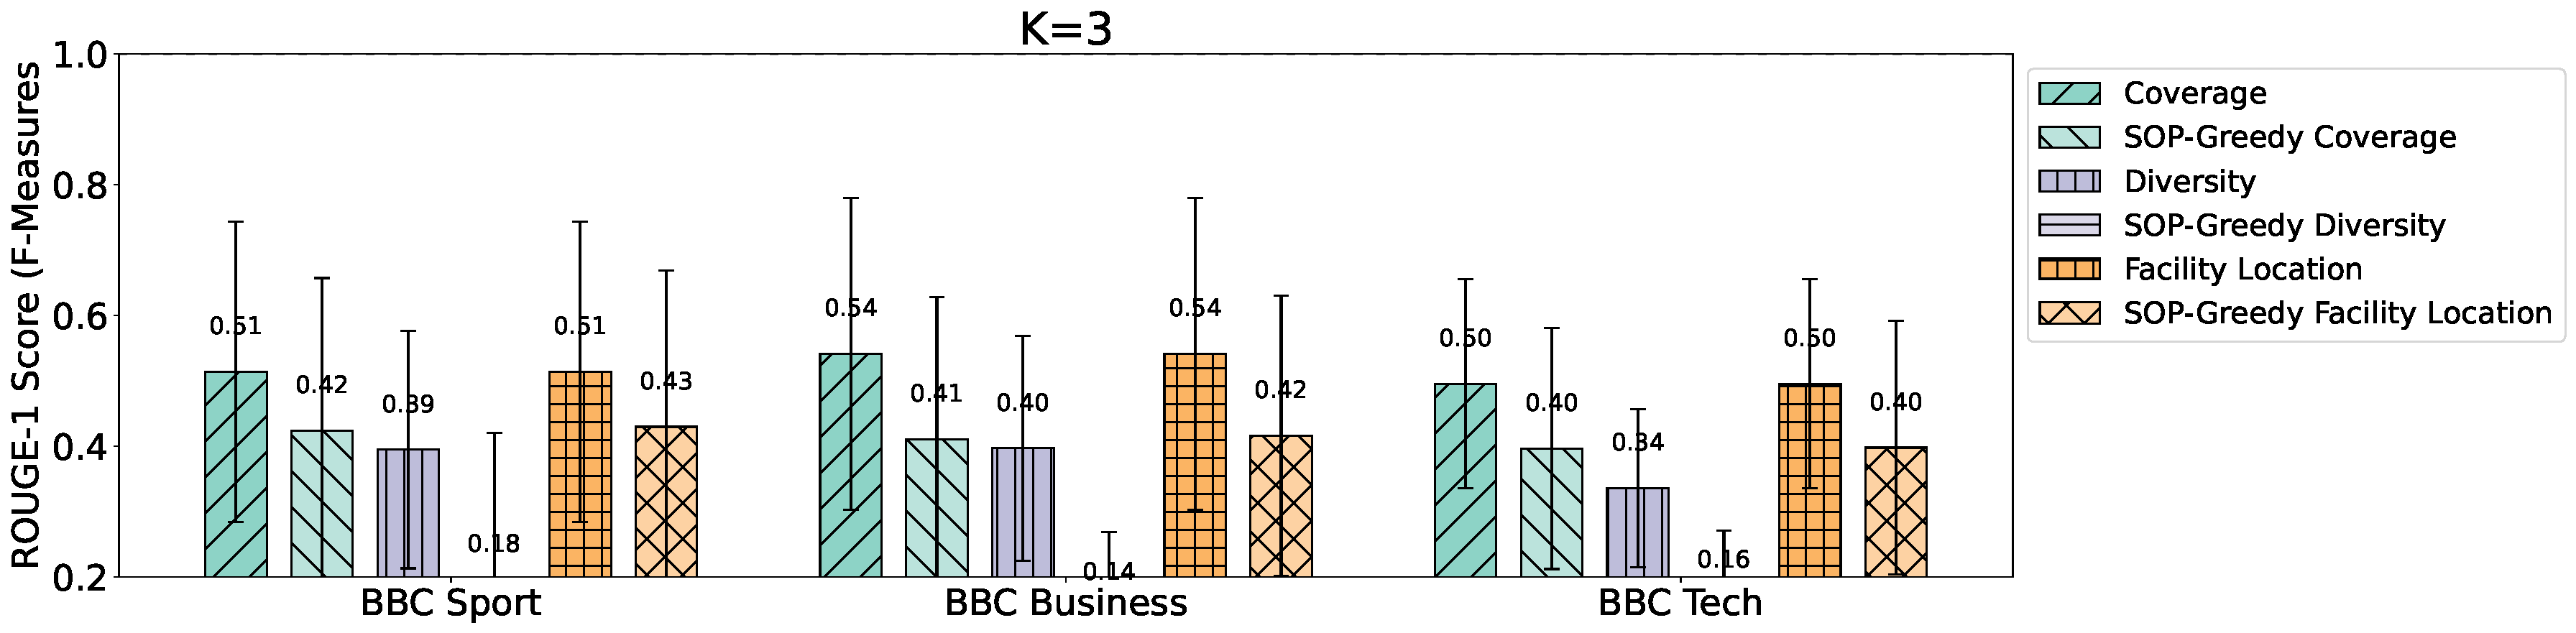
\includegraphics[width=0.65\textwidth]{Figures/experiment 3/bbcsport_k3.pdf}
    \end{subfigure}
    \begin{subfigure}{\textwidth}
        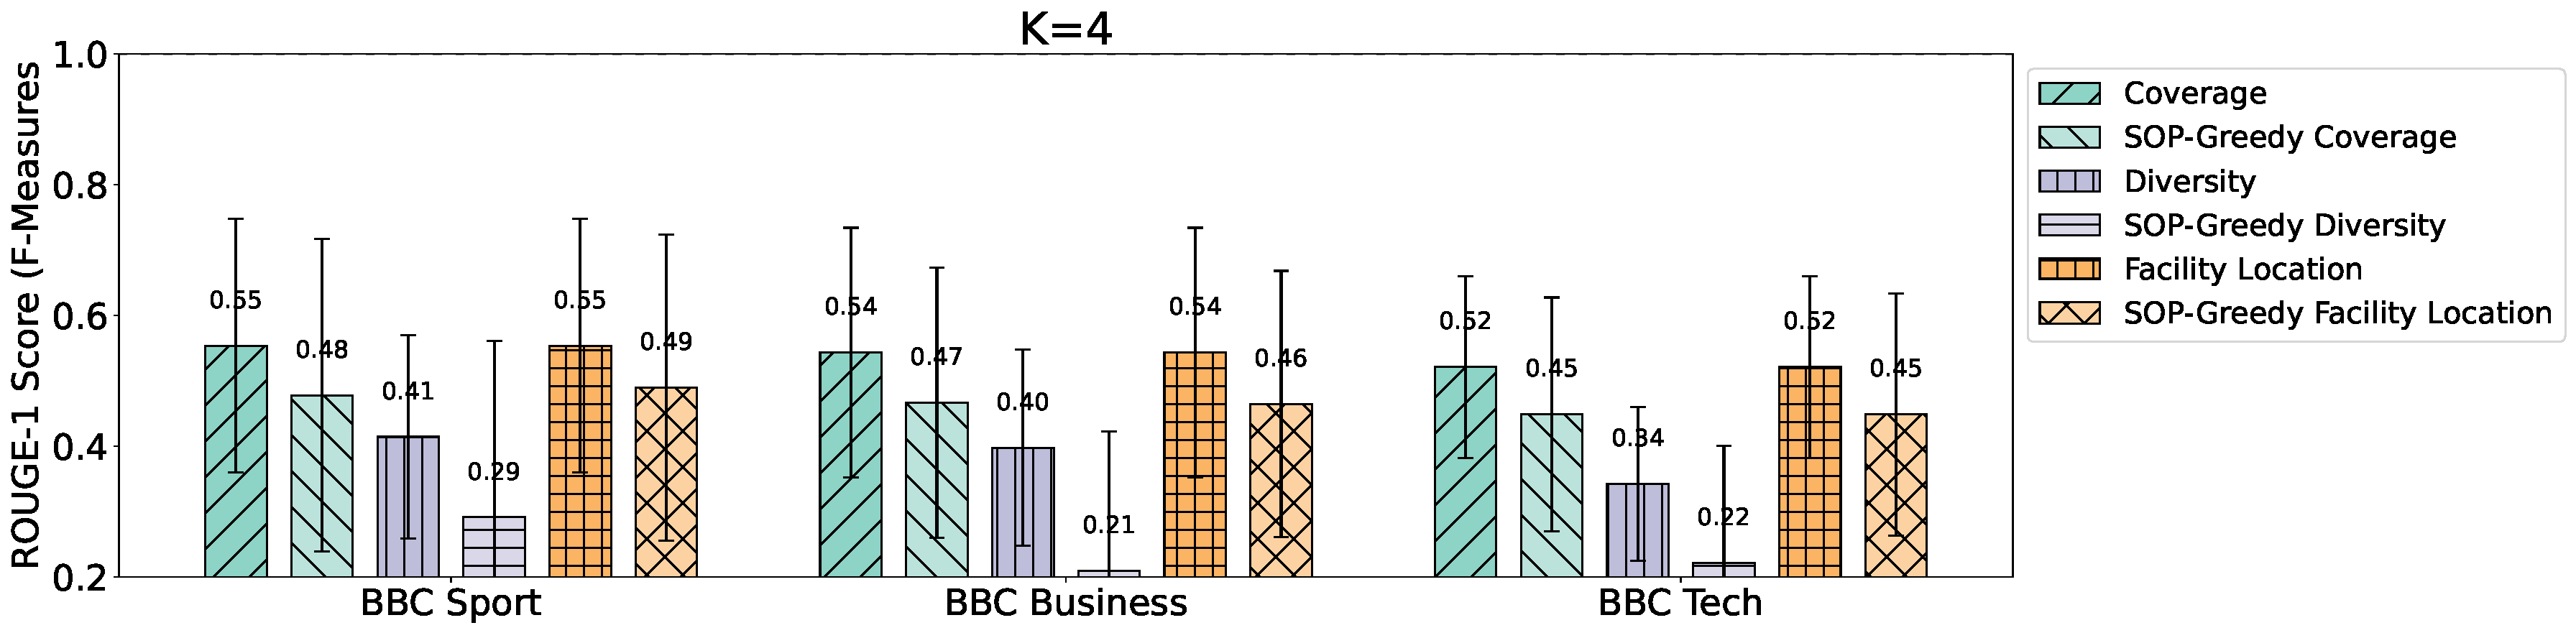
\includegraphics[width=0.65\textwidth]{Figures/experiment 3/bbcsport_k4.pdf}
    \end{subfigure}
    \caption{Overall Caption for all Plots}
    \label{fig:overall}
\end{figure}
\end{comment}


\subsection{Concluding remarks}
Our experiments show that SOP-Greedy and RSOP-Greedy are robust to prediction errors when $\eta$ is up to hundreds in real-world applications. They observe performance comparable to the greedy with complete information and smooth and graceful performance degradation as prediction errors worsen. These results also verify the theoretical guarantees, even if we use the upper bounds of OPT in the calculation. 




\section{Limitations} \label{sec:limitations}
We do not present the upper bound on the approximation ratio for the proposed problem or the tightness of our analysis. Our experiments assume independent erroneous oracles as predictors, with errors that are randomized and independent rather than adversarial. As a result, the worst-case performance of the algorithms might not be fully reflected. Additionally, erroneous oracles are not implementable in practice, as they require the exact submodular function values, which are assumed to be unknown. 


\section{Conclusions} \label{sec:conclusions}

We propose the problem of submodular optimization for an unknown function with predictions. We introduce a simple but effective error metric on the multiplicative approximation of the marginal gains. Our error metric allows the quality of algorithms to scale smoothly with the prediction error, admitting simple single-step and $R$-step greedy heuristics. We show the approximation ratios of the greedy algorithms as functions of the prediction error. Extensive experiments show that the proposed problem models real-world applications well, and the greedy algorithms observe robust performance even under large prediction errors. 


%\section*{Acknowledgments}








% if have a single appendix:
%\appendix[Proof of the Zonklar Equations]
% or
%\appendix  % for no appendix heading
% do not use \section anymore after \appendix, only \section*
% is possibly needed

% use appendices with more than one appendix
% then use \section to start each appendix
% you must declare a \section before using any
% \subsection or using \label (\appendices by itself
% starts a section numbered zero.)
%
\begin{comment}
\appendices
\section{Proof of the First Zonklar Equation}
Appendix one text goes here.

% you can choose not to have a title for an appendix
% if you want by leaving the argument blank
\section{}
Appendix two text goes here.
\end{comment}


\begin{comment}
% use section* for acknowledgment
\ifCLASSOPTIONcompsoc
  % The Computer Society usually uses the plural form
  \section*{Acknowledgments}
\else
  % regular IEEE prefers the singular form
  \section*{Acknowledgment}
\fi

The authors would like to thank...

% Can use something like this to put references on a page
% by themselves when using endfloat and the captionsoff option.
\ifCLASSOPTIONcaptionsoff
  \newpage
\fi
\end{comment}


% trigger a \newpage just before the given reference
% number - used to balance the columns on the last page
% adjust value as needed - may need to be readjusted if
% the document is modified later
%\IEEEtriggeratref{8}
% The "triggered" command can be changed if desired:
%\IEEEtriggercmd{\enlargethispage{-5in}}

% references section

% can use a bibliography generated by BibTeX as a .bbl file
% BibTeX documentation can be easily obtained at:
% http://mirror.ctan.org/biblio/bibtex/contrib/doc/
% The IEEEtran BibTeX style support page is at:
% http://www.michaelshell.org/tex/ieeetran/bibtex/
%\bibliographystyle{IEEEtran}
% argument is your BibTeX string definitions and bibliography database(s)
%\bibliography{IEEEabrv,../bib/paper}
%
% <OR> manually copy in the resultant .bbl file
% set second argument of \begin to the number of references
% (used to reserve space for the reference number labels box)

\bibliographystyle{ieeetr}
\bibliography{submodular}


% biography section
% 
% If you have an EPS/PDF photo (graphicx package needed) extra braces are
% needed around the contents of the optional argument to biography to prevent
% the LaTeX parser from getting confused when it sees the complicated
% \includegraphics command within an optional argument. (You could create
% your own custom macro containing the \includegraphics command to make things
% simpler here.)
%\begin{IEEEbiography}[{\includegraphics[width=1in,height=1.25in,clip,keepaspectratio]{mshell}}]{Michael Shell}
% or if you just want to reserve a space for a photo:

%\begin{IEEEbiography}{Michael Shell}
%Biography text here.
%\end{IEEEbiography}

% if you will not have a photo at all:
%\begin{IEEEbiographynophoto}{John Doe}
%Biography text here.
%\end{IEEEbiographynophoto}

% insert where needed to balance the two columns on the last page with
% biographies
%\newpage

%\begin{IEEEbiographynophoto}{Jane Doe}
%Biography text here.
%\end{IEEEbiographynophoto}

%%%%%%%%%%%%     Biosketches     %%%%%%%%%%%%     
\vspace{-20pt}

\begin{IEEEbiography}[{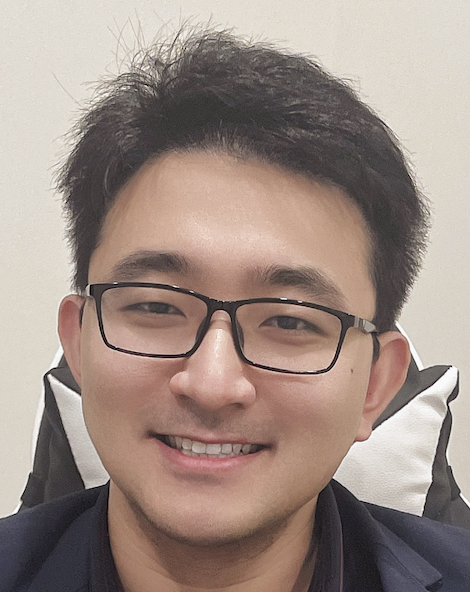
\includegraphics[width=1in,height=1.25in,clip,keepaspectratio]{images/Tianming_Zhao.png}}]
{Tianming Zhao} received his Ph.D. from the School of Computer Science, The University of Sydney in 2023. He is currently a postdoctoral researcher at the Center for Distributed and High Performance Computing, School of Computer Science, The University of Sydney. His research interests include algorithms with predictions, scheduling, and quantitative research. He was awarded the University Medal for his B.S. degree with Honors in computer science from The University of Sydney. He received the IEEE TCSC Outstanding Ph.D. Dissertation Award (2024). 
\end{IEEEbiography}

\vspace{-30pt}




\begin{IEEEbiography}[{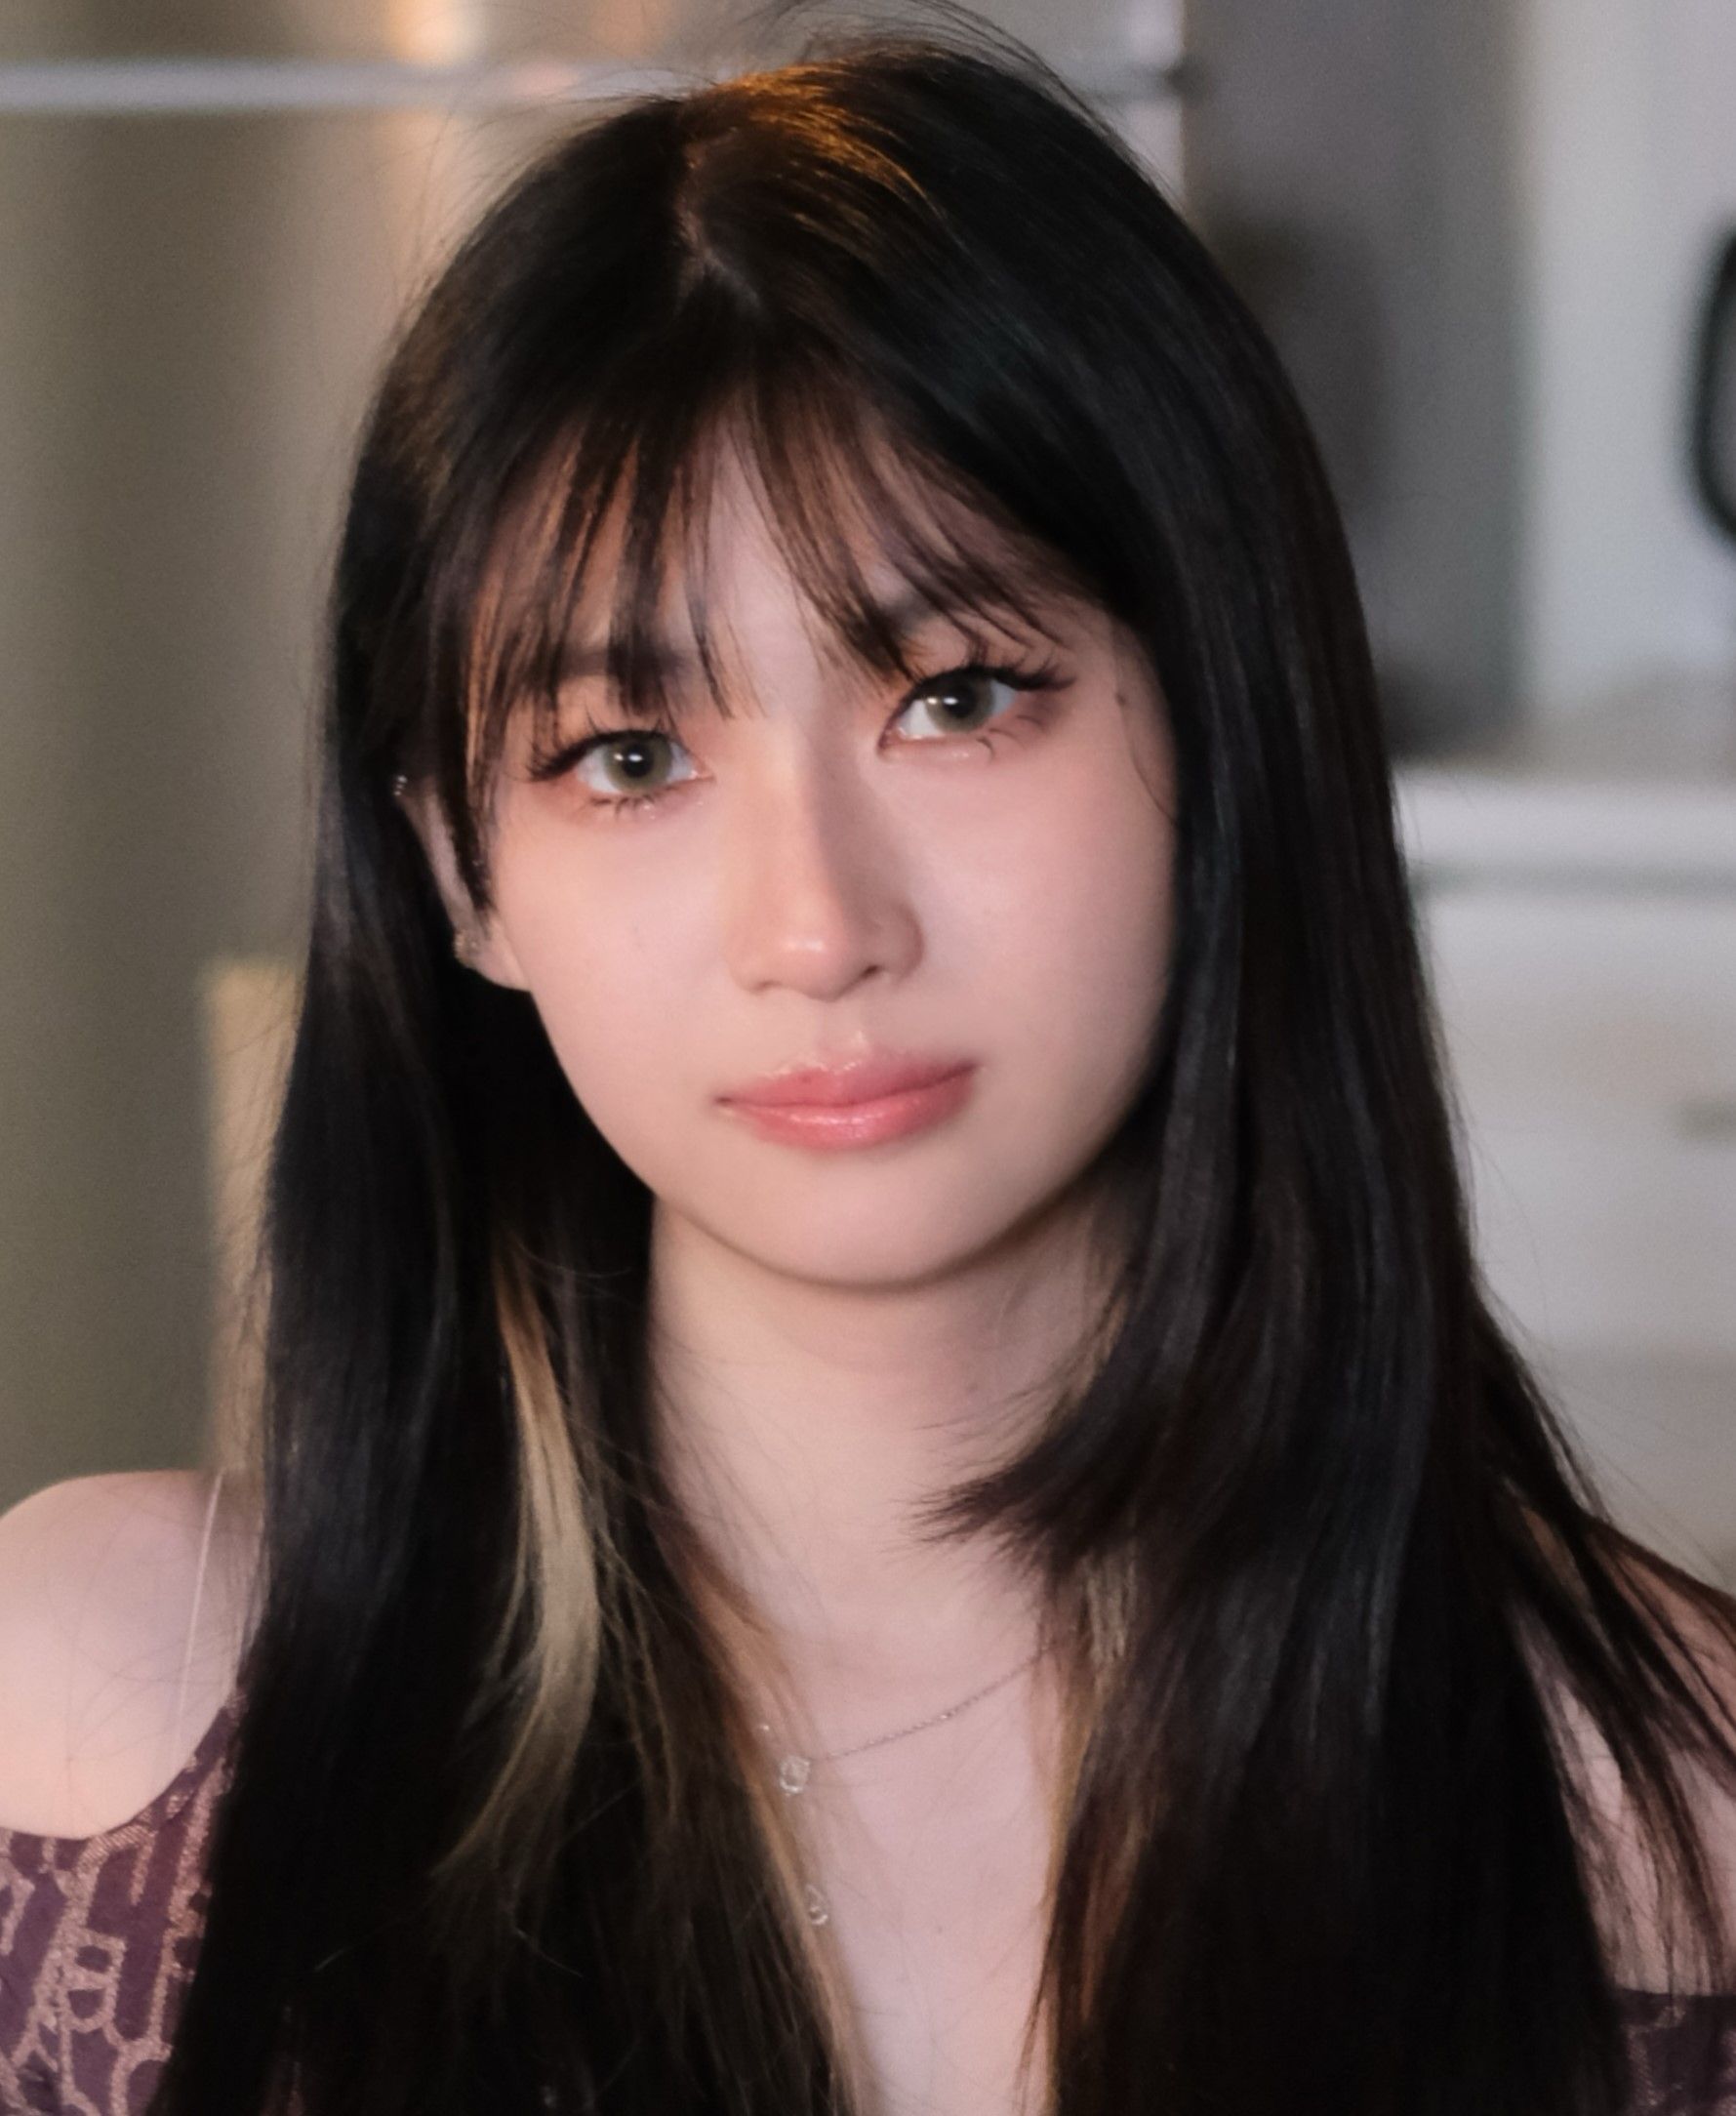
\includegraphics[width=1in,height=1.25in,clip,keepaspectratio]{images/Zhiyun1.jpg}}]
{Zhiyun Jiang} received her Bachelor Degree with Honours in Civil Engineering from The University of Sydney (2022). She further received her Master Degree of Data Science from the University of Sydney (2023) and is a currently enrolled HDR student in the School of Computer Science supervised by Professor Albert Y. Zomaya. Her research interests are in scheduling with predictions, online algorithms, and meta-scheduling. 
\end{IEEEbiography}

\vspace{-30pt}

\begin{IEEEbiography}[{\includegraphics[width=1in,height=1.25in,clip,keepaspectratio]{images/Chunqiu_xia.jpg}}]
{Chunqiu Xia} received the M.Phil. degree in 2019 and the Ph.D. degree in 2024, both from the School of Computer Science, The University of Sydney, Australia. He is currently a postdoctoral researcher at the Center for Distributed and High Performance Computing, School of Computer Science, The University of Sydney. His research interests include edge computing, the energy internet, and scheduling.
\end{IEEEbiography}

\vspace{-30pt}

\begin{IEEEbiography}[{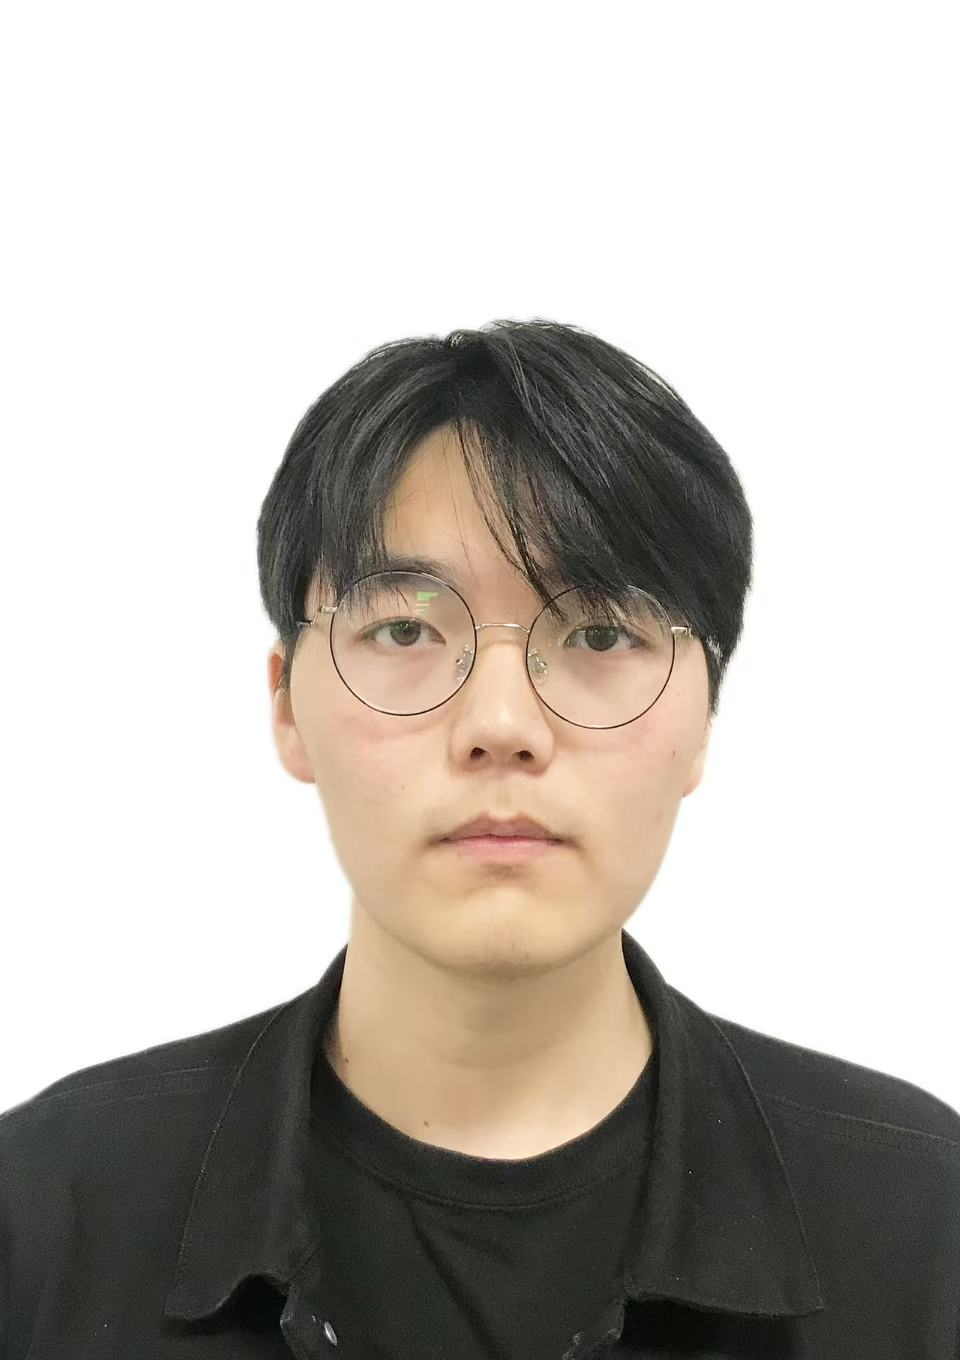
\includegraphics[width=1in,height=1.25in,clip,keepaspectratio]{images/xinweiji.jpg}}]
{Xinwei Ji} received his Ph.D. degree in 2024 from the Center for Distributed and High-Performance Computing at the University of Sydney, Australia. He is currently a postdoctoral researcher at Shenzhen University, China. His research interests include artificial intelligence in healthcare, model compression and acceleration of vision-language models, and computation resources scheduling with prediction.
\end{IEEEbiography}



\vspace{-30pt}

\begin{IEEEbiography}[{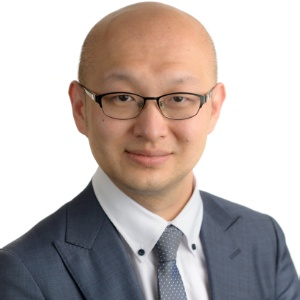
\includegraphics[width=1in,height=1.25in,clip,keepaspectratio]{images/Wei_Li.jpg}}]
{Wei Li} received his PhD degree from the School of Information Technologies at The University of Sydney. He is currently an ARC DECRA fellow at the Centre for Distributed and High-Performance Computing, School of Computer Science, The University of Sydney. His research interests include edge computing, sustainable computing, task scheduling, energy efficiency, and the Internet of Things. He is the recipient of five IEEE or ACM conference best paper awards. He received the IEEE TCSC Award for Excellence in Scalable Computing for Early Career Researchers (2018) and the IEEE Outstanding Leadership Award (2018). He is a senior member of the IEEE Computer Society and the IEEE, and a member of the ACM. He is currently an Associate Editor of IEEE TRANSACTIONS ON SUSTAINABLE COMPUTING.
\end{IEEEbiography}

\vspace{-20pt}

\begin{IEEEbiography}[{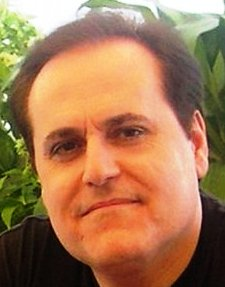
\includegraphics[width=1in,height=1.25in,clip,keepaspectratio]{images/Albert_Zomaya.jpg}}]
{Albert Y. Zomaya} is Peter Nicol Russell Chair Professor of Computer Science and Director of the Centre for Distributed and High-Performance Computing at the University of Sydney. He is the past Editor in Chief of the IEEE Transactions on Computers (2010-2014), the IEEE Transactions on Sustainable Computing (2016-2020), and the ACM Computing Surveys (2019-2024). Professor Zomaya is a decorated scholar with numerous accolades, including Fellowship of the IEEE, the American Association for the Advancement of Science, and the Institution of Engineering and Technology (UK). Also, he is an Elected Fellow of the Australian Academy of Science, the Royal Society of New South Wales, an Elected Foreign Member of Academia Europaea, and a Member of the European Academy of Science and Arts. His research interests span several areas in parallel and distributed computing and complex systems.
\end{IEEEbiography}


% that's all folks
\end{document}


